% generated by Ott 0.20.1 from: epaj_common.ott epaj_st.ott epaj_st_wf.ott epaj_rt.ott epaj_rt_wf.ott
\newcommand{\ottdrule}[4][]{{\displaystyle\frac{\begin{array}{l}#2\end{array}}{#3}\quad\ottdrulename{#4}}}
\newcommand{\ottusedrule}[1]{\[#1\]}
\newcommand{\ottpremise}[1]{ #1 \\}
\newenvironment{ottdefnblock}[3][]{ \framebox{\mbox{#2}} \quad #3 \\[0pt]}{}
\newenvironment{ottfundefnblock}[3][]{ \framebox{\mbox{#2}} \quad #3 \\[0pt]\begin{displaymath}\begin{array}{l}}{\end{array}\end{displaymath}}
\newcommand{\ottfunclause}[2]{ #1 \equiv #2 \\}
\newcommand{\ottnt}[1]{\mathit{#1}}
\newcommand{\ottmv}[1]{\mathit{#1}}
\newcommand{\ottkw}[1]{\mathbf{#1}}
\newcommand{\ottsym}[1]{#1}
\newcommand{\ottcom}[1]{\text{#1}}
\newcommand{\ottdrulename}[1]{\textsc{#1}}
\newcommand{\ottcomplu}[5]{\overline{#1}^{\,#2\in #3 #4 #5}}
\newcommand{\ottcompu}[3]{\overline{#1}^{\,#2<#3}}
\newcommand{\ottcomp}[2]{\overline{#1}^{\,#2}}
\newcommand{\ottgrammartabular}[1]{\begin{supertabular}{llcllllll}#1\end{supertabular}}
\newcommand{\ottmetavartabular}[1]{\begin{supertabular}{ll}#1\end{supertabular}}
\newcommand{\ottrulehead}[3]{$#1$ & & $#2$ & & & \multicolumn{2}{l}{#3}}
\newcommand{\ottprodline}[6]{& & $#1$ & $#2$ & $#3 #4$ & $#5$ & $#6$}
\newcommand{\ottinterrule}{\\[5.0mm]}
\newcommand{\ottafterlastrule}{\\}
\newcommand{\ottmetavars}{
\ottmetavartabular{
 $ \ottmv{i} ,\, \ottmv{j} ,\, \ottmv{k} ,\, \ottmv{n} $ & \multicolumn{1}{l}{\ottcom{index variables as arbitrary elements}} \\
 $ \ottmv{f} $ & \multicolumn{1}{l}{\ottcom{field identifier}} \\
 $ \mathit{mid} $ & \multicolumn{1}{l}{\ottcom{method identifier}} \\
 $ \mathit{pid} $ & \multicolumn{1}{l}{\ottcom{parameter identifier}} \\
 $ \mathit{Cid} $ & \multicolumn{1}{l}{\ottcom{derived class identifier}} \\
 $ \mathit{RAId} $ & \multicolumn{1}{l}{\ottcom{raw address identifier}} \\
 $ \mathit{PrimV} $ & \multicolumn{1}{l}{\ottcom{primitive value}} \\
}}

\newcommand{\ottterminals}{
\ottrulehead{\ottnt{terminals}}{::=}{}\\ 
\ottprodline{|}{ := }{}{}{}{}\\ 
\ottprodline{|}{ \texttt{\upshape{class}\,\!} }{}{}{}{\ottcom{keyword: class declaration}}\\ 
\ottprodline{|}{ \texttt{\upshape{extends}\,\!} }{}{}{}{\ottcom{keyword: super type declaration}}\\ 
\ottprodline{|}{ \texttt{\upshape{new}\,\!} }{}{}{}{\ottcom{keyword: object creation}}\\ 
\ottprodline{|}{ \texttt{\upshape{if}\,\!} }{}{}{}{\ottcom{keyword: if}}\\ 
\ottprodline{|}{ \texttt{\upshape{else}\,\!} }{}{}{}{\ottcom{keyword: else}}\\ 
\ottprodline{|}{ \texttt{\upshape{this}\,\!} }{}{}{}{\ottcom{keyword: current object}}\\ 
\ottprodline{|}{ \texttt{\upshape{null}\,\!} }{}{}{}{\ottcom{keyword: null value}}\\ 
\ottprodline{|}{ \oplus }{}{}{}{\ottcom{syntax: primitive operation}}\\ 
\ottprodline{|}{ \texttt{\{} }{}{}{}{\ottcom{syntax: start block}}\\ 
\ottprodline{|}{ \texttt{\}\,} }{}{}{}{\ottcom{syntax: end block}}\\ 
\ottprodline{|}{ \texttt{(} }{}{}{}{\ottcom{syntax: start parameters}}\\ 
\ottprodline{|}{ \texttt{)} }{}{}{}{\ottcom{syntax: end parameters}}\\ 
\ottprodline{|}{ \texttt{;} }{}{}{}{\ottcom{syntax: separator}}\\ 
\ottprodline{|}{ \texttt{.} }{}{}{}{\ottcom{syntax: selector}}\\ 
\ottprodline{|}{ \texttt{=} }{}{}{}{\ottcom{syntax: assignment}}\\ 
\ottprodline{|}{ \texttt{\upshape{Object}\,\!} }{}{}{}{\ottcom{name of root class}}\\ 
\ottprodline{|}{ \texttt{\upshape{int}\,\!} }{}{}{}{\ottcom{name of primitive type}}\\ 
\ottprodline{|}{ \mathcal{L} }{}{}{}{\ottcom{primitive literal}}\\ 
\ottprodline{|}{ \textsf{$<:_{\mathrm q}$} }{}{}{}{\ottcom{ordering of precision qualifiers}}\\ 
\ottprodline{|}{ \textsf{$<:$} }{}{}{}{\ottcom{subtyping}}\\ 
\ottprodline{|}{ \textsf{$\in$} }{}{}{}{\ottcom{containment judgement}}\\ 
\ottprodline{|}{ \textsf{$\notin$} }{}{}{}{\ottcom{non-containment judgement}}\\ 
\ottprodline{|}{ \textsf{$\vdash$} }{}{}{}{\ottcom{single element judgement}}\\ 
\ottprodline{|}{ \textsf{$\vdash$} }{}{}{}{\ottcom{multiple element judgement}}\\ 
\ottprodline{|}{ \textsf{:} }{}{}{}{\ottcom{separator}}\\ 
\ottprodline{|}{ \mapsto }{}{}{}{\ottcom{maps-to}}\\ 
\ottprodline{|}{ \textsf{OK} }{}{}{}{\ottcom{well-formedness judgement}}\\ 
\ottprodline{|}{ \textsf{=} }{}{}{}{\ottcom{alias}}\\ 
\ottprodline{|}{ \textsf{=} }{}{}{}{\ottcom{option alias}}\\ 
\ottprodline{|}{ \textsf{$\not=$} }{}{}{}{\ottcom{not alias}}\\ 
\ottprodline{|}{ \textsf{=} }{}{}{}{\ottcom{multiple alias}}\\ 
\ottprodline{|}{ \textsf{$\vee$} }{}{}{}{\ottcom{logical or}}\\ 
\ottprodline{|}{ \textsf{$\wedge$} }{}{}{}{\ottcom{logical and}}\\ 
\ottprodline{|}{\ottkw{AND}}{}{}{}{\ottcom{top-level logical and}}\\ 
\ottprodline{|}{ \textsf{$\implies$} }{}{}{}{\ottcom{logical implication}}\\ 
\ottprodline{|}{ \texttt{\upshape{null$_a$}\,\!} }{}{}{}{\ottcom{special null address}}\\ 
\ottprodline{|}{ \rho }{}{}{}{\ottcom{primitive values}}\\ 
\ottprodline{|}{ 0 }{}{}{}{\ottcom{zero value}}}

\newcommand{\ottformula}{
\ottrulehead{\ottnt{formula}}{::=}{\ottcom{formulas}}\\ 
\ottprodline{|}{ \mathrm{otherwise} }{}{}{}{\ottcom{none of the previous rules applied}}\\ 
\ottprodline{|}{\ottnt{judgement}}{}{}{}{\ottcom{judgement}}\\ 
\ottprodline{|}{\ottnt{formula_{{\mathrm{1}}}} \quad \ottsym{,} \quad .. \quad \ottsym{,} \quad \ottnt{formula_{\ottmv{k}}}}{}{}{}{\ottcom{sequence}}\\ 
\ottprodline{|}{ ( \ottnt{formula} ) }{}{}{}{\ottcom{bracketed}}\\ 
\ottprodline{|}{ !  \ottnt{formula} }{}{}{}{\ottcom{negation}}\\ 
\ottprodline{|}{ \ottnt{formula} \ \  \textsf{$\vee$} \ \  \ottnt{formula'} }{}{}{}{\ottcom{logical or}}\\ 
\ottprodline{|}{ \ottnt{formula} \ \  \textsf{$\wedge$} \ \  \ottnt{formula'} }{}{}{}{\ottcom{logical and}}\\ 
\ottprodline{|}{ \hfill  \ottnt{formula}  \hfill\hspace{7mm plus 2mm minus 1mm}\hfill  \ottnt{formula'} \hfill }{}{}{}{\ottcom{top-level logical and}}\\ 
\ottprodline{|}{\ottnt{formula}  \textsf{$\implies$}  \ottnt{formula'}}{}{}{}{\ottcom{implies}}\\ 
\ottprodline{|}{\overline{^{s}\!fml}}{}{}{}{\ottcom{static formulas}}\\ 
\ottprodline{|}{\overline{^{r}\!fml}}{}{}{}{\ottcom{runtime formulas}}\\ 
\ottprodline{|}{ \forall  \ottmv{f}  \in  \overline{f} .\  \ottnt{formula} }{}{}{}{\ottcom{for all $\ottmv{f}$ in $\overline{f}$ holds $\ottnt{formula}$}}\\ 
\ottprodline{|}{ \forall  \ottnt{C} ,  \ottnt{C'} .\  \ottnt{formula} }{}{}{}{\ottcom{for all $\ottnt{C}$ and $\ottnt{C'}$ holds $\ottnt{formula}$}}\\ 
\ottprodline{|}{ \forall  \iota  \in  \overline{\iota} .\  \ottnt{formula} }{}{}{}{\ottcom{for all $\iota$ in $\overline{\iota}$ holds $\ottnt{formula}$}}\\ 
\ottprodline{|}{ \forall  \iota  \in  \overline{\iota} ,  \ottmv{f}  \in  \overline{\mathit{fv} } .\  \ottnt{formula} }{}{}{}{\ottcom{for all $\iota$ in $\overline{\iota}$ and fields $\ottmv{f}$ in $\overline{\mathit{fv} }$ holds $\ottnt{formula}$}}\\ 
\ottprodline{|}{ \ottnt{h}  \cong  \ottnt{h'} }{}{}{}{\ottcom{two heaps are equal in their precise part}}\\ 
\ottprodline{|}{ v  \cong  v' }{}{}{}{\ottcom{two values are equal in their precise parts}}}

\newcommand{\ottC}{
\ottrulehead{\ottnt{C}}{::=}{\ottcom{class name}}\\ 
\ottprodline{|}{\mathit{Cid}}{}{}{}{\ottcom{derived class identifier}}\\ 
\ottprodline{|}{\texttt{\upshape{Object}\,\!}}{}{}{}{\ottcom{name of base class}}\\ 
\ottprodline{|}{ \texttt{\_} } {\textsf{M}}{}{}{\ottcom{some class name}}}

\newcommand{\ottP}{
\ottrulehead{\ottnt{P}}{::=}{\ottcom{primitive type name}}\\ 
\ottprodline{|}{\texttt{\upshape{int}\,\!}}{}{}{}{\ottcom{integers}}\\ 
\ottprodline{|}{\ottkw{float}}{}{}{}{\ottcom{floating-point numbers}}}

\newcommand{\ottq}{
\ottrulehead{\ottnt{q}}{::=}{\ottcom{precision qualifier}}\\ 
\ottprodline{|}{ \texttt{\upshape{precise}\,\!} }{}{}{}{\ottcom{precise}}\\ 
\ottprodline{|}{ \texttt{\upshape{approx}\,\!} }{}{}{}{\ottcom{approximate}}\\ 
\ottprodline{|}{ \texttt{\upshape{top}\,\!} }{}{}{}{\ottcom{top}}\\ 
\ottprodline{|}{ \texttt{\upshape{context}\,\!} }{}{}{}{\ottcom{context}}\\ 
\ottprodline{|}{ \texttt{\upshape{lost}\,\!} }{}{}{}{\ottcom{lost}}\\ 
\ottprodline{|}{ \mathrm{TQual}\!\left(  T  \right) } {\textsf{M}}{}{}{\ottcom{extract precision qualifier from type}}\\ 
\ottprodline{|}{ \mathrm{MQual}\!\left(  \ottnt{ms}  \right) } {\textsf{M}}{}{}{\ottcom{extract method qualifier from signature}}\\ 
\ottprodline{|}{ \mathit{ {^r}\!\Gamma} \!\!\downarrow_{1} } {\textsf{M}}{}{}{\ottcom{extract environment qualifier}}}

\newcommand{\ottqs}{
\ottrulehead{\overline{q}}{::=}{\ottcom{precision qualfiers}}\\ 
\ottprodline{|}{\ottnt{q_{{\mathrm{1}}}}  \ottsym{,} \, .. \, \ottsym{,}  \ottnt{q_{\ottmv{n}}}}{}{}{}{\ottcom{precision qualifier list}}\\ 
\ottprodline{|}{ \left\{  \overline{q}  \right\} } {\textsf{M}}{}{}{\ottcom{notation}}}

\newcommand{\ottqC}{
\ottrulehead{\ottnt{qC}}{::=}{\ottcom{qualified class name}}\\ 
\ottprodline{|}{ \ottnt{q} \  \ottnt{C} }{}{}{}{\ottcom{definition}}}

\newcommand{\ottqP}{
\ottrulehead{\ottnt{qP}}{::=}{\ottcom{qualified primitive type}}\\ 
\ottprodline{|}{ \ottnt{q} \  \ottnt{P} }{}{}{}{\ottcom{definition}}}

\newcommand{\ottT}{
\ottrulehead{T}{::=}{\ottcom{type}}\\ 
\ottprodline{|}{ \ottnt{qC} }{}{}{}{\ottcom{reference type}}\\ 
\ottprodline{|}{ \ottnt{qP} }{}{}{}{\ottcom{primitive type}}\\ 
\ottprodline{|}{ \texttt{\_} } {\textsf{M}}{}{}{\ottcom{some type}}\\ 
\ottprodline{|}{ \mathit{ {^s}\!\Gamma} \!\left( \ottnt{x} \right) } {\textsf{M}}{}{}{\ottcom{look up parameter type}}\\ 
\ottprodline{|}{ \ottnt{h} \!\left( \iota \right)\!\!\downarrow_{1} } {\textsf{M}}{}{}{\ottcom{look up type in heap}}}

\newcommand{\ottTs}{
\ottrulehead{\overline{T}}{::=}{\ottcom{types}}\\ 
\ottprodline{|}{T_{{\mathrm{1}}}  \ottsym{,} \, .. \, \ottsym{,}  T_{\ottmv{n}}}{}{}{}{\ottcom{type list}}\\ 
\ottprodline{|}{ \overline{T}_{{\mathrm{1}}} ,\  \overline{T}_{{\mathrm{2}}} }{}{}{}{\ottcom{two type lists}}\\ 
\ottprodline{|}{ \emptyset }{}{}{}{\ottcom{no types}}\\ 
\ottprodline{|}{ \texttt{\_} } {\textsf{M}}{}{}{\ottcom{some types}}}

\newcommand{\ottPrg}{
\ottrulehead{\ottnt{Prg}}{::=}{\ottcom{program}}\\ 
\ottprodline{|}{ \overline{\mathit{Cls} } ,\  \ottnt{C} ,\  \ottnt{e} }{}{}{}{}}

\newcommand{\ottCls}{
\ottrulehead{\mathit{Cls}}{::=}{\ottcom{class declaration}}\\ 
\ottprodline{|}{ \texttt{\upshape{class}\,\!} \  \mathit{Cid} \  \texttt{\upshape{extends}\,\!} \  \ottnt{C} \  \texttt{\{} \  \overline{ \mathit{fd} } \  \overline{ \mathit{md} } \  \texttt{\}\,} }{}{}{}{\ottcom{class declaration}}\\ 
\ottprodline{|}{ \texttt{\upshape{class}\,\!} \  \texttt{\upshape{Object}\,\!} \  \texttt{\{} \texttt{\}\,} }{}{}{}{\ottcom{declaration of base class}}}

\newcommand{\ottClss}{
\ottrulehead{\overline{\mathit{Cls} }}{::=}{\ottcom{class declarations}}\\ 
\ottprodline{|}{\mathit{Cls}_{{\mathrm{1}}} \, .. \, \mathit{Cls}_{\ottmv{n}}}{}{}{}{\ottcom{class declaration list}}}

\newcommand{\ottfds}{
\ottrulehead{\overline{ \mathit{fd} }}{::=}{\ottcom{field declarations}}\\ 
\ottprodline{|}{ T \  \ottmv{f} \texttt{;} }{}{}{}{\ottcom{type $T$ and field name $\ottmv{f}$}}\\ 
\ottprodline{|}{\overline{ \mathit{fd} }_{{\mathrm{1}}} \, .. \, \overline{ \mathit{fd} }_{\ottmv{n}}}{}{}{}{\ottcom{field declaration list}}\\ 
\ottprodline{|}{ \texttt{\_} } {\textsf{M}}{}{}{\ottcom{some field declarations}}}

\newcommand{\ottfs}{
\ottrulehead{\overline{f}}{::=}{\ottcom{list of field identifiers}}\\ 
\ottprodline{|}{\ottmv{f_{{\mathrm{1}}}} \, .. \, \ottmv{f_{\ottmv{n}}}}{}{}{}{\ottcom{field identifier list}}\\ 
\ottprodline{|}{ \mathrm{refFields}\!\left( \ottnt{C} \right) } {\textsf{M}}{}{}{\ottcom{recursive reference type fields look-up}}\\ 
\ottprodline{|}{ \mathrm{primFields}\!\left( \ottnt{C} \right) } {\textsf{M}}{}{}{\ottcom{recursive primitive type fields look-up}}}

\newcommand{\otte}{
\ottrulehead{\ottnt{e}}{::=}{\ottcom{expression}}\\ 
\ottprodline{|}{\texttt{\upshape{null}\,\!}}{}{}{}{\ottcom{null expression}}\\ 
\ottprodline{|}{\mathcal{L}}{}{}{}{\ottcom{primitive literal}}\\ 
\ottprodline{|}{\ottnt{x}}{}{}{}{\ottcom{variable read}}\\ 
\ottprodline{|}{ \texttt{\upshape{new}\,\!} \  \ottnt{qC} \texttt{(} \texttt{)} }{}{}{}{\ottcom{object construction}}\\ 
\ottprodline{|}{ \ottnt{e} \texttt{.} \ottmv{f} }{}{}{}{\ottcom{field read}}\\ 
\ottprodline{|}{ \ottnt{e_{{\mathrm{0}}}} \texttt{.} \ottmv{f} \  := \  \ottnt{e_{{\mathrm{1}}}} }{}{}{}{\ottcom{field write}}\\ 
\ottprodline{|}{\ottnt{e_{{\mathrm{0}}}}  \texttt{.}  \ottnt{m}  \texttt{(}  \overline{e}  \texttt{)}}{}{}{}{\ottcom{method call}}\\ 
\ottprodline{|}{ \texttt{(} \ottnt{qC} \texttt{)} \  \ottnt{e} }{}{}{}{\ottcom{cast}}\\ 
\ottprodline{|}{\ottnt{e_{{\mathrm{0}}}}  \oplus  \ottnt{e_{{\mathrm{1}}}}}{}{}{}{\ottcom{primitive operation}}\\ 
\ottprodline{|}{ \texttt{\upshape{if}\,\!} ( \ottnt{e_{{\mathrm{0}}}} )\  \texttt{\{}   \ottnt{e_{{\mathrm{1}}}}   \texttt{\}\,} \  \texttt{\upshape{else}\,\!} \  \texttt{\{}   \ottnt{e_{{\mathrm{2}}}}   \texttt{\}\,} }{}{}{}{\ottcom{conditional}}\\ 
\ottprodline{|}{ \textit{None} } {\textsf{M}}{}{}{\ottcom{no expression defined}}}

\newcommand{\ottes}{
\ottrulehead{\overline{e}}{::=}{\ottcom{expressions}}\\ 
\ottprodline{|}{\ottnt{e_{{\mathrm{1}}}}  \ottsym{,} \, .. \, \ottsym{,}  \ottnt{e_{\ottmv{k}}}}{}{}{}{\ottcom{list of expressions}}\\ 
\ottprodline{|}{ \emptyset }{}{}{}{\ottcom{empty list}}}

\newcommand{\ottmd}{
\ottrulehead{\mathit{md}}{::=}{\ottcom{method declaration}}\\ 
\ottprodline{|}{ \ottnt{ms}  \  \texttt{\{} \  \ottnt{e} \  \texttt{\}\,} }{}{}{}{\ottcom{method signature and method body}}}

\newcommand{\ottmds}{
\ottrulehead{\overline{ \mathit{md} }}{::=}{\ottcom{method declarations}}\\ 
\ottprodline{|}{\mathit{md}}{}{}{}{\ottcom{method declaration}}\\ 
\ottprodline{|}{\overline{ \mathit{md} }_{{\mathrm{1}}} \, .. \, \overline{ \mathit{md} }_{\ottmv{n}}}{}{}{}{\ottcom{method declaration list}}\\ 
\ottprodline{|}{ \texttt{\_} } {\textsf{M}}{}{}{\ottcom{some method declarations}}}

\newcommand{\ottms}{
\ottrulehead{\ottnt{ms}}{::=}{\ottcom{method signature}}\\ 
\ottprodline{|}{ T \  \ottnt{m} \texttt{(}   \overline{\mathit{mpd} }   \texttt{)} \  \ottnt{q} }{}{}{}{\ottcom{method signature definition}}\\ 
\ottprodline{|}{ \textit{None} } {\textsf{M}}{}{}{\ottcom{no method signature defined}}}

\newcommand{\ottm}{
\ottrulehead{\ottnt{m}}{::=}{\ottcom{method name}}\\ 
\ottprodline{|}{\mathit{mid}}{}{}{}{\ottcom{method identifier}}\\ 
\ottprodline{|}{ \mathrm{MName}\!\left(  \ottnt{ms}  \right) } {\textsf{M}}{}{}{\ottcom{extract method name from signature}}}

\newcommand{\ottmpds}{
\ottrulehead{\overline{\mathit{mpd} }}{::=}{\ottcom{method parameter declarations}}\\ 
\ottprodline{|}{ T \  \mathit{pid} }{}{}{}{\ottcom{type and parameter name}}\\ 
\ottprodline{|}{\overline{\mathit{mpd} }_{{\mathrm{1}}}  \ottsym{,} \, .. \, \ottsym{,}  \overline{\mathit{mpd} }_{\ottmv{n}}}{}{}{}{\ottcom{list}}\\ 
\ottprodline{|}{ \texttt{\_} } {\textsf{M}}{}{}{\ottcom{some method parameter declarations}}}

\newcommand{\ottx}{
\ottrulehead{\ottnt{x}}{::=}{\ottcom{parameter name}}\\ 
\ottprodline{|}{\mathit{pid}}{}{}{}{\ottcom{parameter identifier}}\\ 
\ottprodline{|}{\texttt{\upshape{this}\,\!}}{}{}{}{\ottcom{name of current object}}}

\newcommand{\ottsG}{
\ottrulehead{\mathit{ {^s}\!\Gamma}}{::=}{\ottcom{static environment}}\\ 
\ottprodline{|}{ \left\{  {^s}\delta  \right\} }{}{}{}{\ottcom{composition}}}

\newcommand{\ottsVEP}{
\ottrulehead{{^{s}\delta_{p} }}{::=}{\ottcom{static variable parameter environment}}\\ 
\ottprodline{|}{ \mathit{pid}   \mapsto   T }{}{}{}{\ottcom{variable $\mathit{pid}$ has type $T$}}}

\newcommand{\ottsVET}{
\ottrulehead{{^{s}\delta_{t} }}{::=}{\ottcom{static variable environment for \texttt{\upshape{this}\,\!}}}\\ 
\ottprodline{|}{ \texttt{\upshape{this}\,\!}   \mapsto   T }{}{}{}{\ottcom{variable \texttt{\upshape{this}\,\!} has type $T$}}}

\newcommand{\ottsVE}{
\ottrulehead{{^s}\delta}{::=}{\ottcom{static variable environment}}\\ 
\ottprodline{|}{{^{s}\delta_{t} }}{}{}{}{\ottcom{mapping for \texttt{\upshape{this}\,\!}}}\\ 
\ottprodline{|}{ {^{s}\delta_{t} } , \texttt{\_} }{}{}{}{\ottcom{mapping for \texttt{\upshape{this}\,\!} and some others}}\\ 
\ottprodline{|}{{^{s}\delta_{t} }  \ottsym{,}  {^{s}\delta_{p} }_{{\mathrm{1}}}  \ottsym{,} \, .. \, \ottsym{,}  {^{s}\delta_{p} }_{\ottmv{i}}}{}{}{}{\ottcom{mappings list}}}

\newcommand{\ottstXXfmls}{
\ottrulehead{\overline{^{s}\!fml}}{::=}{\ottcom{static formulas}}\\ 
\ottprodline{|}{\ottnt{Prg}  \textsf{=}  \ottnt{Prg'}}{}{}{}{\ottcom{program alias}}\\ 
\ottprodline{|}{\ottnt{C}  \textsf{=}  \ottnt{C'}}{}{}{}{\ottcom{class alias}}\\ 
\ottprodline{|}{T  \textsf{=}  T'}{}{}{}{\ottcom{type alias}}\\ 
\ottprodline{|}{T  \textsf{=}  T'}{}{}{}{\ottcom{option type alias}}\\ 
\ottprodline{|}{\ottnt{q}  \textsf{=}  \ottnt{q'}}{}{}{}{\ottcom{qualifier alias}}\\ 
\ottprodline{|}{\ottnt{q}  \textsf{$\not=$}  \ottnt{q'}}{}{}{}{\ottcom{qualifier not alias}}\\ 
\ottprodline{|}{\ottnt{q} \, \textsf{$\in$} \, \overline{q}}{}{}{}{\ottcom{qualifier in set of qualifiers}}\\ 
\ottprodline{|}{\ottnt{q} \, \textsf{$\notin$} \, \overline{T}}{}{}{}{\ottcom{qualifier in set of types}}\\ 
\ottprodline{|}{\ottnt{m}  \textsf{=}  \ottnt{m'}}{}{}{}{\ottcom{method name alias}}\\ 
\ottprodline{|}{\ottnt{m}  \textsf{$\not=$}  \ottnt{m'}}{}{}{}{\ottcom{method name not alias}}\\ 
\ottprodline{|}{\ottnt{ms}  \textsf{=}  \ottnt{ms'}}{}{}{}{\ottcom{method signature alias}}\\ 
\ottprodline{|}{\mathit{ {^s}\!\Gamma}  \textsf{=}  \mathit{ {^s}\!\Gamma}'}{}{}{}{\ottcom{static environment alias}}\\ 
\ottprodline{|}{\ottnt{e}  \textsf{=}  \ottnt{e'}}{}{}{}{\ottcom{expression alias}}\\ 
\ottprodline{|}{\mathit{Cls} \, \textsf{$\in$} \, \ottnt{Prg}}{}{}{}{\ottcom{class definition in program}}\\ 
\ottprodline{|}{ \texttt{\upshape{class}\,\!} \  \ottnt{C}  \ldots \in  \ottnt{Prg} }{}{}{}{\ottcom{partial class definition in program}}}

\newcommand{\ottii}{
\ottrulehead{\iota}{::=}{\ottcom{address identifier}}\\ 
\ottprodline{|}{\mathit{RAId}}{}{}{}{\ottcom{raw address identifier}}\\ 
\ottprodline{|}{ \mathit{ {^r}\!\Gamma} \!\left( \texttt{\upshape{this}\,\!} \right) } {\textsf{M}}{}{}{\ottcom{currently active object look-up}}\\ 
\ottprodline{|}{ \texttt{\_} } {\textsf{M}}{}{}{\ottcom{some address identifier}}}

\newcommand{\ottpp}{
\ottrulehead{{^r}\!\mathcal{L}}{::=}{\ottcom{primitive value}}\\ 
\ottprodline{|}{0}{}{}{}{\ottcom{zero value}}\\ 
\ottprodline{|}{\mathit{PrimV}}{}{}{}{\ottcom{primitive value}}\\ 
\ottprodline{|}{{^r}\!\mathcal{L}_{{\mathrm{0}}}  \oplus  {^r}\!\mathcal{L}_{{\mathrm{1}}}} {\textsf{M}}{}{}{\ottcom{binary operation}}}

\newcommand{\ottqpp}{
\ottrulehead{\rho_{q}}{::=}{\ottcom{qualified primitive value}}\\ 
\ottprodline{|}{ ( \ottnt{q} ,  {^r}\!\mathcal{L} ) }{}{}{}{\ottcom{qualified primitive value}}}

\newcommand{\ottiis}{
\ottrulehead{\overline{\iota}}{::=}{\ottcom{address identifiers}}\\ 
\ottprodline{|}{\iota_{{\mathrm{1}}}  \ottsym{,} \, .. \, \ottsym{,}  \iota_{\ottmv{n}}}{}{}{}{\ottcom{address identifier list}}\\ 
\ottprodline{|}{ \emptyset }{}{}{}{\ottcom{empty list}}\\ 
\ottprodline{|}{ \texttt{\_} } {\textsf{M}}{}{}{\ottcom{some address identifier list}}\\ 
\ottprodline{|}{ \mathrm{dom}\!\left(  \ottnt{h}  \right) } {\textsf{M}}{}{}{\ottcom{domain of heap}}}

\newcommand{\ottv}{
\ottrulehead{v}{::=}{\ottcom{value}}\\ 
\ottprodline{|}{\iota}{}{}{}{\ottcom{address identifier}}\\ 
\ottprodline{|}{\texttt{\upshape{null$_a$}\,\!}}{}{}{}{\ottcom{null value}}\\ 
\ottprodline{|}{\rho_{q}}{}{}{}{\ottcom{qualified primitive value}}\\ 
\ottprodline{|}{ \texttt{\_} } {\textsf{M}}{}{}{\ottcom{some value}}\\ 
\ottprodline{|}{ \tilde{ v } }{}{}{}{\ottcom{similarity}}\\ 
\ottprodline{|}{ \ottnt{h} \!\left( \iota \texttt{.} \ottmv{f} \right) } {\textsf{M}}{}{}{\ottcom{field value look-up}}\\ 
\ottprodline{|}{ \mathit{ {^r}\!\Gamma} \!\left( \ottnt{x} \right) } {\textsf{M}}{}{}{\ottcom{argument value look-up}}\\ 
\ottprodline{|}{ \overline{\mathit{fv} } \!\left(  \ottmv{f}  \right) } {\textsf{M}}{}{}{\ottcom{field value look-up}}}

\newcommand{\ottvs}{
\ottrulehead{\overline{v}}{::=}{\ottcom{values}}\\ 
\ottprodline{|}{v_{{\mathrm{1}}}  \ottsym{,} \, .. \, \ottsym{,}  v_{\ottmv{n}}}{}{}{}{\ottcom{value list}}\\ 
\ottprodline{|}{ \emptyset }{}{}{}{\ottcom{empty list}}}

\newcommand{\ottfvs}{
\ottrulehead{\overline{\mathit{fv} }}{::=}{\ottcom{field values}}\\ 
\ottprodline{|}{\ottmv{f}  \mapsto  v}{}{}{}{\ottcom{field $\ottmv{f}$ has value $v$}}\\ 
\ottprodline{|}{\overline{\mathit{fv} }_{{\mathrm{1}}}  \ottsym{,} \, .. \, \ottsym{,}  \overline{\mathit{fv} }_{\ottmv{n}}}{}{}{}{\ottcom{field value list}}\\ 
\ottprodline{|}{ \_ } {\textsf{M}}{}{}{\ottcom{some field values}}\\ 
\ottprodline{|}{ \ottnt{h} \!\left( \iota \right)\!\!\downarrow_{2} } {\textsf{M}}{}{}{\ottcom{look up field values in heap}}\\ 
\ottprodline{|}{ \overline{\mathit{fv} } \!\left[  \ottmv{f}   \mapsto   v  \right] } {\textsf{M}}{}{}{\ottcom{update existing field $\ottmv{f}$ to $v$}}}

\newcommand{\otto}{
\ottrulehead{\ottnt{o}}{::=}{\ottcom{object}}\\ 
\ottprodline{|}{ \left( T ,  \overline{\mathit{fv} } \right) }{}{}{}{\ottcom{type $T$ and field values $\overline{\mathit{fv} }$}}\\ 
\ottprodline{|}{ \ottnt{h} \!\left(  \iota  \right) } {\textsf{M}}{}{}{\ottcom{look up object in heap}}}

\newcommand{\otthe}{
\ottrulehead{\mathit{he}}{::=}{\ottcom{heap entry}}\\ 
\ottprodline{|}{ \left( \iota   \mapsto   \ottnt{o} \right) }{}{}{}{\ottcom{address $\iota$ maps to object $\ottnt{o}$}}}

\newcommand{\otth}{
\ottrulehead{\ottnt{h}}{::=}{\ottcom{heap}}\\ 
\ottprodline{|}{ \emptyset }{}{}{}{\ottcom{empty heap}}\\ 
\ottprodline{|}{\ottnt{h}  \oplus  \mathit{he}}{}{}{}{\ottcom{add $\mathit{he}$ to $\ottnt{h}$, overwriting existing mappings}}\\ 
\ottprodline{|}{ \tilde{ \ottnt{h} } }{}{}{}{\ottcom{similarity}}}

\newcommand{\ottrG}{
\ottrulehead{\mathit{ {^r}\!\Gamma}}{::=}{\ottcom{runtime environment}}\\ 
\ottprodline{|}{ \left\{  \ottnt{q} ;  {^{r}\delta}  \right\} }{}{}{}{\ottcom{composition}}\\ 
\ottprodline{|}{\mathit{ {^r}\!\Gamma}  \texttt{(}  \ottnt{q}  \texttt{)}} {\textsf{M}}{}{}{\ottcom{update the precision in environment $\mathit{ {^r}\!\Gamma}$}}}

\newcommand{\ottrVEP}{
\ottrulehead{{^{r}\delta_{p} }}{::=}{\ottcom{runtime variable environment parameter entry}}\\ 
\ottprodline{|}{ \mathit{pid}   \mapsto   v }{}{}{}{\ottcom{variable $\mathit{pid}$ has value $v$}}}

\newcommand{\ottrVET}{
\ottrulehead{{^{r}\delta_{t} }}{::=}{\ottcom{runtime variable environment entry for \texttt{\upshape{this}\,\!}}}\\ 
\ottprodline{|}{ \texttt{\upshape{this}\,\!}   \mapsto   \iota }{}{}{}{\ottcom{variable \texttt{\upshape{this}\,\!} has address $\iota$}}}

\newcommand{\ottrVE}{
\ottrulehead{{^{r}\delta}}{::=}{\ottcom{runtime variable environment}}\\ 
\ottprodline{|}{{^{r}\delta_{t} }}{}{}{}{\ottcom{mapping for \texttt{\upshape{this}\,\!}}}\\ 
\ottprodline{|}{ {^{r}\delta_{t} } , \texttt{\_} }{}{}{}{\ottcom{mapping for \texttt{\upshape{this}\,\!} and some others}}\\ 
\ottprodline{|}{{^{r}\delta_{t} }  \ottsym{,}  {^{r}\delta_{p} }_{{\mathrm{1}}}  \ottsym{,} \, .. \, \ottsym{,}  {^{r}\delta_{p} }_{\ottmv{k}}}{}{}{}{\ottcom{mappings list}}}

\newcommand{\ottrtXXfmls}{
\ottrulehead{\overline{^{r}\!fml}}{::=}{\ottcom{runtime formulas}}\\ 
\ottprodline{|}{\ottnt{h}  \textsf{=}  \ottnt{h'}}{}{}{}{\ottcom{heap alias}}\\ 
\ottprodline{|}{{^r}\!\mathcal{L}  \textsf{=}  {^r}\!\mathcal{L}'}{}{}{}{\ottcom{primitive value alias}}\\ 
\ottprodline{|}{{^r}\!\mathcal{L}  \textsf{$\not=$}  {^r}\!\mathcal{L}'}{}{}{}{\ottcom{primitive value not alias}}\\ 
\ottprodline{|}{{^r}\!\mathcal{L} \, \textsf{$\in$} \, \ottnt{P}}{}{}{}{\ottcom{primitive value has primitive type}}\\ 
\ottprodline{|}{v  \textsf{=}  v'}{}{}{}{\ottcom{value alias}}\\ 
\ottprodline{|}{v  \textsf{$\not=$}  v'}{}{}{}{\ottcom{value not alias}}\\ 
\ottprodline{|}{v  \textsf{=}  v'}{}{}{}{\ottcom{value alias}}\\ 
\ottprodline{|}{\ottnt{o}  \textsf{=}  \ottnt{o'}}{}{}{}{\ottcom{object alias}}\\ 
\ottprodline{|}{\iota \, \textsf{$\in$} \, \overline{\iota}}{}{}{}{\ottcom{address in addresses}}\\ 
\ottprodline{|}{\overline{\iota}  \textsf{$\not=$}  \overline{\iota}'}{}{}{}{\ottcom{addresses not aliased}}\\ 
\ottprodline{|}{\iota \, \textsf{$\notin$} \, \overline{\iota}}{}{}{}{\ottcom{address not in addresses}}\\ 
\ottprodline{|}{ \ottmv{f}  \in \mathrm{dom}\!\left(  \overline{\mathit{fv} }  \right) }{}{}{}{\ottcom{field identifier $\ottmv{f}$ contained in domain of $\overline{\mathit{fv} }$}}\\ 
\ottprodline{|}{\ottnt{x} \, \textsf{$\in$} \, \mathit{ {^r}\!\Gamma}}{}{}{}{\ottcom{parameter in runtime environment}}\\ 
\ottprodline{|}{\mathit{ {^r}\!\Gamma}  \textsf{=}  \mathit{ {^r}\!\Gamma}'}{}{}{}{\ottcom{runtime environment alias}}\\ 
\ottprodline{|}{\overline{\mathit{fv} }  \textsf{=}  \overline{\mathit{fv} }'}{}{}{}{\ottcom{fields alias}}}

\newcommand{\ottstsubxing}{
\ottrulehead{\ottnt{stsubxing}}{::=}{}\\ 
\ottprodline{|}{ \ottnt{q} \  \textsf{$<:_{\mathrm q}$} \  \ottnt{q'} }{}{}{}{\ottcom{ordering of precision qualifiers}}\\ 
\ottprodline{|}{ \ottnt{C} \ \textsf{$\sqsubseteq$}\  \ottnt{C'} }{}{}{}{\ottcom{subclassing}}\\ 
\ottprodline{|}{ T \  \textsf{$<:$} \ \  T' }{}{}{}{\ottcom{subtyping}}\\ 
\ottprodline{|}{ \overline{T} \  \textsf{$<:$} \ \  \overline{T}' }{}{}{}{\ottcom{subtypings}}\\ 
\ottprodline{|}{ \ottnt{ms} \  \textsf{$<:$} \ \  \ottnt{ms'} }{}{}{}{\ottcom{invocations of method $\ottnt{ms}$ can safely be replaced by calls to $\ottnt{ms'}$}}}

\newcommand{\ottqcombdef}{
\ottrulehead{\ottnt{qcombdef}}{::=}{}\\ 
\ottprodline{|}{ \ottnt{q} \, \rhd\,  \ottnt{q'} \ \  \textsf{=} \ \  \ottnt{q''} }{}{}{}{\ottcom{combining two precision qualifiers}}\\ 
\ottprodline{|}{ \ottnt{q} \, \rhd\,  T \ \  \textsf{=} \ \  T' }{}{}{}{\ottcom{precision qualifier - type combination}}\\ 
\ottprodline{|}{ \ottnt{q} \, \rhd\,  \overline{T} \ \  \textsf{=} \ \  \overline{T}' }{}{}{}{\ottcom{precision qualifier - types combination}}\\ 
\ottprodline{|}{ \ottnt{q} \, \rhd\,  \ottnt{ms} \ \  \textsf{=} \ \  \ottnt{ms'} }{}{}{}{\ottcom{precision qualifier - method signature combination}}}

\newcommand{\ottstXXhelpers}{
\ottrulehead{\ottnt{st\_helpers}}{::=}{}\\ 
\ottprodline{|}{ \mathrm{FType}\!\left( \ottnt{C} ,  \ottmv{f} \right)\  \textsf{=} \  T }{}{}{}{\ottcom{look up field $\ottmv{f}$ in class $\ottnt{C}$}}\\ 
\ottprodline{|}{ \mathrm{FType}\!\left( \ottnt{qC} ,  \ottmv{f} \right)\  \textsf{=} \  T }{}{}{}{\ottcom{look up field $\ottmv{f}$ in reference type $\ottnt{qC}$}}\\ 
\ottprodline{|}{ \mathrm{MSig}\!\left( \ottnt{C} ,  \ottnt{m} ,  \ottnt{q} \right)\  \textsf{=} \  \ottnt{ms} }{}{}{}{\ottcom{look up signature of method $\ottnt{m}$ in class $\ottnt{C}$}}\\ 
\ottprodline{|}{ \mathrm{MSig}\!\left( \ottnt{qC} ,  \ottnt{m} \right)\  \textsf{=} \  \ottnt{ms} }{}{}{}{\ottcom{look up signature of method $\ottnt{m}$ in reference type $\ottnt{qC}$}}}

\newcommand{\otttyperules}{
\ottrulehead{\ottnt{typerules}}{::=}{}\\ 
\ottprodline{|}{ \mathit{ {^s}\!\Gamma} \  \textsf{$\vdash$} \  \ottnt{e} \  \textsf{:} \  T }{}{}{}{\ottcom{expression typing}}\\ 
\ottprodline{|}{ \mathit{ {^s}\!\Gamma} \  \textsf{$\vdash$} \  \overline{e} \  \textsf{:} \  \overline{T} }{}{}{}{\ottcom{expression typings}}}

\newcommand{\ottwfstatic}{
\ottrulehead{\ottnt{wfstatic}}{::=}{}\\ 
\ottprodline{|}{ T \ \  \textsf{OK} }{}{}{}{\ottcom{well-formed type}}\\ 
\ottprodline{|}{ \overline{T} \ \  \textsf{OK} }{}{}{}{\ottcom{well-formed types}}\\ 
\ottprodline{|}{ \mathit{Cls} \ \  \textsf{OK} }{}{}{}{\ottcom{well-formed class declaration}}\\ 
\ottprodline{|}{ \mathit{ {^s}\!\Gamma} \  \textsf{$\vdash$} \  T \  \ottmv{f} \texttt{;} \ \  \textsf{OK} }{}{}{}{\ottcom{well-formed field declaration}}\\ 
\ottprodline{|}{ \mathit{ {^s}\!\Gamma} \  \textsf{$\vdash$} \  \overline{ \mathit{fd} } \ \  \textsf{OK} }{}{}{}{\ottcom{well-formed field declarations}}\\ 
\ottprodline{|}{ \mathit{ {^s}\!\Gamma} ,  \ottnt{C} \  \textsf{$\vdash$} \  \mathit{md} \ \  \textsf{OK} }{}{}{}{\ottcom{well-formed method declaration}}\\ 
\ottprodline{|}{ \mathit{ {^s}\!\Gamma} ,  \ottnt{C} \  \textsf{$\vdash$} \  \overline{ \mathit{md} } \ \  \textsf{OK} }{}{}{}{\ottcom{well-formed method declarations}}\\ 
\ottprodline{|}{ \ottnt{C} \  \textsf{$\vdash$} \  \ottnt{m} \ \  \textsf{OK} }{}{}{}{\ottcom{method overriding OK}}\\ 
\ottprodline{|}{ \ottnt{C} ,  \ottnt{C'} \  \textsf{$\vdash$} \  \ottnt{m} \ \  \textsf{OK} }{}{}{}{\ottcom{method overriding OK auxiliary}}\\ 
\ottprodline{|}{ \mathit{ {^s}\!\Gamma} \ \  \textsf{OK} }{}{}{}{\ottcom{well-formed static environment}}\\ 
\ottprodline{|}{ \textsf{$\vdash$} \  \ottnt{Prg} \ \  \textsf{OK} }{}{}{}{\ottcom{well-formed program}}}

\newcommand{\ottrtXXhelpers}{
\ottrulehead{\ottnt{rt\_helpers}}{::=}{}\\ 
\ottprodline{|}{ \ottnt{h}  +  \ottnt{o} \ =\ \left( \ottnt{h'} ,  \iota \right) }{}{}{}{\ottcom{add object $\ottnt{o}$ to heap $\ottnt{h}$ resulting in heap $\ottnt{h'}$ and fresh address $\iota$}}\\ 
\ottprodline{|}{ \ottnt{h} \!\left[  \iota \texttt{.} \ottmv{f} \  := \  v  \right]\  \textsf{=} \  \ottnt{h'} }{}{}{}{\ottcom{field update in heap}}\\ 
\ottprodline{|}{ \mathrm{sTrT}\!\left( \ottnt{h} ,  \iota ,  T \right)\  \textsf{=} \  T' }{}{}{}{\ottcom{convert type $T$ to its runtime equivalent $T'$}}\\ 
\ottprodline{|}{ \ottnt{h} ,  \iota \  \textsf{$\vdash$} \  v \  \textsf{:} \ \  T }{}{}{}{\ottcom{type $T$ assignable to value $v$}}\\ 
\ottprodline{|}{ \ottnt{h} ,  \iota \  \textsf{$\vdash$} \  \overline{v} \  \textsf{:} \ \  \overline{T} }{}{}{}{\ottcom{types $\overline{T}$ assignable to values $\overline{v}$}}\\ 
\ottprodline{|}{ \mathrm{FType}\!\left( \ottnt{h} ,  \iota ,  \ottmv{f} \right)\  \textsf{=} \  T }{}{}{}{\ottcom{look up type of field in heap}}\\ 
\ottprodline{|}{ \mathrm{MSig}\!\left( \ottnt{h} ,  \iota ,  \ottnt{m} \right)\  \textsf{=} \  \ottnt{ms} }{}{}{}{\ottcom{look up method signature of method $\ottnt{m}$ at $\iota$}}\\ 
\ottprodline{|}{ \mathrm{MBody}\!\left( \ottnt{C} ,  \ottnt{m} ,  \ottnt{q} \right)\  \textsf{=} \  \ottnt{e} }{}{}{}{\ottcom{look up most-concrete body of $\ottnt{m}$, $\ottnt{q}$ in class $\ottnt{C}$ or a superclass}}\\ 
\ottprodline{|}{ \mathrm{MBody}\!\left( \ottnt{h} ,  \iota ,  \ottnt{m} \right)\  \textsf{=} \  \ottnt{e} }{}{}{}{\ottcom{look up most-concrete body of method $\ottnt{m}$ at $\iota$}}\\ 
\ottprodline{|}{ \mathrm{FVsInit}\!\left( \ottnt{qC} \right)\  \textsf{=} \  \overline{\mathit{fv} } }{}{}{}{\ottcom{initialize the fields for reference type $\ottnt{qC}$}}}

\newcommand{\ottsemantics}{
\ottrulehead{\ottnt{semantics}}{::=}{}\\ 
\ottprodline{|}{ \mathit{ {^r}\!\Gamma} \  \textsf{$\vdash$} \  \ottnt{h} ,  \ottnt{e} \ \leadsto\  \ottnt{h'} ,  v }{}{}{}{\ottcom{big-step operational semantics}}\\ 
\ottprodline{|}{ \mathit{ {^r}\!\Gamma} \  \textsf{$\vdash$} \  \ottnt{h} ,  \overline{e} \ \leadsto\  \ottnt{h'} ,  \overline{v} }{}{}{}{\ottcom{sequential big-step operational semantics}}\\ 
\ottprodline{|}{ \textsf{$\vdash$} \  \ottnt{Prg} \ \leadsto\  \ottnt{h} ,  v }{}{}{}{\ottcom{big-step operational semantics of a program}}\\ 
\ottprodline{|}{ \mathit{ {^r}\!\Gamma} \  \textsf{$\vdash$} \  \ottnt{h} ,  \ottnt{e} \ \leadsto_{c}\  \ottnt{h'} ,  v }{}{}{}{\ottcom{checked big-step operational semantics}}\\ 
\ottprodline{|}{ \mathit{ {^r}\!\Gamma} \  \textsf{$\vdash$} \  \ottnt{h} ,  \overline{e} \ \leadsto_{c}\  \ottnt{h'} ,  \overline{v} }{}{}{}{\ottcom{checked sequential big-step operational semantics}}}

\newcommand{\ottwfruntime}{
\ottrulehead{\ottnt{wfruntime}}{::=}{}\\ 
\ottprodline{|}{ \ottnt{h} \ \  \textsf{OK} }{}{}{}{\ottcom{well-formed heap}}\\ 
\ottprodline{|}{ \ottnt{h} ,  \mathit{ {^r}\!\Gamma} \  \textsf{:} \  \mathit{ {^s}\!\Gamma} \ \  \textsf{OK} }{}{}{}{\ottcom{runtime and static environments correspond}}}

\newcommand{\ottjudgement}{
\ottrulehead{\ottnt{judgement}}{::=}{}\\ 
\ottprodline{|}{\ottnt{stsubxing}}{}{}{}{}\\ 
\ottprodline{|}{\ottnt{qcombdef}}{}{}{}{}\\ 
\ottprodline{|}{\ottnt{st\_helpers}}{}{}{}{}\\ 
\ottprodline{|}{\ottnt{typerules}}{}{}{}{}\\ 
\ottprodline{|}{\ottnt{wfstatic}}{}{}{}{}\\ 
\ottprodline{|}{\ottnt{rt\_helpers}}{}{}{}{}\\ 
\ottprodline{|}{\ottnt{semantics}}{}{}{}{}\\ 
\ottprodline{|}{\ottnt{wfruntime}}{}{}{}{}}

\newcommand{\ottuserXXsyntax}{
\ottrulehead{\ottnt{user\_syntax}}{::=}{}\\ 
\ottprodline{|}{\ottmv{i}}{}{}{}{}\\ 
\ottprodline{|}{\ottmv{f}}{}{}{}{}\\ 
\ottprodline{|}{\mathit{mid}}{}{}{}{}\\ 
\ottprodline{|}{\mathit{pid}}{}{}{}{}\\ 
\ottprodline{|}{\mathit{Cid}}{}{}{}{}\\ 
\ottprodline{|}{\mathit{RAId}}{}{}{}{}\\ 
\ottprodline{|}{\mathit{PrimV}}{}{}{}{}\\ 
\ottprodline{|}{\ottnt{terminals}}{}{}{}{}\\ 
\ottprodline{|}{\ottnt{formula}}{}{}{}{}\\ 
\ottprodline{|}{\ottnt{C}}{}{}{}{}\\ 
\ottprodline{|}{\ottnt{P}}{}{}{}{}\\ 
\ottprodline{|}{\ottnt{q}}{}{}{}{}\\ 
\ottprodline{|}{\overline{q}}{}{}{}{}\\ 
\ottprodline{|}{\ottnt{qC}}{}{}{}{}\\ 
\ottprodline{|}{\ottnt{qP}}{}{}{}{}\\ 
\ottprodline{|}{T}{}{}{}{}\\ 
\ottprodline{|}{\overline{T}}{}{}{}{}\\ 
\ottprodline{|}{\ottnt{Prg}}{}{}{}{}\\ 
\ottprodline{|}{\mathit{Cls}}{}{}{}{}\\ 
\ottprodline{|}{\overline{\mathit{Cls} }}{}{}{}{}\\ 
\ottprodline{|}{\overline{ \mathit{fd} }}{}{}{}{}\\ 
\ottprodline{|}{\overline{f}}{}{}{}{}\\ 
\ottprodline{|}{\ottnt{e}}{}{}{}{}\\ 
\ottprodline{|}{\overline{e}}{}{}{}{}\\ 
\ottprodline{|}{\mathit{md}}{}{}{}{}\\ 
\ottprodline{|}{\overline{ \mathit{md} }}{}{}{}{}\\ 
\ottprodline{|}{\ottnt{ms}}{}{}{}{}\\ 
\ottprodline{|}{\ottnt{m}}{}{}{}{}\\ 
\ottprodline{|}{\overline{\mathit{mpd} }}{}{}{}{}\\ 
\ottprodline{|}{\ottnt{x}}{}{}{}{}\\ 
\ottprodline{|}{\mathit{ {^s}\!\Gamma}}{}{}{}{}\\ 
\ottprodline{|}{{^{s}\delta_{p} }}{}{}{}{}\\ 
\ottprodline{|}{{^{s}\delta_{t} }}{}{}{}{}\\ 
\ottprodline{|}{{^s}\delta}{}{}{}{}\\ 
\ottprodline{|}{\overline{^{s}\!fml}}{}{}{}{}\\ 
\ottprodline{|}{\iota}{}{}{}{}\\ 
\ottprodline{|}{{^r}\!\mathcal{L}}{}{}{}{}\\ 
\ottprodline{|}{\rho_{q}}{}{}{}{}\\ 
\ottprodline{|}{\overline{\iota}}{}{}{}{}\\ 
\ottprodline{|}{v}{}{}{}{}\\ 
\ottprodline{|}{\overline{v}}{}{}{}{}\\ 
\ottprodline{|}{\overline{\mathit{fv} }}{}{}{}{}\\ 
\ottprodline{|}{\ottnt{o}}{}{}{}{}\\ 
\ottprodline{|}{\mathit{he}}{}{}{}{}\\ 
\ottprodline{|}{\ottnt{h}}{}{}{}{}\\ 
\ottprodline{|}{\mathit{ {^r}\!\Gamma}}{}{}{}{}\\ 
\ottprodline{|}{{^{r}\delta_{p} }}{}{}{}{}\\ 
\ottprodline{|}{{^{r}\delta_{t} }}{}{}{}{}\\ 
\ottprodline{|}{{^{r}\delta}}{}{}{}{}\\ 
\ottprodline{|}{\overline{^{r}\!fml}}{}{}{}{}}

\newcommand{\ottgrammar}{\ottgrammartabular{
\ottterminals\ottinterrule
\ottformula\ottinterrule
\ottC\ottinterrule
\ottP\ottinterrule
\ottq\ottinterrule
\ottqs\ottinterrule
\ottqC\ottinterrule
\ottqP\ottinterrule
\ottT\ottinterrule
\ottTs\ottinterrule
\ottPrg\ottinterrule
\ottCls\ottinterrule
\ottClss\ottinterrule
\ottfds\ottinterrule
\ottfs\ottinterrule
\otte\ottinterrule
\ottes\ottinterrule
\ottmd\ottinterrule
\ottmds\ottinterrule
\ottms\ottinterrule
\ottm\ottinterrule
\ottmpds\ottinterrule
\ottx\ottinterrule
\ottsG\ottinterrule
\ottsVEP\ottinterrule
\ottsVET\ottinterrule
\ottsVE\ottinterrule
\ottstXXfmls\ottinterrule
\ottii\ottinterrule
\ottpp\ottinterrule
\ottqpp\ottinterrule
\ottiis\ottinterrule
\ottv\ottinterrule
\ottvs\ottinterrule
\ottfvs\ottinterrule
\otto\ottinterrule
\otthe\ottinterrule
\otth\ottinterrule
\ottrG\ottinterrule
\ottrVEP\ottinterrule
\ottrVET\ottinterrule
\ottrVE\ottinterrule
\ottrtXXfmls\ottinterrule
\ottstsubxing\ottinterrule
\ottqcombdef\ottinterrule
\ottstXXhelpers\ottinterrule
\otttyperules\ottinterrule
\ottwfstatic\ottinterrule
\ottrtXXhelpers\ottinterrule
\ottsemantics\ottinterrule
\ottwfruntime\ottinterrule

\ottafterlastrule
}}

% defnss
% defns stsubxing
% defn qorder
\newcommand{\ottdruleqqXXlost}[1]{\ottdrule[#1]{%
\ottpremise{\ottnt{q}  \textsf{$\not=$}   \texttt{\upshape{top}\,\!} }%
}{
 \ottnt{q} \  \textsf{$<:_{\mathrm q}$} \   \texttt{\upshape{lost}\,\!}  }{%
{\ottdrulename{qq\_lost}}{}%
}}


\newcommand{\ottdruleqqXXtop}[1]{\ottdrule[#1]{%
}{
 \ottnt{q} \  \textsf{$<:_{\mathrm q}$} \   \texttt{\upshape{top}\,\!}  }{%
{\ottdrulename{qq\_top}}{}%
}}


\newcommand{\ottdruleqqXXrefl}[1]{\ottdrule[#1]{%
}{
 \ottnt{q} \  \textsf{$<:_{\mathrm q}$} \  \ottnt{q} }{%
{\ottdrulename{qq\_refl}}{}%
}}

\newcommand{\ottdefnqorder}[1]{\begin{ottdefnblock}[#1]{$ \ottnt{q} \  \textsf{$<:_{\mathrm q}$} \  \ottnt{q'} $}{\ottcom{ordering of precision qualifiers}}
\ottusedrule{\ottdruleqqXXlost{}}
\ottusedrule{\ottdruleqqXXtop{}}
\ottusedrule{\ottdruleqqXXrefl{}}
\end{ottdefnblock}}


% defn subclassing
\newcommand{\ottdrulescXXdef}[1]{\ottdrule[#1]{%
\ottpremise{ \texttt{\upshape{class}\,\!} \  \mathit{Cid} \  \texttt{\upshape{extends}\,\!} \  \ottnt{C'} \  \texttt{\{} \   \texttt{\_}  \   \texttt{\_}  \  \texttt{\}\,}  \, \textsf{$\in$} \, \ottnt{Prg}}%
}{
 \mathit{Cid} \ \textsf{$\sqsubseteq$}\  \ottnt{C'} }{%
{\ottdrulename{sc\_def}}{}%
}}


\newcommand{\ottdrulescXXrefl}[1]{\ottdrule[#1]{%
\ottpremise{ \texttt{\upshape{class}\,\!} \  \ottnt{C}  \ldots \in  \ottnt{Prg} }%
}{
 \ottnt{C} \ \textsf{$\sqsubseteq$}\  \ottnt{C} }{%
{\ottdrulename{sc\_refl}}{}%
}}


\newcommand{\ottdrulescXXtrans}[1]{\ottdrule[#1]{%
\ottpremise{ \hfill   \ottnt{C} \ \textsf{$\sqsubseteq$}\  \ottnt{C_{{\mathrm{1}}}}   \hfill\hspace{7mm plus 2mm minus 1mm}\hfill   \ottnt{C_{{\mathrm{1}}}} \ \textsf{$\sqsubseteq$}\  \ottnt{C'}  \hfill }%
}{
 \ottnt{C} \ \textsf{$\sqsubseteq$}\  \ottnt{C'} }{%
{\ottdrulename{sc\_trans}}{}%
}}

\newcommand{\ottdefnsubclassing}[1]{\begin{ottdefnblock}[#1]{$ \ottnt{C} \ \textsf{$\sqsubseteq$}\  \ottnt{C'} $}{\ottcom{subclassing}}
\ottusedrule{\ottdrulescXXdef{}}
\ottusedrule{\ottdrulescXXrefl{}} \\
\ottusedrule{\ottdrulescXXtrans{}}
\end{ottdefnblock}}


% defn subtyping
\newcommand{\ottdrulestXXrefT}[1]{\ottdrule[#1]{%
\ottpremise{ \hfill   \ottnt{q} \  \textsf{$<:_{\mathrm q}$} \  \ottnt{q'}   \hfill\hspace{7mm plus 2mm minus 1mm}\hfill   \ottnt{C} \ \textsf{$\sqsubseteq$}\  \ottnt{C'}  \hfill }%
}{
   \ottnt{q} \  \ottnt{C}   \  \textsf{$<:$} \ \    \ottnt{q'} \  \ottnt{C'}   }{%
{\ottdrulename{st\_refT}}{}%
}}


\newcommand{\ottdrulestXXprimTOne}[1]{\ottdrule[#1]{%
\ottpremise{ \ottnt{q} \  \textsf{$<:_{\mathrm q}$} \  \ottnt{q'} }%
}{
   \ottnt{q} \  \ottnt{P}   \  \textsf{$<:$} \ \    \ottnt{q'} \  \ottnt{P}   }{%
{\ottdrulename{st\_primT1}}{}%
}}


\newcommand{\ottdrulestXXprimTTwo}[1]{\ottdrule[#1]{%
}{
    \texttt{\upshape{precise}\,\!}  \  \ottnt{P}   \  \textsf{$<:$} \ \     \texttt{\upshape{approx}\,\!}  \  \ottnt{P}   }{%
{\ottdrulename{st\_primT2}}{}%
}}

\newcommand{\ottdefnsubtyping}[1]{\begin{ottdefnblock}[#1]{$ T \  \textsf{$<:$} \ \  T' $}{\ottcom{subtyping}}
\ottusedrule{\ottdrulestXXrefT{}}
\ottusedrule{\ottdrulestXXprimTOne{}}
\ottusedrule{\ottdrulestXXprimTTwo{}}
\end{ottdefnblock}}


% defn subtypings
\newcommand{\ottdrulestsXXdef}[1]{\ottdrule[#1]{%
\ottpremise{\ottcomp{ T_{\ottmv{i}} \  \textsf{$<:$} \ \  T'_{\ottmv{i}} }{\ottmv{i}}}%
}{
 \ottcomp{T_{\ottmv{i}}}{\ottmv{i}} \  \textsf{$<:$} \ \  \ottcomp{T'_{\ottmv{i}}}{\ottmv{i}} }{%
{\ottdrulename{sts\_def}}{}%
}}

\newcommand{\ottdefnsubtypings}[1]{\begin{ottdefnblock}[#1]{$ \overline{T} \  \textsf{$<:$} \ \  \overline{T}' $}{\ottcom{subtypings}}
\ottusedrule{\ottdrulestsXXdef{}}
\end{ottdefnblock}}


% defn methodsubtyping
\newcommand{\ottdrulemstXXdef}[1]{\ottdrule[#1]{%
\ottpremise{ \hfill   T' \  \textsf{$<:$} \ \  T   \hfill\hspace{7mm plus 2mm minus 1mm}\hfill   \ottcomp{T_{\ottmv{k}}}{\ottmv{k}} \  \textsf{$<:$} \ \  \ottcomp{T'_{\ottmv{k}}}{\ottmv{k}}  \hfill }%
}{
  T \  \ottnt{m} \texttt{(}   \ottcomp{ T_{\ottmv{k}} \  \mathit{pid} }{\ottmv{k}}   \texttt{)} \   \texttt{\upshape{precise}\,\!}   \  \textsf{$<:$} \ \   T' \  \ottnt{m} \texttt{(}   \ottcomp{ T'_{\ottmv{k}} \  \mathit{pid} }{\ottmv{k}}   \texttt{)} \   \texttt{\upshape{approx}\,\!}   }{%
{\ottdrulename{mst\_def}}{}%
}}

\newcommand{\ottdefnmethodsubtyping}[1]{\begin{ottdefnblock}[#1]{$ \ottnt{ms} \  \textsf{$<:$} \ \  \ottnt{ms'} $}{\ottcom{invocations of method $\ottnt{ms}$ can safely be replaced by calls to $\ottnt{ms'}$}}
\ottusedrule{\ottdrulemstXXdef{}}
\end{ottdefnblock}}


\newcommand{\ottdefnsstsubxing}{
\ottdefnqorder{}
\ottdefnsubclassing{}
\ottdefnsubtyping{}
\ottdefnsubtypings{}
\ottdefnmethodsubtyping{}}


% defns qcombdef
% defn qcombqrules
\newcommand{\ottdruleqcqXXcontext}[1]{\ottdrule[#1]{%
\ottpremise{ \ottnt{q'}  \textsf{=}   \texttt{\upshape{context}\,\!}  \ \  \textsf{$\wedge$} \ \   ( \ottnt{q} \, \textsf{$\in$} \,  \left\{   \texttt{\upshape{approx}\,\!}   \ottsym{,}   \texttt{\upshape{precise}\,\!}   \ottsym{,}   \texttt{\upshape{context}\,\!}   \right\}  )  }%
}{
 \ottnt{q} \, \rhd\,  \ottnt{q'} \ \  \textsf{=} \ \  \ottnt{q} }{%
{\ottdrulename{qcq\_context}}{}%
}}


\newcommand{\ottdruleqcqXXlost}[1]{\ottdrule[#1]{%
\ottpremise{ \ottnt{q'}  \textsf{=}   \texttt{\upshape{context}\,\!}  \ \  \textsf{$\wedge$} \ \   ( \ottnt{q} \, \textsf{$\in$} \,  \left\{   \texttt{\upshape{top}\,\!}   \ottsym{,}   \texttt{\upshape{lost}\,\!}   \right\}  )  }%
}{
 \ottnt{q} \, \rhd\,  \ottnt{q'} \ \  \textsf{=} \ \   \texttt{\upshape{lost}\,\!}  }{%
{\ottdrulename{qcq\_lost}}{}%
}}


\newcommand{\ottdruleqcqXXfixed}[1]{\ottdrule[#1]{%
\ottpremise{\ottnt{q'}  \textsf{$\not=$}   \texttt{\upshape{context}\,\!} }%
}{
 \ottnt{q} \, \rhd\,  \ottnt{q'} \ \  \textsf{=} \ \  \ottnt{q'} }{%
{\ottdrulename{qcq\_fixed}}{}%
}}

\newcommand{\ottdefnqcombqrules}[1]{\begin{ottdefnblock}[#1]{$ \ottnt{q} \, \rhd\,  \ottnt{q'} \ \  \textsf{=} \ \  \ottnt{q''} $}{\ottcom{combining two precision qualifiers}}
\ottusedrule{\ottdruleqcqXXcontext{}} \\[1ex]
\ottusedrule{\ottdruleqcqXXlost{}} \\[1ex]
\ottusedrule{\ottdruleqcqXXfixed{}}
\end{ottdefnblock}}


% defn qcombtrules
\newcommand{\ottdruleqctXXrefT}[1]{\ottdrule[#1]{%
\ottpremise{ \ottnt{q} \, \rhd\,  \ottnt{q'} \ \  \textsf{=} \ \  \ottnt{q''} }%
}{
 \ottnt{q} \, \rhd\,    \ottnt{q'} \  \ottnt{C}   \ \  \textsf{=} \ \    \ottnt{q''} \  \ottnt{C}   }{%
{\ottdrulename{qct\_refT}}{}%
}}


\newcommand{\ottdruleqctXXprimT}[1]{\ottdrule[#1]{%
\ottpremise{ \ottnt{q} \, \rhd\,  \ottnt{q'} \ \  \textsf{=} \ \  \ottnt{q''} }%
}{
 \ottnt{q} \, \rhd\,    \ottnt{q'} \  \ottnt{P}   \ \  \textsf{=} \ \    \ottnt{q''} \  \ottnt{P}   }{%
{\ottdrulename{qct\_primT}}{}%
}}

\newcommand{\ottdefnqcombtrules}[1]{\begin{ottdefnblock}[#1]{$ \ottnt{q} \, \rhd\,  T \ \  \textsf{=} \ \  T' $}{\ottcom{precision qualifier - type combination}}
\ottusedrule{\ottdruleqctXXrefT{}}
\ottusedrule{\ottdruleqctXXprimT{}}
\end{ottdefnblock}}


% defn qcombtsrules
\newcommand{\ottdruleqctsXXdef}[1]{\ottdrule[#1]{%
\ottpremise{\ottcomp{ \ottnt{q} \, \rhd\,  T_{\ottmv{k}} \ \  \textsf{=} \ \  T'_{\ottmv{k}} }{\ottmv{k}}}%
}{
 \ottnt{q} \, \rhd\,  \ottcomp{T_{\ottmv{k}}}{\ottmv{k}} \ \  \textsf{=} \ \  \ottcomp{T'_{\ottmv{k}}}{\ottmv{k}} }{%
{\ottdrulename{qcts\_def}}{}%
}}

\newcommand{\ottdefnqcombtsrules}[1]{\begin{ottdefnblock}[#1]{$ \ottnt{q} \, \rhd\,  \overline{T} \ \  \textsf{=} \ \  \overline{T}' $}{\ottcom{precision qualifier - types combination}}
\ottusedrule{\ottdruleqctsXXdef{}}
\end{ottdefnblock}}


% defn qcombmsrules
\newcommand{\ottdruleqcmsXXdef}[1]{\ottdrule[#1]{%
\ottpremise{ \hfill   \ottnt{q} \, \rhd\,  T \ \  \textsf{=} \ \  T'   \hfill\hspace{7mm plus 2mm minus 1mm}\hfill   \ottnt{q} \, \rhd\,  \ottcomp{T_{\ottmv{k}}}{\ottmv{k}} \ \  \textsf{=} \ \  \ottcomp{T'_{\ottmv{k}}}{\ottmv{k}}  \hfill }%
}{
 \ottnt{q} \, \rhd\,   T \  \ottnt{m} \texttt{(}   \ottcomp{ T_{\ottmv{k}} \  \mathit{pid} }{\ottmv{k}}   \texttt{)} \  \ottnt{q'}  \ \  \textsf{=} \ \   T' \  \ottnt{m} \texttt{(}   \ottcomp{ T'_{\ottmv{k}} \  \mathit{pid} }{\ottmv{k}}   \texttt{)} \  \ottnt{q'}  }{%
{\ottdrulename{qcms\_def}}{}%
}}

\newcommand{\ottdefnqcombmsrules}[1]{\begin{ottdefnblock}[#1]{$ \ottnt{q} \, \rhd\,  \ottnt{ms} \ \  \textsf{=} \ \  \ottnt{ms'} $}{\ottcom{precision qualifier - method signature combination}}
\ottusedrule{\ottdruleqcmsXXdef{}}
\end{ottdefnblock}}


\newcommand{\ottdefnsqcombdef}{
\ottdefnqcombqrules{}
\ottdefnqcombtrules{}
\ottdefnqcombtsrules{}
\ottdefnqcombmsrules{}}


% defns st_helpers
% defn sftypec
\newcommand{\ottdrulesftcXXdef}[1]{\ottdrule[#1]{%
\ottpremise{ \texttt{\upshape{class}\,\!} \  \mathit{Cid} \  \texttt{\upshape{extends}\,\!} \   \texttt{\_}  \  \texttt{\{} \   \texttt{\_}  \,  T \  \ottmv{f} \texttt{;}  \,  \texttt{\_}  \   \texttt{\_}  \  \texttt{\}\,}  \, \textsf{$\in$} \, \ottnt{Prg}}%
}{
 \mathrm{FType}\!\left( \mathit{Cid} ,  \ottmv{f} \right)\  \textsf{=} \  T }{%
{\ottdrulename{sftc\_def}}{}%
}}

\newcommand{\ottdefnsftypec}[1]{\begin{ottdefnblock}[#1]{$ \mathrm{FType}\!\left( \ottnt{C} ,  \ottmv{f} \right)\  \textsf{=} \  T $}{\ottcom{look up field $\ottmv{f}$ in class $\ottnt{C}$}}
\ottusedrule{\ottdrulesftcXXdef{}}
\end{ottdefnblock}}


% defn sftypet
\newcommand{\ottdrulesfttXXdef}[1]{\ottdrule[#1]{%
\ottpremise{ \hfill   \mathrm{FType}\!\left( \ottnt{C} ,  \ottmv{f} \right)\  \textsf{=} \  T_{{\mathrm{1}}}   \hfill\hspace{7mm plus 2mm minus 1mm}\hfill   \ottnt{q} \, \rhd\,  T_{{\mathrm{1}}} \ \  \textsf{=} \ \  T  \hfill }%
}{
 \mathrm{FType}\!\left(  \ottnt{q} \  \ottnt{C}  ,  \ottmv{f} \right)\  \textsf{=} \  T }{%
{\ottdrulename{sftt\_def}}{}%
}}

\newcommand{\ottdefnsftypet}[1]{\begin{ottdefnblock}[#1]{$ \mathrm{FType}\!\left( \ottnt{qC} ,  \ottmv{f} \right)\  \textsf{=} \  T $}{\ottcom{look up field $\ottmv{f}$ in reference type $\ottnt{qC}$}}
\ottusedrule{\ottdrulesfttXXdef{}}
\end{ottdefnblock}}


% defn smsigc
\newcommand{\ottdrulesmscXXdef}[1]{\ottdrule[#1]{%
\ottpremise{ \texttt{\upshape{class}\,\!} \  \mathit{Cid} \  \texttt{\upshape{extends}\,\!} \   \texttt{\_}  \  \texttt{\{} \   \texttt{\_}  \   \texttt{\_}  \,  \ottnt{ms}  \  \texttt{\{} \  \ottnt{e} \  \texttt{\}\,}  \,  \texttt{\_}  \  \texttt{\}\,}  \, \textsf{$\in$} \, \ottnt{Prg}}%
\ottpremise{  \mathrm{MName}\!\left(  \ottnt{ms}  \right)   \textsf{=}  \ottnt{m} \ \  \textsf{$\wedge$} \ \   \mathrm{MQual}\!\left(  \ottnt{ms}  \right)   \textsf{=}  \ottnt{q} }%
}{
 \mathrm{MSig}\!\left( \mathit{Cid} ,  \ottnt{m} ,  \ottnt{q} \right)\  \textsf{=} \  \ottnt{ms} }{%
{\ottdrulename{smsc\_def}}{}%
}}

\newcommand{\ottdefnsmsigc}[1]{\begin{ottdefnblock}[#1]{$ \mathrm{MSig}\!\left( \ottnt{C} ,  \ottnt{m} ,  \ottnt{q} \right)\  \textsf{=} \  \ottnt{ms} $}{\ottcom{look up signature of method $\ottnt{m}$ in class $\ottnt{C}$}}
\ottusedrule{\ottdrulesmscXXdef{}}
\end{ottdefnblock}}


% defn smsigt
\newcommand{\ottdrulesmstXXdef}[1]{\ottdrule[#1]{%
\ottpremise{ \hfill   \mathrm{MSig}\!\left( \ottnt{C} ,  \ottnt{m} ,  \ottnt{q} \right)\  \textsf{=} \  \ottnt{ms}   \hfill\hspace{7mm plus 2mm minus 1mm}\hfill   \ottnt{q} \, \rhd\,  \ottnt{ms} \ \  \textsf{=} \ \  \ottnt{ms'}  \hfill }%
}{
 \mathrm{MSig}\!\left(  \ottnt{q} \  \ottnt{C}  ,  \ottnt{m} \right)\  \textsf{=} \  \ottnt{ms'} }{%
{\ottdrulename{smst\_def}}{}%
}}

\newcommand{\ottdefnsmsigt}[1]{\begin{ottdefnblock}[#1]{$ \mathrm{MSig}\!\left( \ottnt{qC} ,  \ottnt{m} \right)\  \textsf{=} \  \ottnt{ms} $}{\ottcom{look up signature of method $\ottnt{m}$ in reference type $\ottnt{qC}$}}
\ottusedrule{\ottdrulesmstXXdef{}}
\end{ottdefnblock}}


\newcommand{\ottdefnsstXXhelpers}{
\ottdefnsftypec{}
\ottdefnsftypet{}
\ottdefnsmsigc{}
\ottdefnsmsigt{}}


% defns typerules
% defn typerules
\newcommand{\ottdruletrXXsubsum}[1]{\ottdrule[#1]{%
\ottpremise{ \hfill   \mathit{ {^s}\!\Gamma} \  \textsf{$\vdash$} \  \ottnt{e} \  \textsf{:} \  T_{{\mathrm{1}}}   \hfill\hspace{7mm plus 2mm minus 1mm}\hfill   T_{{\mathrm{1}}} \  \textsf{$<:$} \ \  T  \hfill }%
}{
 \mathit{ {^s}\!\Gamma} \  \textsf{$\vdash$} \  \ottnt{e} \  \textsf{:} \  T }{%
{\ottdrulename{tr\_subsum}}{}%
}}


\newcommand{\ottdruletrXXnull}[1]{\ottdrule[#1]{%
\ottpremise{  \ottnt{qC}  \ \  \textsf{OK} }%
}{
 \mathit{ {^s}\!\Gamma} \  \textsf{$\vdash$} \  \texttt{\upshape{null}\,\!} \  \textsf{:} \   \ottnt{qC}  }{%
{\ottdrulename{tr\_null}}{}%
}}


\newcommand{\ottdruletrXXliteral}[1]{\ottdrule[#1]{%
}{
 \mathit{ {^s}\!\Gamma} \  \textsf{$\vdash$} \  \mathcal{L} \  \textsf{:} \     \texttt{\upshape{precise}\,\!}  \  \ottnt{P}   }{%
{\ottdrulename{tr\_literal}}{}%
}}


\newcommand{\ottdruletrXXvar}[1]{\ottdrule[#1]{%
\ottpremise{ \mathit{ {^s}\!\Gamma} \!\left( \ottnt{x} \right)   \textsf{=}  T}%
}{
 \mathit{ {^s}\!\Gamma} \  \textsf{$\vdash$} \  \ottnt{x} \  \textsf{:} \  T }{%
{\ottdrulename{tr\_var}}{}%
}}


\newcommand{\ottdruletrXXnew}[1]{\ottdrule[#1]{%
\ottpremise{   \ottnt{q} \  \ottnt{C}   \ \  \textsf{OK} }%
\ottpremise{\ottnt{q} \, \textsf{$\in$} \,  \left\{   \texttt{\upshape{precise}\,\!}   \ottsym{,}   \texttt{\upshape{approx}\,\!}   \ottsym{,}   \texttt{\upshape{context}\,\!}   \right\} }%
}{
 \mathit{ {^s}\!\Gamma} \  \textsf{$\vdash$} \   \texttt{\upshape{new}\,\!} \   \ottnt{q} \  \ottnt{C}  \texttt{(} \texttt{)}  \  \textsf{:} \  T }{%
{\ottdrulename{tr\_new}}{}%
}}


\newcommand{\ottdruletrXXread}[1]{\ottdrule[#1]{%
\ottpremise{ \hfill   \mathit{ {^s}\!\Gamma} \  \textsf{$\vdash$} \  \ottnt{e_{{\mathrm{0}}}} \  \textsf{:} \    \ottnt{q} \  \ottnt{C}     \hfill\hspace{7mm plus 2mm minus 1mm}\hfill   \mathrm{FType}\!\left(  \ottnt{q} \  \ottnt{C}  ,  \ottmv{f} \right)\  \textsf{=} \  T  \hfill }%
}{
 \mathit{ {^s}\!\Gamma} \  \textsf{$\vdash$} \   \ottnt{e_{{\mathrm{0}}}} \texttt{.} \ottmv{f}  \  \textsf{:} \  T }{%
{\ottdrulename{tr\_read}}{}%
}}


\newcommand{\ottdruletrXXwrite}[1]{\ottdrule[#1]{%
\ottpremise{ \hfill   \mathit{ {^s}\!\Gamma} \  \textsf{$\vdash$} \  \ottnt{e_{{\mathrm{0}}}} \  \textsf{:} \    \ottnt{q} \  \ottnt{C}     \hfill\hspace{7mm plus 2mm minus 1mm}\hfill   \mathrm{FType}\!\left(  \ottnt{q} \  \ottnt{C}  ,  \ottmv{f} \right)\  \textsf{=} \  T  \hfill }%
\ottpremise{ \hfill   \texttt{\upshape{lost}\,\!}  \, \textsf{$\notin$} \, T  \hfill\hspace{7mm plus 2mm minus 1mm}\hfill   \mathit{ {^s}\!\Gamma} \  \textsf{$\vdash$} \  \ottnt{e_{{\mathrm{1}}}} \  \textsf{:} \  T  \hfill }%
}{
 \mathit{ {^s}\!\Gamma} \  \textsf{$\vdash$} \   \ottnt{e_{{\mathrm{0}}}} \texttt{.} \ottmv{f} \  := \  \ottnt{e_{{\mathrm{1}}}}  \  \textsf{:} \  T }{%
{\ottdrulename{tr\_write}}{}%
}}


\newcommand{\ottdruletrXXcallOne}[1]{\ottdrule[#1]{%
\ottpremise{ \hfill   \mathit{ {^s}\!\Gamma} \  \textsf{$\vdash$} \  \ottnt{e_{{\mathrm{0}}}} \  \textsf{:} \    \ottnt{q} \  \ottnt{C}     \hfill\hspace{7mm plus 2mm minus 1mm}\hfill  \ottnt{q} \, \textsf{$\in$} \,  \left\{   \texttt{\upshape{precise}\,\!}   \ottsym{,}   \texttt{\upshape{context}\,\!}   \ottsym{,}   \texttt{\upshape{top}\,\!}   \right\}  \hfill }%
\ottpremise{ \mathrm{MSig}\!\left(   \texttt{\upshape{precise}\,\!}  \  \ottnt{C}  ,  \ottnt{m} \right)\  \textsf{=} \   T \  \ottnt{m} \texttt{(}   \ottcomp{ T_{\ottmv{i}} \  \mathit{pid} }{\ottmv{i}}   \texttt{)} \   \texttt{\upshape{precise}\,\!}   }%
\ottpremise{ \hfill   \texttt{\upshape{lost}\,\!}  \, \textsf{$\notin$} \, \ottcomp{T_{\ottmv{i}}}{\ottmv{i}}  \hfill\hspace{7mm plus 2mm minus 1mm}\hfill   \mathit{ {^s}\!\Gamma} \  \textsf{$\vdash$} \  \ottcomp{\ottnt{e_{\ottmv{i}}}}{\ottmv{i}} \  \textsf{:} \  \ottcomp{T_{\ottmv{i}}}{\ottmv{i}}  \hfill }%
}{
 \mathit{ {^s}\!\Gamma} \  \textsf{$\vdash$} \  \ottnt{e_{{\mathrm{0}}}}  \texttt{.}  \ottnt{m}  \texttt{(}  \ottcomp{\ottnt{e_{\ottmv{i}}}}{\ottmv{i}}  \texttt{)} \  \textsf{:} \  T }{%
{\ottdrulename{tr\_call1}}{}%
}}


\newcommand{\ottdruletrXXcallTwo}[1]{\ottdrule[#1]{%
\ottpremise{ \mathit{ {^s}\!\Gamma} \  \textsf{$\vdash$} \  \ottnt{e_{{\mathrm{0}}}} \  \textsf{:} \     \texttt{\upshape{approx}\,\!}  \  \ottnt{C}   }%
\ottpremise{ \mathrm{MSig}\!\left(   \texttt{\upshape{approx}\,\!}  \  \ottnt{C}  ,  \ottnt{m} \right)\  \textsf{=} \   T \  \ottnt{m} \texttt{(}   \ottcomp{ T_{\ottmv{i}} \  \mathit{pid} }{\ottmv{i}}   \texttt{)} \   \texttt{\upshape{approx}\,\!}   }%
\ottpremise{ \hfill   \texttt{\upshape{lost}\,\!}  \, \textsf{$\notin$} \, \ottcomp{T_{\ottmv{i}}}{\ottmv{i}}  \hfill\hspace{7mm plus 2mm minus 1mm}\hfill   \mathit{ {^s}\!\Gamma} \  \textsf{$\vdash$} \  \ottcomp{\ottnt{e_{\ottmv{i}}}}{\ottmv{i}} \  \textsf{:} \  \ottcomp{T_{\ottmv{i}}}{\ottmv{i}}  \hfill }%
}{
 \mathit{ {^s}\!\Gamma} \  \textsf{$\vdash$} \  \ottnt{e_{{\mathrm{0}}}}  \texttt{.}  \ottnt{m}  \texttt{(}  \ottcomp{\ottnt{e_{\ottmv{i}}}}{\ottmv{i}}  \texttt{)} \  \textsf{:} \  T }{%
{\ottdrulename{tr\_call2}}{}%
}}


\newcommand{\ottdruletrXXcallThree}[1]{\ottdrule[#1]{%
\ottpremise{ \mathit{ {^s}\!\Gamma} \  \textsf{$\vdash$} \  \ottnt{e_{{\mathrm{0}}}} \  \textsf{:} \     \texttt{\upshape{approx}\,\!}  \  \ottnt{C}   }%
\ottpremise{ \mathrm{MSig}\!\left(   \texttt{\upshape{approx}\,\!}  \  \ottnt{C}  ,  \ottnt{m} \right)\  \textsf{=} \   \textit{None}  }%
\ottpremise{ \mathrm{MSig}\!\left(   \texttt{\upshape{precise}\,\!}  \  \ottnt{C}  ,  \ottnt{m} \right)\  \textsf{=} \   T \  \ottnt{m} \texttt{(}   \ottcomp{ T_{\ottmv{i}} \  \mathit{pid} }{\ottmv{i}}   \texttt{)} \   \texttt{\upshape{precise}\,\!}   }%
\ottpremise{ \hfill   \texttt{\upshape{lost}\,\!}  \, \textsf{$\notin$} \, \ottcomp{T_{\ottmv{i}}}{\ottmv{i}}  \hfill\hspace{7mm plus 2mm minus 1mm}\hfill   \mathit{ {^s}\!\Gamma} \  \textsf{$\vdash$} \  \ottcomp{\ottnt{e_{\ottmv{i}}}}{\ottmv{i}} \  \textsf{:} \  \ottcomp{T_{\ottmv{i}}}{\ottmv{i}}  \hfill }%
}{
 \mathit{ {^s}\!\Gamma} \  \textsf{$\vdash$} \  \ottnt{e_{{\mathrm{0}}}}  \texttt{.}  \ottnt{m}  \texttt{(}  \ottcomp{\ottnt{e_{\ottmv{i}}}}{\ottmv{i}}  \texttt{)} \  \textsf{:} \  T }{%
{\ottdrulename{tr\_call3}}{}%
}}


\newcommand{\ottdruletrXXcast}[1]{\ottdrule[#1]{%
\ottpremise{ \hfill   \mathit{ {^s}\!\Gamma} \  \textsf{$\vdash$} \  \ottnt{e} \  \textsf{:} \   \texttt{\_}    \hfill\hspace{7mm plus 2mm minus 1mm}\hfill     \ottnt{q} \  \ottnt{C}   \ \  \textsf{OK}  \hfill }%
}{
 \mathit{ {^s}\!\Gamma} \  \textsf{$\vdash$} \   \texttt{(}  \ottnt{q} \  \ottnt{C}  \texttt{)} \  \ottnt{e}  \  \textsf{:} \  T }{%
{\ottdrulename{tr\_cast}}{}%
}}


\newcommand{\ottdruletrXXprimop}[1]{\ottdrule[#1]{%
\ottpremise{ \hfill   \mathit{ {^s}\!\Gamma} \  \textsf{$\vdash$} \  \ottnt{e_{{\mathrm{0}}}} \  \textsf{:} \    \ottnt{q} \  \ottnt{P}     \hfill\hspace{7mm plus 2mm minus 1mm}\hfill   \mathit{ {^s}\!\Gamma} \  \textsf{$\vdash$} \  \ottnt{e_{{\mathrm{1}}}} \  \textsf{:} \    \ottnt{q} \  \ottnt{P}    \hfill }%
}{
 \mathit{ {^s}\!\Gamma} \  \textsf{$\vdash$} \  \ottnt{e_{{\mathrm{0}}}}  \oplus  \ottnt{e_{{\mathrm{1}}}} \  \textsf{:} \    \ottnt{q} \  \ottnt{P}   }{%
{\ottdrulename{tr\_primop}}{}%
}}


\newcommand{\ottdruletrXXcond}[1]{\ottdrule[#1]{%
\ottpremise{ \hfill   \hfill   \mathit{ {^s}\!\Gamma} \  \textsf{$\vdash$} \  \ottnt{e_{{\mathrm{0}}}} \  \textsf{:} \     \texttt{\upshape{precise}\,\!}  \  \ottnt{P}     \hfill\hspace{7mm plus 2mm minus 1mm}\hfill   \mathit{ {^s}\!\Gamma} \  \textsf{$\vdash$} \  \ottnt{e_{{\mathrm{1}}}} \  \textsf{:} \  T  \hfill   \hfill\hspace{7mm plus 2mm minus 1mm}\hfill   \mathit{ {^s}\!\Gamma} \  \textsf{$\vdash$} \  \ottnt{e_{{\mathrm{2}}}} \  \textsf{:} \  T  \hfill }%
}{
 \mathit{ {^s}\!\Gamma} \  \textsf{$\vdash$} \   \texttt{\upshape{if}\,\!} ( \ottnt{e_{{\mathrm{0}}}} )\  \texttt{\{}   \ottnt{e_{{\mathrm{1}}}}   \texttt{\}\,} \  \texttt{\upshape{else}\,\!} \  \texttt{\{}   \ottnt{e_{{\mathrm{2}}}}   \texttt{\}\,}  \  \textsf{:} \  T }{%
{\ottdrulename{tr\_cond}}{}%
}}

\newcommand{\ottdefntyperules}[1]{\begin{ottdefnblock}[#1]{$ \mathit{ {^s}\!\Gamma} \  \textsf{$\vdash$} \  \ottnt{e} \  \textsf{:} \  T $}{\ottcom{expression typing}}
\ottusedrule{\ottdruletrXXsubsum{}}
\ottusedrule{\ottdruletrXXnull{}}
\ottusedrule{\ottdruletrXXliteral{}}
\ottusedrule{\ottdruletrXXvar{}} \\[2ex]
\ottusedrule{\ottdruletrXXnew{}}
\ottusedrule{\ottdruletrXXread{}} \\[2ex]
\ottusedrule{\ottdruletrXXwrite{}}
\ottusedrule{\ottdruletrXXcallOne{}}
\ottusedrule{\ottdruletrXXcallTwo{}} \\[2ex]
\ottusedrule{\ottdruletrXXcallThree{}}
\ottusedrule{\ottdruletrXXcast{}} \\[2ex]
\ottusedrule{\ottdruletrXXprimop{}}
\ottusedrule{\ottdruletrXXcond{}}
\end{ottdefnblock}}


% defn typerulesmulti
\newcommand{\ottdruletrmXXdef}[1]{\ottdrule[#1]{%
\ottpremise{\ottcomp{ \mathit{ {^s}\!\Gamma} \  \textsf{$\vdash$} \  \ottnt{e_{\ottmv{k}}} \  \textsf{:} \  T_{\ottmv{k}} }{\ottmv{k}}}%
}{
 \mathit{ {^s}\!\Gamma} \  \textsf{$\vdash$} \  \ottcomp{\ottnt{e_{\ottmv{k}}}}{\ottmv{k}} \  \textsf{:} \  \ottcomp{T_{\ottmv{k}}}{\ottmv{k}} }{%
{\ottdrulename{trm\_def}}{}%
}}

\newcommand{\ottdefntyperulesmulti}[1]{\begin{ottdefnblock}[#1]{$ \mathit{ {^s}\!\Gamma} \  \textsf{$\vdash$} \  \overline{e} \  \textsf{:} \  \overline{T} $}{\ottcom{expression typings}}
\ottusedrule{\ottdruletrmXXdef{}}
\end{ottdefnblock}}


\newcommand{\ottdefnstyperules}{
\ottdefntyperules{}
\ottdefntyperulesmulti{}}


% defns wfstatic
% defn wftype
\newcommand{\ottdrulewftXXrefT}[1]{\ottdrule[#1]{%
\ottpremise{ \texttt{\upshape{class}\,\!} \  \ottnt{C}  \ldots \in  \ottnt{Prg} }%
}{
   \ottnt{q} \  \ottnt{C}   \ \  \textsf{OK} }{%
{\ottdrulename{wft\_refT}}{}%
}}


\newcommand{\ottdrulewftXXprimT}[1]{\ottdrule[#1]{%
}{
   \ottnt{q} \  \ottnt{P}   \ \  \textsf{OK} }{%
{\ottdrulename{wft\_primT}}{}%
}}

\newcommand{\ottdefnwftype}[1]{\begin{ottdefnblock}[#1]{$ T \ \  \textsf{OK} $}{\ottcom{well-formed type}}
\ottusedrule{\ottdrulewftXXrefT{}}
\ottusedrule{\ottdrulewftXXprimT{}}
\end{ottdefnblock}}


% defn wftypes
\newcommand{\ottdrulewftsXXdef}[1]{\ottdrule[#1]{%
\ottpremise{\ottcomp{ T_{\ottmv{k}} \ \  \textsf{OK} }{\ottmv{k}}}%
}{
 \ottcomp{T_{\ottmv{k}}}{\ottmv{k}} \ \  \textsf{OK} }{%
{\ottdrulename{wfts\_def}}{}%
}}

\newcommand{\ottdefnwftypes}[1]{\begin{ottdefnblock}[#1]{$ \overline{T} \ \  \textsf{OK} $}{\ottcom{well-formed types}}
\ottusedrule{\ottdrulewftsXXdef{}}
\end{ottdefnblock}}


% defn wfclass
\newcommand{\ottdrulewfcXXdef}[1]{\ottdrule[#1]{%
\ottpremise{\mathit{ {^s}\!\Gamma}  \textsf{=}   \left\{   \texttt{\upshape{this}\,\!}   \mapsto      \texttt{\upshape{context}\,\!}  \  \mathit{Cid}     \right\} }%
\ottpremise{ \hfill   \mathit{ {^s}\!\Gamma} \  \textsf{$\vdash$} \  \overline{ \mathit{fd} } \ \  \textsf{OK}   \hfill\hspace{7mm plus 2mm minus 1mm}\hfill   \mathit{ {^s}\!\Gamma} ,  \mathit{Cid} \  \textsf{$\vdash$} \  \overline{ \mathit{md} } \ \  \textsf{OK}  \hfill }%
\ottpremise{ \texttt{\upshape{class}\,\!} \  \ottnt{C}  \ldots \in  \ottnt{Prg} }%
}{
  \texttt{\upshape{class}\,\!} \  \mathit{Cid} \  \texttt{\upshape{extends}\,\!} \  \ottnt{C} \  \texttt{\{} \  \overline{ \mathit{fd} } \  \overline{ \mathit{md} } \  \texttt{\}\,}  \ \  \textsf{OK} }{%
{\ottdrulename{wfc\_def}}{}%
}}


\newcommand{\ottdrulewfcXXobject}[1]{\ottdrule[#1]{%
}{
  \texttt{\upshape{class}\,\!} \  \texttt{\upshape{Object}\,\!} \  \texttt{\{} \texttt{\}\,}  \ \  \textsf{OK} }{%
{\ottdrulename{wfc\_object}}{}%
}}

\newcommand{\ottdefnwfclass}[1]{\begin{ottdefnblock}[#1]{$ \mathit{Cls} \ \  \textsf{OK} $}{\ottcom{well-formed class declaration}}
\ottusedrule{\ottdrulewfcXXdef{}}
\ottusedrule{\ottdrulewfcXXobject{}}
\end{ottdefnblock}}


% defn wffd
\newcommand{\ottdrulewffdXXdef}[1]{\ottdrule[#1]{%
\ottpremise{ T \ \  \textsf{OK} }%
}{
 \mathit{ {^s}\!\Gamma} \  \textsf{$\vdash$} \  T \  \ottmv{f} \texttt{;} \ \  \textsf{OK} }{%
{\ottdrulename{wffd\_def}}{}%
}}

\newcommand{\ottdefnwffd}[1]{\begin{ottdefnblock}[#1]{$ \mathit{ {^s}\!\Gamma} \  \textsf{$\vdash$} \  T \  \ottmv{f} \texttt{;} \ \  \textsf{OK} $}{\ottcom{well-formed field declaration}}
\ottusedrule{\ottdrulewffdXXdef{}}
\end{ottdefnblock}}


% defn wffds
\newcommand{\ottdrulewffdsXXdef}[1]{\ottdrule[#1]{%
\ottpremise{\ottcomp{ \mathit{ {^s}\!\Gamma} \  \textsf{$\vdash$} \  T_{\ottmv{i}} \  \ottmv{f_{\ottmv{i}}} \texttt{;} \ \  \textsf{OK} }{\ottmv{i}}}%
}{
 \mathit{ {^s}\!\Gamma} \  \textsf{$\vdash$} \  \ottcomp{ T_{\ottmv{i}} \  \ottmv{f_{\ottmv{i}}} \texttt{;} }{\ottmv{i}} \ \  \textsf{OK} }{%
{\ottdrulename{wffds\_def}}{}%
}}

\newcommand{\ottdefnwffds}[1]{\begin{ottdefnblock}[#1]{$ \mathit{ {^s}\!\Gamma} \  \textsf{$\vdash$} \  \overline{ \mathit{fd} } \ \  \textsf{OK} $}{\ottcom{well-formed field declarations}}
\ottusedrule{\ottdrulewffdsXXdef{}}
\end{ottdefnblock}}


% defn wfmd
\newcommand{\ottdrulewfmdXXdef}[1]{\ottdrule[#1]{%
\ottpremise{\mathit{ {^s}\!\Gamma}  \textsf{=}   \left\{   \texttt{\upshape{this}\,\!}   \mapsto      \texttt{\upshape{context}\,\!}  \  \ottnt{C}     \right\} }%
\ottpremise{\mathit{ {^s}\!\Gamma}'  \textsf{=}   \left\{   \texttt{\upshape{this}\,\!}   \mapsto      \texttt{\upshape{context}\,\!}  \  \ottnt{C}     \ottsym{,} \, \ottcomp{ \mathit{pid}   \mapsto   T_{\ottmv{i}} }{\ottmv{i}}  \right\} }%
\ottpremise{ \hfill   \hfill   T  \ottsym{,} \, \ottcomp{T_{\ottmv{i}}}{\ottmv{i}} \ \  \textsf{OK}   \hfill\hspace{7mm plus 2mm minus 1mm}\hfill   \mathit{ {^s}\!\Gamma}' \  \textsf{$\vdash$} \  \ottnt{e} \  \textsf{:} \  T  \hfill   \hfill\hspace{7mm plus 2mm minus 1mm}\hfill   \ottnt{C} \  \textsf{$\vdash$} \  \ottnt{m} \ \  \textsf{OK}  \hfill }%
\ottpremise{\ottnt{q} \, \textsf{$\in$} \,  \left\{   \texttt{\upshape{precise}\,\!}   \ottsym{,}   \texttt{\upshape{approx}\,\!}   \right\} }%
}{
 \mathit{ {^s}\!\Gamma} ,  \ottnt{C} \  \textsf{$\vdash$} \    T \  \ottnt{m} \texttt{(}   \ottcomp{ T_{\ottmv{i}} \  \mathit{pid} }{\ottmv{i}}   \texttt{)} \  \ottnt{q}   \  \texttt{\{} \  \ottnt{e} \  \texttt{\}\,}  \ \  \textsf{OK} }{%
{\ottdrulename{wfmd\_def}}{}%
}}

\newcommand{\ottdefnwfmd}[1]{\begin{ottdefnblock}[#1]{$ \mathit{ {^s}\!\Gamma} ,  \ottnt{C} \  \textsf{$\vdash$} \  \mathit{md} \ \  \textsf{OK} $}{\ottcom{well-formed method declaration}}
\ottusedrule{\ottdrulewfmdXXdef{}}
\end{ottdefnblock}}


% defn wfmds
\newcommand{\ottdrulewfmdsXXdef}[1]{\ottdrule[#1]{%
\ottpremise{\ottcomp{ \mathit{ {^s}\!\Gamma} ,  \ottnt{C} \  \textsf{$\vdash$} \  \mathit{md}_{\ottmv{k}} \ \  \textsf{OK} }{\ottmv{k}}}%
}{
 \mathit{ {^s}\!\Gamma} ,  \ottnt{C} \  \textsf{$\vdash$} \  \ottcomp{\mathit{md}_{\ottmv{k}}}{\ottmv{k}} \ \  \textsf{OK} }{%
{\ottdrulename{wfmds\_def}}{}%
}}

\newcommand{\ottdefnwfmds}[1]{\begin{ottdefnblock}[#1]{$ \mathit{ {^s}\!\Gamma} ,  \ottnt{C} \  \textsf{$\vdash$} \  \overline{ \mathit{md} } \ \  \textsf{OK} $}{\ottcom{well-formed method declarations}}
\ottusedrule{\ottdrulewfmdsXXdef{}}
\end{ottdefnblock}}


% defn override
\newcommand{\ottdruleovrXXdef}[1]{\ottdrule[#1]{%
\ottpremise{ \ottnt{C} \ \textsf{$\sqsubseteq$}\  \ottnt{C'}   \textsf{$\implies$}   \ottnt{C} ,  \ottnt{C'} \  \textsf{$\vdash$} \  \ottnt{m} \ \  \textsf{OK} }%
}{
 \ottnt{C} \  \textsf{$\vdash$} \  \ottnt{m} \ \  \textsf{OK} }{%
{\ottdrulename{ovr\_def}}{}%
}}

\newcommand{\ottdefnoverride}[1]{\begin{ottdefnblock}[#1]{$ \ottnt{C} \  \textsf{$\vdash$} \  \ottnt{m} \ \  \textsf{OK} $}{\ottcom{method overriding OK}}
\ottusedrule{\ottdruleovrXXdef{}}
\end{ottdefnblock}}


% defn overrideaux
\newcommand{\ottdruleovraXXdef}[1]{\ottdrule[#1]{%
\ottpremise{  \mathrm{MSig}\!\left( \ottnt{C} ,  \ottnt{m} ,   \texttt{\upshape{precise}\,\!}  \right)\  \textsf{=} \  \ottnt{ms_{{\mathrm{0}}}}  \ \  \textsf{$\wedge$} \ \    \mathrm{MSig}\!\left( \ottnt{C'} ,  \ottnt{m} ,   \texttt{\upshape{precise}\,\!}  \right)\  \textsf{=} \  \ottnt{ms'_{{\mathrm{0}}}}  \ \  \textsf{$\wedge$} \ \   (  \ottnt{ms'_{{\mathrm{0}}}}  \textsf{=}   \textit{None}  \ \  \textsf{$\vee$} \ \  \ottnt{ms_{{\mathrm{0}}}}  \textsf{=}  \ottnt{ms'_{{\mathrm{0}}}}  )   }%
\ottpremise{  \mathrm{MSig}\!\left( \ottnt{C} ,  \ottnt{m} ,   \texttt{\upshape{approx}\,\!}  \right)\  \textsf{=} \  \ottnt{ms_{{\mathrm{1}}}}  \ \  \textsf{$\wedge$} \ \    \mathrm{MSig}\!\left( \ottnt{C'} ,  \ottnt{m} ,   \texttt{\upshape{approx}\,\!}  \right)\  \textsf{=} \  \ottnt{ms'_{{\mathrm{1}}}}  \ \  \textsf{$\wedge$} \ \   (  \ottnt{ms'_{{\mathrm{1}}}}  \textsf{=}   \textit{None}  \ \  \textsf{$\vee$} \ \  \ottnt{ms_{{\mathrm{1}}}}  \textsf{=}  \ottnt{ms'_{{\mathrm{1}}}}  )   }%
\ottpremise{  \mathrm{MSig}\!\left( \ottnt{C} ,  \ottnt{m} ,   \texttt{\upshape{precise}\,\!}  \right)\  \textsf{=} \  \ottnt{ms_{{\mathrm{2}}}}  \ \  \textsf{$\wedge$} \ \    \mathrm{MSig}\!\left( \ottnt{C'} ,  \ottnt{m} ,   \texttt{\upshape{approx}\,\!}  \right)\  \textsf{=} \  \ottnt{ms'_{{\mathrm{2}}}}  \ \  \textsf{$\wedge$} \ \   (  \ottnt{ms'_{{\mathrm{2}}}}  \textsf{=}   \textit{None}  \ \  \textsf{$\vee$} \ \   \ottnt{ms_{{\mathrm{2}}}} \  \textsf{$<:$} \ \  \ottnt{ms'_{{\mathrm{2}}}}   )   }%
}{
 \ottnt{C} ,  \ottnt{C'} \  \textsf{$\vdash$} \  \ottnt{m} \ \  \textsf{OK} }{%
{\ottdrulename{ovra\_def}}{}%
}}

\newcommand{\ottdefnoverrideaux}[1]{\begin{ottdefnblock}[#1]{$ \ottnt{C} ,  \ottnt{C'} \  \textsf{$\vdash$} \  \ottnt{m} \ \  \textsf{OK} $}{\ottcom{method overriding OK auxiliary}}
\ottusedrule{\ottdruleovraXXdef{}}
\end{ottdefnblock}}


% defn swfenv
\newcommand{\ottdruleswfeXXdef}[1]{\ottdrule[#1]{%
\ottpremise{\mathit{ {^s}\!\Gamma}  \textsf{=}   \left\{   \texttt{\upshape{this}\,\!}   \mapsto     \ottnt{q} \  \ottnt{C}     \ottsym{,} \, \ottcomp{ \mathit{pid}   \mapsto   T_{\ottmv{i}} }{\ottmv{i}}  \right\} }%
\ottpremise{   \ottnt{q} \  \ottnt{C}    \ottsym{,} \, \ottcomp{T_{\ottmv{i}}}{\ottmv{i}} \ \  \textsf{OK} }%
}{
 \mathit{ {^s}\!\Gamma} \ \  \textsf{OK} }{%
{\ottdrulename{swfe\_def}}{}%
}}

\newcommand{\ottdefnswfenv}[1]{\begin{ottdefnblock}[#1]{$ \mathit{ {^s}\!\Gamma} \ \  \textsf{OK} $}{\ottcom{well-formed static environment}}
\ottusedrule{\ottdruleswfeXXdef{}}
\end{ottdefnblock}}


% defn wfprg
\newcommand{\ottdrulewfpXXdef}[1]{\ottdrule[#1]{%
\ottpremise{\ottnt{Prg}  \textsf{=}   \ottcomp{\mathit{Cls}_{\ottmv{i}}}{\ottmv{i}} ,\  \ottnt{C} ,\  \ottnt{e} }%
\ottpremise{ \hfill  \ottcomp{ \mathit{Cls}_{\ottmv{i}} \ \  \textsf{OK} }{\ottmv{i}}  \hfill\hspace{7mm plus 2mm minus 1mm}\hfill      \texttt{\upshape{context}\,\!}  \  \ottnt{C}   \ \  \textsf{OK}  \hfill }%
\ottpremise{  \left\{   \texttt{\upshape{this}\,\!}   \mapsto      \texttt{\upshape{context}\,\!}  \  \ottnt{C}     \right\}  \  \textsf{$\vdash$} \  \ottnt{e} \  \textsf{:} \   \texttt{\_}  }%
\ottpremise{ \forall  \ottnt{C'} ,  \ottnt{C''} .\   (  (   \ottnt{C'} \ \textsf{$\sqsubseteq$}\  \ottnt{C''}  \ \  \textsf{$\wedge$} \ \   \ottnt{C''} \ \textsf{$\sqsubseteq$}\  \ottnt{C'}   )   \textsf{$\implies$}  \ottnt{C'}  \textsf{=}  \ottnt{C''} )  }%
}{
 \textsf{$\vdash$} \  \ottnt{Prg} \ \  \textsf{OK} }{%
{\ottdrulename{wfp\_def}}{}%
}}

\newcommand{\ottdefnwfprg}[1]{\begin{ottdefnblock}[#1]{$ \textsf{$\vdash$} \  \ottnt{Prg} \ \  \textsf{OK} $}{\ottcom{well-formed program}}
\ottusedrule{\ottdrulewfpXXdef{}}
\end{ottdefnblock}}


\newcommand{\ottdefnswfstatic}{
\ottdefnwftype{}
\ottdefnwftypes{}
\ottdefnwfclass{}
\ottdefnwffd{}
\ottdefnwffds{}
\ottdefnwfmd{}
\ottdefnwfmds{}
\ottdefnoverride{}
\ottdefnoverrideaux{}
\ottdefnswfenv{}
\ottdefnwfprg{}}


% defns rt_helpers
% defn creation
\newcommand{\ottdrulehnewXXdef}[1]{\ottdrule[#1]{%
\ottpremise{ \hfill  \iota \, \textsf{$\notin$} \,  \mathrm{dom}\!\left(  \ottnt{h}  \right)   \hfill\hspace{7mm plus 2mm minus 1mm}\hfill  \ottnt{h'}  \textsf{=}  \ottnt{h}  \oplus   \left( \iota   \mapsto   \ottnt{o} \right)  \hfill }%
}{
 \ottnt{h}  +  \ottnt{o} \ =\ \left( \ottnt{h'} ,  \iota \right) }{%
{\ottdrulename{hnew\_def}}{}%
}}

\newcommand{\ottdefncreation}[1]{\begin{ottdefnblock}[#1]{$ \ottnt{h}  +  \ottnt{o} \ =\ \left( \ottnt{h'} ,  \iota \right) $}{\ottcom{add object $\ottnt{o}$ to heap $\ottnt{h}$ resulting in heap $\ottnt{h'}$ and fresh address $\iota$}}
\ottusedrule{\ottdrulehnewXXdef{}}
\end{ottdefnblock}}


% defn update
\newcommand{\ottdrulehupXXrefT}[1]{\ottdrule[#1]{%
\ottpremise{ v  \textsf{=}  \texttt{\upshape{null$_a$}\,\!} \ \  \textsf{$\vee$} \ \   (  v  \textsf{=}  \iota' \ \  \textsf{$\wedge$} \ \  \iota' \, \textsf{$\in$} \,  \mathrm{dom}\!\left(  \ottnt{h}  \right)   )  }%
\ottpremise{ \hfill   \ottnt{h} \!\left(  \iota  \right)   \textsf{=}   \left( T ,  \overline{\mathit{fv} } \right)   \hfill\hspace{7mm plus 2mm minus 1mm}\hfill   \hfill   \ottmv{f}  \in \mathrm{dom}\!\left(  \overline{\mathit{fv} }  \right)   \hfill\hspace{7mm plus 2mm minus 1mm}\hfill  \overline{\mathit{fv} }'  \textsf{=}   \overline{\mathit{fv} } \!\left[  \ottmv{f}   \mapsto   v  \right]  \hfill  \hfill }%
\ottpremise{\ottnt{h'}  \textsf{=}  \ottnt{h}  \oplus   \left( \iota   \mapsto    \left( T ,  \overline{\mathit{fv} }' \right)  \right) }%
}{
 \ottnt{h} \!\left[  \iota \texttt{.} \ottmv{f} \  := \  v  \right]\  \textsf{=} \  \ottnt{h'} }{%
{\ottdrulename{hup\_refT}}{}%
}}


\newcommand{\ottdrulehupXXprimT}[1]{\ottdrule[#1]{%
\ottpremise{ \hfill   \ottnt{h} \!\left(  \iota  \right)   \textsf{=}   \left( T ,  \overline{\mathit{fv} } \right)   \hfill\hspace{7mm plus 2mm minus 1mm}\hfill   \overline{\mathit{fv} } \!\left(  \ottmv{f}  \right)   \textsf{=}   ( \ottnt{q'} ,  {^r}\!\mathcal{L}' )  \hfill }%
\ottpremise{ \hfill  \overline{\mathit{fv} }'  \textsf{=}   \overline{\mathit{fv} } \!\left[  \ottmv{f}   \mapsto    ( \ottnt{q'} ,  {^r}\!\mathcal{L} )   \right]   \hfill\hspace{7mm plus 2mm minus 1mm}\hfill  \ottnt{h'}  \textsf{=}  \ottnt{h}  \oplus   \left( \iota   \mapsto    \left( T ,  \overline{\mathit{fv} }' \right)  \right)  \hfill }%
}{
 \ottnt{h} \!\left[  \iota \texttt{.} \ottmv{f} \  := \   ( \ottnt{q} ,  {^r}\!\mathcal{L} )   \right]\  \textsf{=} \  \ottnt{h'} }{%
{\ottdrulename{hup\_primT}}{}%
}}

\newcommand{\ottdefnupdate}[1]{\begin{ottdefnblock}[#1]{$ \ottnt{h} \!\left[  \iota \texttt{.} \ottmv{f} \  := \  v  \right]\  \textsf{=} \  \ottnt{h'} $}{\ottcom{field update in heap}}
\ottusedrule{\ottdrulehupXXrefT{}} \\[2ex]
\ottusedrule{\ottdrulehupXXprimT{}}
\end{ottdefnblock}}


% defn sT_rT
\newcommand{\ottdrulesTrTXXrefT}[1]{\ottdrule[#1]{%
\ottpremise{\ottnt{q}  \textsf{=}   \texttt{\upshape{context}\,\!}   \textsf{$\implies$}  \ottnt{q'}  \textsf{=}   \mathrm{TQual}\!\left(   \ottnt{h} \!\left( \iota \right)\!\!\downarrow_{1}   \right) }%
\ottpremise{\ottnt{q}  \textsf{$\not=$}   \texttt{\upshape{context}\,\!}   \textsf{$\implies$}  \ottnt{q'}  \textsf{=}  \ottnt{q}}%
}{
 \mathrm{sTrT}\!\left( \ottnt{h} ,  \iota ,    \ottnt{q} \  \ottnt{C}   \right)\  \textsf{=} \    \ottnt{q'} \  \ottnt{C}   }{%
{\ottdrulename{sTrT\_refT}}{}%
}}


\newcommand{\ottdrulesTrTXXprimT}[1]{\ottdrule[#1]{%
\ottpremise{\ottnt{q}  \textsf{=}   \texttt{\upshape{context}\,\!}   \textsf{$\implies$}  \ottnt{q'}  \textsf{=}   \mathrm{TQual}\!\left(   \ottnt{h} \!\left( \iota \right)\!\!\downarrow_{1}   \right) }%
\ottpremise{\ottnt{q}  \textsf{$\not=$}   \texttt{\upshape{context}\,\!}   \textsf{$\implies$}  \ottnt{q'}  \textsf{=}  \ottnt{q}}%
}{
 \mathrm{sTrT}\!\left( \ottnt{h} ,  \iota ,    \ottnt{q} \  \ottnt{P}   \right)\  \textsf{=} \    \ottnt{q'} \  \ottnt{P}   }{%
{\ottdrulename{sTrT\_primT}}{}%
}}

\newcommand{\ottdefnsTXXrT}[1]{\begin{ottdefnblock}[#1]{$ \mathrm{sTrT}\!\left( \ottnt{h} ,  \iota ,  T \right)\  \textsf{=} \  T' $}{\ottcom{convert type $T$ to its runtime equivalent $T'$}}
\ottusedrule{\ottdrulesTrTXXrefT{}}
\ottusedrule{\ottdrulesTrTXXprimT{}}
\end{ottdefnblock}}


% defn rttyping
\newcommand{\ottdrulerttXXaddr}[1]{\ottdrule[#1]{%
\ottpremise{ \mathrm{sTrT}\!\left( \ottnt{h} ,  \iota_{{\mathrm{0}}} ,    \ottnt{q} \  \ottnt{C}   \right)\  \textsf{=} \    \ottnt{q'} \  \ottnt{C}   }%
\ottpremise{ \hfill   \ottnt{h} \!\left( \iota \right)\!\!\downarrow_{1}   \textsf{=}  T_{{\mathrm{1}}}  \hfill\hspace{7mm plus 2mm minus 1mm}\hfill   T_{{\mathrm{1}}} \  \textsf{$<:$} \ \    \ottnt{q'} \  \ottnt{C}    \hfill }%
}{
 \ottnt{h} ,  \iota_{{\mathrm{0}}} \  \textsf{$\vdash$} \  \iota \  \textsf{:} \ \    \ottnt{q} \  \ottnt{C}   }{%
{\ottdrulename{rtt\_addr}}{}%
}}


\newcommand{\ottdrulerttXXnull}[1]{\ottdrule[#1]{%
}{
 \ottnt{h} ,  \iota_{{\mathrm{0}}} \  \textsf{$\vdash$} \  \texttt{\upshape{null$_a$}\,\!} \  \textsf{:} \ \    \ottnt{q} \  \ottnt{C}   }{%
{\ottdrulename{rtt\_null}}{}%
}}


\newcommand{\ottdrulerttXXprimT}[1]{\ottdrule[#1]{%
\ottpremise{ \mathrm{sTrT}\!\left( \ottnt{h} ,  \iota_{{\mathrm{0}}} ,    \ottnt{q'} \  \ottnt{P}   \right)\  \textsf{=} \    \ottnt{q''} \  \ottnt{P}   }%
\ottpremise{ \hfill  {^r}\!\mathcal{L} \, \textsf{$\in$} \, \ottnt{P}  \hfill\hspace{7mm plus 2mm minus 1mm}\hfill     \ottnt{q} \  \ottnt{P}   \  \textsf{$<:$} \ \    \ottnt{q''} \  \ottnt{P}    \hfill }%
}{
 \ottnt{h} ,  \iota_{{\mathrm{0}}} \  \textsf{$\vdash$} \   ( \ottnt{q} ,  {^r}\!\mathcal{L} )  \  \textsf{:} \ \    \ottnt{q'} \  \ottnt{P}   }{%
{\ottdrulename{rtt\_primT}}{}%
}}

\newcommand{\ottdefnrttyping}[1]{\begin{ottdefnblock}[#1]{$ \ottnt{h} ,  \iota \  \textsf{$\vdash$} \  v \  \textsf{:} \ \  T $}{\ottcom{type $T$ assignable to value $v$}}
\ottusedrule{\ottdrulerttXXaddr{}}
\ottusedrule{\ottdrulerttXXnull{}}
\ottusedrule{\ottdrulerttXXprimT{}}
\end{ottdefnblock}}


% defn rtsttypings
\newcommand{\ottdrulerttsXXdef}[1]{\ottdrule[#1]{%
\ottpremise{\ottcomp{ \ottnt{h} ,  \iota \  \textsf{$\vdash$} \  v_{\ottmv{i}} \  \textsf{:} \ \  T_{\ottmv{i}} }{\ottmv{i}}}%
}{
 \ottnt{h} ,  \iota \  \textsf{$\vdash$} \  \ottcomp{v_{\ottmv{i}}}{\ottmv{i}} \  \textsf{:} \ \  \ottcomp{T_{\ottmv{i}}}{\ottmv{i}} }{%
{\ottdrulename{rtts\_def}}{}%
}}

\newcommand{\ottdefnrtsttypings}[1]{\begin{ottdefnblock}[#1]{$ \ottnt{h} ,  \iota \  \textsf{$\vdash$} \  \overline{v} \  \textsf{:} \ \  \overline{T} $}{\ottcom{types $\overline{T}$ assignable to values $\overline{v}$}}
\ottusedrule{\ottdrulerttsXXdef{}}
\end{ottdefnblock}}


% defn rftype
\newcommand{\ottdrulerftXXdef}[1]{\ottdrule[#1]{%
\ottpremise{ \hfill   \ottnt{h} ,  \iota \  \textsf{$\vdash$} \  \iota \  \textsf{:} \ \    \ottnt{q} \  \ottnt{C}     \hfill\hspace{7mm plus 2mm minus 1mm}\hfill   \mathrm{FType}\!\left(  \ottnt{q} \  \ottnt{C}  ,  \ottmv{f} \right)\  \textsf{=} \  T  \hfill }%
}{
 \mathrm{FType}\!\left( \ottnt{h} ,  \iota ,  \ottmv{f} \right)\  \textsf{=} \  T }{%
{\ottdrulename{rft\_def}}{}%
}}

\newcommand{\ottdefnrftype}[1]{\begin{ottdefnblock}[#1]{$ \mathrm{FType}\!\left( \ottnt{h} ,  \iota ,  \ottmv{f} \right)\  \textsf{=} \  T $}{\ottcom{look up type of field in heap}}
\ottusedrule{\ottdrulerftXXdef{}}
\end{ottdefnblock}}


% defn rmsign
\newcommand{\ottdrulermsXXdef}[1]{\ottdrule[#1]{%
\ottpremise{ \hfill   \ottnt{h} ,  \iota \  \textsf{$\vdash$} \  \iota \  \textsf{:} \ \    \ottnt{q} \  \ottnt{C}     \hfill\hspace{7mm plus 2mm minus 1mm}\hfill   \mathrm{MSig}\!\left(  \ottnt{q} \  \ottnt{C}  ,  \ottnt{m} \right)\  \textsf{=} \  \ottnt{ms}  \hfill }%
}{
 \mathrm{MSig}\!\left( \ottnt{h} ,  \iota ,  \ottnt{m} \right)\  \textsf{=} \  \ottnt{ms} }{%
{\ottdrulename{rms\_def}}{}%
}}

\newcommand{\ottdefnrmsign}[1]{\begin{ottdefnblock}[#1]{$ \mathrm{MSig}\!\left( \ottnt{h} ,  \iota ,  \ottnt{m} \right)\  \textsf{=} \  \ottnt{ms} $}{\ottcom{look up method signature of method $\ottnt{m}$ at $\iota$}}
\ottusedrule{\ottdrulermsXXdef{}}
\end{ottdefnblock}}


% defn smbodyc
\newcommand{\ottdrulesmbcXXfound}[1]{\ottdrule[#1]{%
\ottpremise{ \texttt{\upshape{class}\,\!} \  \mathit{Cid} \  \texttt{\upshape{extends}\,\!} \   \texttt{\_}  \  \texttt{\{} \   \texttt{\_}  \   \texttt{\_}  \,  \ottnt{ms}  \  \texttt{\{} \  \ottnt{e} \  \texttt{\}\,}  \,  \texttt{\_}  \  \texttt{\}\,}  \, \textsf{$\in$} \, \ottnt{Prg}}%
\ottpremise{  \mathrm{MName}\!\left(  \ottnt{ms}  \right)   \textsf{=}  \ottnt{m} \ \  \textsf{$\wedge$} \ \   \mathrm{MQual}\!\left(  \ottnt{ms}  \right)   \textsf{=}  \ottnt{q} }%
}{
 \mathrm{MBody}\!\left( \mathit{Cid} ,  \ottnt{m} ,  \ottnt{q} \right)\  \textsf{=} \  \ottnt{e} }{%
{\ottdrulename{smbc\_found}}{}%
}}


\newcommand{\ottdrulesmbcXXinh}[1]{\ottdrule[#1]{%
\ottpremise{ \texttt{\upshape{class}\,\!} \  \mathit{Cid} \  \texttt{\upshape{extends}\,\!} \  \ottnt{C_{{\mathrm{1}}}} \  \texttt{\{} \   \texttt{\_}  \  \ottcomp{ \ottnt{ms_{\ottmv{n}}}  \  \texttt{\{} \  \ottnt{e_{\ottmv{n}}} \  \texttt{\}\,} }{\ottmv{n}} \  \texttt{\}\,}  \, \textsf{$\in$} \, \ottnt{Prg}}%
\ottpremise{ \hfill  \ottcomp{ \mathrm{MName}\!\left(  \ottnt{ms_{\ottmv{n}}}  \right)   \textsf{$\not=$}  \ottnt{m}}{\ottmv{n}}  \hfill\hspace{7mm plus 2mm minus 1mm}\hfill   \mathrm{MBody}\!\left( \ottnt{C_{{\mathrm{1}}}} ,  \ottnt{m} ,  \ottnt{q} \right)\  \textsf{=} \  \ottnt{e}  \hfill }%
}{
 \mathrm{MBody}\!\left( \mathit{Cid} ,  \ottnt{m} ,  \ottnt{q} \right)\  \textsf{=} \  \ottnt{e} }{%
{\ottdrulename{smbc\_inh}}{}%
}}

\newcommand{\ottdefnsmbodyc}[1]{\begin{ottdefnblock}[#1]{$ \mathrm{MBody}\!\left( \ottnt{C} ,  \ottnt{m} ,  \ottnt{q} \right)\  \textsf{=} \  \ottnt{e} $}{\ottcom{look up most-concrete body of $\ottnt{m}$, $\ottnt{q}$ in class $\ottnt{C}$ or a superclass}}
\ottusedrule{\ottdrulesmbcXXfound{}} \\
\ottusedrule{\ottdrulesmbcXXinh{}}
\end{ottdefnblock}}


% defn rmbody
\newcommand{\ottdrulermbXXcallOne}[1]{\ottdrule[#1]{%
\ottpremise{ \hfill   \ottnt{h} \!\left( \iota \right)\!\!\downarrow_{1}   \textsf{=}     \texttt{\upshape{precise}\,\!}  \  \ottnt{C}    \hfill\hspace{7mm plus 2mm minus 1mm}\hfill   \mathrm{MBody}\!\left( \ottnt{C} ,  \ottnt{m} ,   \texttt{\upshape{precise}\,\!}  \right)\  \textsf{=} \  \ottnt{e}  \hfill }%
}{
 \mathrm{MBody}\!\left( \ottnt{h} ,  \iota ,  \ottnt{m} \right)\  \textsf{=} \  \ottnt{e} }{%
{\ottdrulename{rmb\_call1}}{}%
}}


\newcommand{\ottdrulermbXXcallTwo}[1]{\ottdrule[#1]{%
\ottpremise{ \hfill   \ottnt{h} \!\left( \iota \right)\!\!\downarrow_{1}   \textsf{=}     \texttt{\upshape{approx}\,\!}  \  \ottnt{C}    \hfill\hspace{7mm plus 2mm minus 1mm}\hfill   \mathrm{MBody}\!\left( \ottnt{C} ,  \ottnt{m} ,   \texttt{\upshape{approx}\,\!}  \right)\  \textsf{=} \  \ottnt{e}  \hfill }%
}{
 \mathrm{MBody}\!\left( \ottnt{h} ,  \iota ,  \ottnt{m} \right)\  \textsf{=} \  \ottnt{e} }{%
{\ottdrulename{rmb\_call2}}{}%
}}


\newcommand{\ottdrulermbXXcallThree}[1]{\ottdrule[#1]{%
\ottpremise{ \hfill   \ottnt{h} \!\left( \iota \right)\!\!\downarrow_{1}   \textsf{=}     \texttt{\upshape{approx}\,\!}  \  \ottnt{C}    \hfill\hspace{7mm plus 2mm minus 1mm}\hfill   \mathrm{MBody}\!\left( \ottnt{C} ,  \ottnt{m} ,   \texttt{\upshape{approx}\,\!}  \right)\  \textsf{=} \   \textit{None}   \hfill }%
\ottpremise{ \mathrm{MBody}\!\left( \ottnt{C} ,  \ottnt{m} ,   \texttt{\upshape{precise}\,\!}  \right)\  \textsf{=} \  \ottnt{e} }%
}{
 \mathrm{MBody}\!\left( \ottnt{h} ,  \iota ,  \ottnt{m} \right)\  \textsf{=} \  \ottnt{e} }{%
{\ottdrulename{rmb\_call3}}{}%
}}

\newcommand{\ottdefnrmbody}[1]{\begin{ottdefnblock}[#1]{$ \mathrm{MBody}\!\left( \ottnt{h} ,  \iota ,  \ottnt{m} \right)\  \textsf{=} \  \ottnt{e} $}{\ottcom{look up most-concrete body of method $\ottnt{m}$ at $\iota$}}
\ottusedrule{\ottdrulermbXXcallOne{}} \\
\ottusedrule{\ottdrulermbXXcallTwo{}} \\
\ottusedrule{\ottdrulermbXXcallThree{}}
\end{ottdefnblock}}


% defn fvsinit
\newcommand{\ottdrulefvsiXXdef}[1]{\ottdrule[#1]{%
\ottpremise{\ottnt{q} \, \textsf{$\in$} \,  \left\{   \texttt{\upshape{precise}\,\!}   \ottsym{,}   \texttt{\upshape{approx}\,\!}   \right\} }%
\ottpremise{ \forall  \ottmv{f}  \in   \mathrm{refFields}\!\left( \ottnt{C} \right)  .\   \overline{\mathit{fv} } \!\left(  \ottmv{f}  \right)   \textsf{=}  \texttt{\upshape{null$_a$}\,\!} }%
\ottpremise{ \forall  \ottmv{f}  \in   \mathrm{primFields}\!\left( \ottnt{C} \right)  .\   (   \mathrm{FType}\!\left(  \ottnt{q} \  \ottnt{C}  ,  \ottmv{f} \right)\  \textsf{=} \    \ottnt{q'} \  \ottnt{P}    \ \  \textsf{$\wedge$} \ \   \overline{\mathit{fv} } \!\left(  \ottmv{f}  \right)   \textsf{=}   ( \ottnt{q'} ,  0 )   )  }%
}{
 \mathrm{FVsInit}\!\left(  \ottnt{q} \  \ottnt{C}  \right)\  \textsf{=} \  \overline{\mathit{fv} } }{%
{\ottdrulename{fvsi\_def}}{}%
}}

\newcommand{\ottdefnfvsinit}[1]{\begin{ottdefnblock}[#1]{$ \mathrm{FVsInit}\!\left( \ottnt{qC} \right)\  \textsf{=} \  \overline{\mathit{fv} } $}{\ottcom{initialize the fields for reference type $\ottnt{qC}$}}
\ottusedrule{\ottdrulefvsiXXdef{}}
\end{ottdefnblock}}


\newcommand{\ottdefnsrtXXhelpers}{
\ottdefncreation{}
\ottdefnupdate{}
\ottdefnsTXXrT{}
\ottdefnrttyping{}
\ottdefnrtsttypings{}
\ottdefnrftype{}
\ottdefnrmsign{}
\ottdefnsmbodyc{}
\ottdefnrmbody{}
\ottdefnfvsinit{}}


% defns semantics
% defn semantics
\newcommand{\ottdruleosXXnull}[1]{\ottdrule[#1]{%
}{
 \mathit{ {^r}\!\Gamma} \  \textsf{$\vdash$} \  \ottnt{h} ,  \texttt{\upshape{null}\,\!} \ \leadsto\  \ottnt{h} ,  \texttt{\upshape{null$_a$}\,\!} }{%
{\ottdrulename{os\_null}}{}%
}}


\newcommand{\ottdruleosXXliteral}[1]{\ottdrule[#1]{%
}{
 \mathit{ {^r}\!\Gamma} \  \textsf{$\vdash$} \  \ottnt{h} ,  \mathcal{L} \ \leadsto\  \ottnt{h} ,   (  \texttt{\upshape{precise}\,\!}  ,  {^r}\!\mathcal{L} )  }{%
{\ottdrulename{os\_literal}}{}%
}}


\newcommand{\ottdruleosXXvar}[1]{\ottdrule[#1]{%
\ottpremise{ \mathit{ {^r}\!\Gamma} \!\left( \ottnt{x} \right)   \textsf{=}  v}%
}{
 \mathit{ {^r}\!\Gamma} \  \textsf{$\vdash$} \  \ottnt{h} ,  \ottnt{x} \ \leadsto\  \ottnt{h} ,  v }{%
{\ottdrulename{os\_var}}{}%
}}


\newcommand{\ottdruleosXXnew}[1]{\ottdrule[#1]{%
\ottpremise{ \mathrm{sTrT}\!\left( \ottnt{h} ,   \mathit{ {^r}\!\Gamma} \!\left( \texttt{\upshape{this}\,\!} \right)  ,    \ottnt{q} \  \ottnt{C}   \right)\  \textsf{=} \    \ottnt{q'} \  \ottnt{C}   }%
\ottpremise{ \mathrm{FVsInit}\!\left(  \ottnt{q'} \  \ottnt{C}  \right)\  \textsf{=} \  \overline{\mathit{fv} } }%
\ottpremise{ \ottnt{h}  +   \left(   \ottnt{q'} \  \ottnt{C}   ,  \overline{\mathit{fv} } \right)  \ =\ \left( \ottnt{h'} ,  \iota \right) }%
}{
 \mathit{ {^r}\!\Gamma} \  \textsf{$\vdash$} \  \ottnt{h} ,   \texttt{\upshape{new}\,\!} \   \ottnt{q} \  \ottnt{C}  \texttt{(} \texttt{)}  \ \leadsto\  \ottnt{h'} ,  \iota }{%
{\ottdrulename{os\_new}}{}%
}}


\newcommand{\ottdruleosXXread}[1]{\ottdrule[#1]{%
\ottpremise{ \hfill   \mathit{ {^r}\!\Gamma} \  \textsf{$\vdash$} \  \ottnt{h} ,  \ottnt{e_{{\mathrm{0}}}} \ \leadsto\  \ottnt{h'} ,  \iota_{{\mathrm{0}}}   \hfill\hspace{7mm plus 2mm minus 1mm}\hfill   \ottnt{h'} \!\left( \iota_{{\mathrm{0}}} \texttt{.} \ottmv{f} \right)   \textsf{=}  v \hfill }%
}{
 \mathit{ {^r}\!\Gamma} \  \textsf{$\vdash$} \  \ottnt{h} ,   \ottnt{e_{{\mathrm{0}}}} \texttt{.} \ottmv{f}  \ \leadsto\  \ottnt{h'} ,  v }{%
{\ottdrulename{os\_read}}{}%
}}


\newcommand{\ottdruleosXXwrite}[1]{\ottdrule[#1]{%
\ottpremise{ \hfill   \mathit{ {^r}\!\Gamma} \  \textsf{$\vdash$} \  \ottnt{h} ,  \ottnt{e_{{\mathrm{0}}}} \ \leadsto\  \ottnt{h_{{\mathrm{0}}}} ,  \iota_{{\mathrm{0}}}   \hfill\hspace{7mm plus 2mm minus 1mm}\hfill   \mathit{ {^r}\!\Gamma} \  \textsf{$\vdash$} \  \ottnt{h_{{\mathrm{0}}}} ,  \ottnt{e_{{\mathrm{1}}}} \ \leadsto\  \ottnt{h_{{\mathrm{1}}}} ,  v  \hfill }%
\ottpremise{ \ottnt{h_{{\mathrm{1}}}} \!\left[  \iota_{{\mathrm{0}}} \texttt{.} \ottmv{f} \  := \  v  \right]\  \textsf{=} \  \ottnt{h'} }%
}{
 \mathit{ {^r}\!\Gamma} \  \textsf{$\vdash$} \  \ottnt{h} ,   \ottnt{e_{{\mathrm{0}}}} \texttt{.} \ottmv{f} \  := \  \ottnt{e_{{\mathrm{1}}}}  \ \leadsto\  \ottnt{h'} ,  v }{%
{\ottdrulename{os\_write}}{}%
}}


\newcommand{\ottdruleosXXcall}[1]{\ottdrule[#1]{%
\ottpremise{ \hfill   \mathit{ {^r}\!\Gamma} \  \textsf{$\vdash$} \  \ottnt{h} ,  \ottnt{e_{{\mathrm{0}}}} \ \leadsto\  \ottnt{h_{{\mathrm{0}}}} ,  \iota_{{\mathrm{0}}}   \hfill\hspace{7mm plus 2mm minus 1mm}\hfill   \mathit{ {^r}\!\Gamma} \  \textsf{$\vdash$} \  \ottnt{h_{{\mathrm{0}}}} ,  \ottcomp{\ottnt{e_{\ottmv{i}}}}{\ottmv{i}} \ \leadsto\  \ottnt{h_{{\mathrm{1}}}} ,  \ottcomp{v_{\ottmv{i}}}{\ottmv{i}}  \hfill }%
\ottpremise{ \hfill   \mathrm{MBody}\!\left( \ottnt{h_{{\mathrm{0}}}} ,  \iota_{{\mathrm{0}}} ,  \ottnt{m} \right)\  \textsf{=} \  \ottnt{e}   \hfill\hspace{7mm plus 2mm minus 1mm}\hfill   \mathrm{MSig}\!\left( \ottnt{h_{{\mathrm{0}}}} ,  \iota_{{\mathrm{0}}} ,  \ottnt{m} \right)\  \textsf{=} \    \texttt{\_}  \  \ottnt{m} \texttt{(}   \ottcomp{  \texttt{\_}  \  \mathit{pid} }{\ottmv{i}}   \texttt{)} \  \ottnt{q}   \hfill }%
\ottpremise{\mathit{ {^r}\!\Gamma}'  \textsf{=}   \left\{   \texttt{\upshape{precise}\,\!}  ;   \texttt{\upshape{this}\,\!}   \mapsto   \iota_{{\mathrm{0}}}   \ottsym{,} \, \ottcomp{ \mathit{pid}   \mapsto   v_{\ottmv{i}} }{\ottmv{i}}  \right\} }%
\ottpremise{ \mathit{ {^r}\!\Gamma}' \  \textsf{$\vdash$} \  \ottnt{h_{{\mathrm{1}}}} ,  \ottnt{e} \ \leadsto\  \ottnt{h'} ,  v }%
}{
 \mathit{ {^r}\!\Gamma} \  \textsf{$\vdash$} \  \ottnt{h} ,  \ottnt{e_{{\mathrm{0}}}}  \texttt{.}  \ottnt{m}  \texttt{(}  \ottcomp{\ottnt{e_{\ottmv{i}}}}{\ottmv{i}}  \texttt{)} \ \leadsto\  \ottnt{h'} ,  v }{%
{\ottdrulename{os\_call}}{}%
}}


\newcommand{\ottdruleosXXcast}[1]{\ottdrule[#1]{%
\ottpremise{ \mathit{ {^r}\!\Gamma} \  \textsf{$\vdash$} \  \ottnt{h} ,  \ottnt{e} \ \leadsto\  \ottnt{h'} ,  v }%
\ottpremise{ \ottnt{h'} ,   \mathit{ {^r}\!\Gamma} \!\left( \texttt{\upshape{this}\,\!} \right)  \  \textsf{$\vdash$} \  v \  \textsf{:} \ \    \ottnt{q} \  \ottnt{C}   }%
}{
 \mathit{ {^r}\!\Gamma} \  \textsf{$\vdash$} \  \ottnt{h} ,   \texttt{(}  \ottnt{q} \  \ottnt{C}  \texttt{)} \  \ottnt{e}  \ \leadsto\  \ottnt{h'} ,  v }{%
{\ottdrulename{os\_cast}}{}%
}}


\newcommand{\ottdruleosXXprimop}[1]{\ottdrule[#1]{%
\ottpremise{ \mathit{ {^r}\!\Gamma} \  \textsf{$\vdash$} \  \ottnt{h} ,  \ottnt{e_{{\mathrm{0}}}} \ \leadsto\  \ottnt{h_{{\mathrm{0}}}} ,   ( \ottnt{q} ,  {^r}\!\mathcal{L}_{{\mathrm{0}}} )  }%
\ottpremise{ \mathit{ {^r}\!\Gamma} \  \textsf{$\vdash$} \  \ottnt{h_{{\mathrm{0}}}} ,  \ottnt{e_{{\mathrm{1}}}} \ \leadsto\  \ottnt{h'} ,   ( \ottnt{q} ,  {^r}\!\mathcal{L}_{{\mathrm{1}}} )  }%
}{
 \mathit{ {^r}\!\Gamma} \  \textsf{$\vdash$} \  \ottnt{h} ,  \ottnt{e_{{\mathrm{0}}}}  \oplus  \ottnt{e_{{\mathrm{1}}}} \ \leadsto\  \ottnt{h'} ,   ( \ottnt{q} ,  {^r}\!\mathcal{L}_{{\mathrm{0}}}  \oplus  {^r}\!\mathcal{L}_{{\mathrm{1}}} )  }{%
{\ottdrulename{os\_primop}}{}%
}}


\newcommand{\ottdruleosXXcondXXt}[1]{\ottdrule[#1]{%
\ottpremise{ \hfill   \mathit{ {^r}\!\Gamma} \  \textsf{$\vdash$} \  \ottnt{h} ,  \ottnt{e_{{\mathrm{0}}}} \ \leadsto\  \ottnt{h_{{\mathrm{0}}}} ,   ( \ottnt{q} ,  {^r}\!\mathcal{L} )    \hfill\hspace{7mm plus 2mm minus 1mm}\hfill  {^r}\!\mathcal{L}  \textsf{$\not=$}  0 \hfill }%
\ottpremise{ \mathit{ {^r}\!\Gamma} \  \textsf{$\vdash$} \  \ottnt{h_{{\mathrm{0}}}} ,  \ottnt{e_{{\mathrm{1}}}} \ \leadsto\  \ottnt{h'} ,  v }%
}{
 \mathit{ {^r}\!\Gamma} \  \textsf{$\vdash$} \  \ottnt{h} ,   \texttt{\upshape{if}\,\!} ( \ottnt{e_{{\mathrm{0}}}} )\  \texttt{\{}   \ottnt{e_{{\mathrm{1}}}}   \texttt{\}\,} \  \texttt{\upshape{else}\,\!} \  \texttt{\{}   \ottnt{e_{{\mathrm{2}}}}   \texttt{\}\,}  \ \leadsto\  \ottnt{h'} ,  v }{%
{\ottdrulename{os\_cond\_t}}{}%
}}


\newcommand{\ottdruleosXXcondXXf}[1]{\ottdrule[#1]{%
\ottpremise{ \hfill   \mathit{ {^r}\!\Gamma} \  \textsf{$\vdash$} \  \ottnt{h} ,  \ottnt{e_{{\mathrm{0}}}} \ \leadsto\  \ottnt{h_{{\mathrm{0}}}} ,   ( \ottnt{q} ,  0 )    \hfill\hspace{7mm plus 2mm minus 1mm}\hfill   \mathit{ {^r}\!\Gamma} \  \textsf{$\vdash$} \  \ottnt{h_{{\mathrm{0}}}} ,  \ottnt{e_{{\mathrm{2}}}} \ \leadsto\  \ottnt{h'} ,  v  \hfill }%
}{
 \mathit{ {^r}\!\Gamma} \  \textsf{$\vdash$} \  \ottnt{h} ,   \texttt{\upshape{if}\,\!} ( \ottnt{e_{{\mathrm{0}}}} )\  \texttt{\{}   \ottnt{e_{{\mathrm{1}}}}   \texttt{\}\,} \  \texttt{\upshape{else}\,\!} \  \texttt{\{}   \ottnt{e_{{\mathrm{2}}}}   \texttt{\}\,}  \ \leadsto\  \ottnt{h'} ,  v }{%
{\ottdrulename{os\_cond\_f}}{}%
}}


\newcommand{\ottdruleosXXapprox}[1]{\ottdrule[#1]{%
\ottpremise{ \hfill   \hfill   \mathit{ {^r}\!\Gamma} \  \textsf{$\vdash$} \  \ottnt{h} ,  \ottnt{e} \ \leadsto\  \ottnt{h'} ,  v   \hfill\hspace{7mm plus 2mm minus 1mm}\hfill   \ottnt{h'}  \cong   \tilde{ \ottnt{h'} }   \hfill   \hfill\hspace{7mm plus 2mm minus 1mm}\hfill   v  \cong   \tilde{ v }   \hfill }%
}{
 \mathit{ {^r}\!\Gamma} \  \textsf{$\vdash$} \  \ottnt{h} ,  \ottnt{e} \ \leadsto\   \tilde{ \ottnt{h'} }  ,   \tilde{ v }  }{%
{\ottdrulename{os\_approx}}{}%
}}

\newcommand{\ottdefnsemantics}[1]{\begin{ottdefnblock}[#1]{$ \mathit{ {^r}\!\Gamma} \  \textsf{$\vdash$} \  \ottnt{h} ,  \ottnt{e} \ \leadsto\  \ottnt{h'} ,  v $}{\ottcom{big-step operational semantics}}
\ottusedrule{\ottdruleosXXnull{}}
\ottusedrule{\ottdruleosXXliteral{}}
\ottusedrule{\ottdruleosXXvar{}} \\[2ex]
\ottusedrule{\ottdruleosXXnew{}}
\ottusedrule{\ottdruleosXXread{}} \\[2ex]
\ottusedrule{\ottdruleosXXwrite{}} \\[2ex]
\ottusedrule{\ottdruleosXXcall{}} \\[2ex]
\ottusedrule{\ottdruleosXXcast{}}
\ottusedrule{\ottdruleosXXprimop{}} \\[2ex]
\ottusedrule{\ottdruleosXXcondXXt{}}
\ottusedrule{\ottdruleosXXcondXXf{}} \\[2ex]
\ottusedrule{\ottdruleosXXapprox{}}
\end{ottdefnblock}}


% defn semantics_many
\newcommand{\ottdruleossXXdef}[1]{\ottdrule[#1]{%
\ottpremise{ \mathit{ {^r}\!\Gamma} \  \textsf{$\vdash$} \  \ottnt{h} ,  \ottnt{e} \ \leadsto\  \ottnt{h_{{\mathrm{0}}}} ,  v }%
\ottpremise{ \mathit{ {^r}\!\Gamma} \  \textsf{$\vdash$} \  \ottnt{h_{{\mathrm{0}}}} ,  \ottcomp{\ottnt{e_{\ottmv{i}}}}{\ottmv{i}} \ \leadsto\  \ottnt{h'} ,  \ottcomp{v_{\ottmv{i}}}{\ottmv{i}} }%
}{
 \mathit{ {^r}\!\Gamma} \  \textsf{$\vdash$} \  \ottnt{h} ,  \ottnt{e}  \ottsym{,} \, \ottcomp{\ottnt{e_{\ottmv{i}}}}{\ottmv{i}} \ \leadsto\  \ottnt{h'} ,  v  \ottsym{,} \, \ottcomp{v_{\ottmv{i}}}{\ottmv{i}} }{%
{\ottdrulename{oss\_def}}{}%
}}


\newcommand{\ottdruleossXXempty}[1]{\ottdrule[#1]{%
}{
 \mathit{ {^r}\!\Gamma} \  \textsf{$\vdash$} \  \ottnt{h} ,   \emptyset  \ \leadsto\  \ottnt{h} ,   \emptyset  }{%
{\ottdrulename{oss\_empty}}{}%
}}

\newcommand{\ottdefnsemanticsXXmany}[1]{\begin{ottdefnblock}[#1]{$ \mathit{ {^r}\!\Gamma} \  \textsf{$\vdash$} \  \ottnt{h} ,  \overline{e} \ \leadsto\  \ottnt{h'} ,  \overline{v} $}{\ottcom{sequential big-step operational semantics}}
\ottusedrule{\ottdruleossXXdef{}}
\ottusedrule{\ottdruleossXXempty{}}
\end{ottdefnblock}}


% defn semantics_prg
\newcommand{\ottdruleospXXdef}[1]{\ottdrule[#1]{%
\ottpremise{ \mathrm{FVsInit}\!\left(   \texttt{\upshape{precise}\,\!}  \  \ottnt{C}  \right)\  \textsf{=} \  \overline{\mathit{fv} } }%
\ottpremise{  \emptyset   +   \left(    \texttt{\upshape{precise}\,\!}  \  \ottnt{C}   ,  \overline{\mathit{fv} } \right)  \ =\ \left( \ottnt{h_{{\mathrm{0}}}} ,  \iota_{{\mathrm{0}}} \right) }%
\ottpremise{ \hfill  \mathit{ {^r}\!\Gamma}_{{\mathrm{0}}}  \textsf{=}   \left\{   \texttt{\upshape{precise}\,\!}  ;   \texttt{\upshape{this}\,\!}   \mapsto   \iota_{{\mathrm{0}}}   \right\}   \hfill\hspace{7mm plus 2mm minus 1mm}\hfill   \mathit{ {^r}\!\Gamma}_{{\mathrm{0}}} \  \textsf{$\vdash$} \  \ottnt{h_{{\mathrm{0}}}} ,  \ottnt{e} \ \leadsto\  \ottnt{h} ,  v  \hfill }%
}{
 \textsf{$\vdash$} \   \overline{\mathit{Cls} } ,\  \ottnt{C} ,\  \ottnt{e}  \ \leadsto\  \ottnt{h} ,  v }{%
{\ottdrulename{osp\_def}}{}%
}}

\newcommand{\ottdefnsemanticsXXprg}[1]{\begin{ottdefnblock}[#1]{$ \textsf{$\vdash$} \  \ottnt{Prg} \ \leadsto\  \ottnt{h} ,  v $}{\ottcom{big-step operational semantics of a program}}
\ottusedrule{\ottdruleospXXdef{}}
\end{ottdefnblock}}


% defn checkedsemantics
\newcommand{\ottdrulecosXXnull}[1]{\ottdrule[#1]{%
\ottpremise{ \mathit{ {^r}\!\Gamma} \  \textsf{$\vdash$} \  \ottnt{h} ,  \texttt{\upshape{null}\,\!} \ \leadsto\  \ottnt{h} ,  \texttt{\upshape{null$_a$}\,\!} }%
}{
 \mathit{ {^r}\!\Gamma} \  \textsf{$\vdash$} \  \ottnt{h} ,  \texttt{\upshape{null}\,\!} \ \leadsto_{c}\  \ottnt{h} ,  \texttt{\upshape{null$_a$}\,\!} }{%
{\ottdrulename{cos\_null}}{}%
}}


\newcommand{\ottdrulecosXXliteral}[1]{\ottdrule[#1]{%
\ottpremise{ \mathit{ {^r}\!\Gamma} \  \textsf{$\vdash$} \  \ottnt{h} ,  \mathcal{L} \ \leadsto\  \ottnt{h} ,   (  \texttt{\upshape{precise}\,\!}  ,  {^r}\!\mathcal{L} )  }%
}{
 \mathit{ {^r}\!\Gamma} \  \textsf{$\vdash$} \  \ottnt{h} ,  \mathcal{L} \ \leadsto_{c}\  \ottnt{h} ,   (  \texttt{\upshape{precise}\,\!}  ,  {^r}\!\mathcal{L} )  }{%
{\ottdrulename{cos\_literal}}{}%
}}


\newcommand{\ottdrulecosXXvar}[1]{\ottdrule[#1]{%
\ottpremise{ \mathit{ {^r}\!\Gamma} \  \textsf{$\vdash$} \  \ottnt{h} ,  \ottnt{x} \ \leadsto\  \ottnt{h} ,  v }%
}{
 \mathit{ {^r}\!\Gamma} \  \textsf{$\vdash$} \  \ottnt{h} ,  \ottnt{x} \ \leadsto_{c}\  \ottnt{h} ,  v }{%
{\ottdrulename{cos\_var}}{}%
}}


\newcommand{\ottdrulecosXXnew}[1]{\ottdrule[#1]{%
\ottpremise{ \mathit{ {^r}\!\Gamma} \  \textsf{$\vdash$} \  \ottnt{h} ,   \texttt{\upshape{new}\,\!} \   \ottnt{q} \  \ottnt{C}  \texttt{(} \texttt{)}  \ \leadsto\  \ottnt{h'} ,  \iota }%
}{
 \mathit{ {^r}\!\Gamma} \  \textsf{$\vdash$} \  \ottnt{h} ,   \texttt{\upshape{new}\,\!} \   \ottnt{q} \  \ottnt{C}  \texttt{(} \texttt{)}  \ \leadsto_{c}\  \ottnt{h'} ,  \iota }{%
{\ottdrulename{cos\_new}}{}%
}}


\newcommand{\ottdrulecosXXread}[1]{\ottdrule[#1]{%
\ottpremise{ \mathit{ {^r}\!\Gamma} \  \textsf{$\vdash$} \  \ottnt{h} ,  \ottnt{e_{{\mathrm{0}}}} \ \leadsto_{c}\  \ottnt{h'} ,  \iota_{{\mathrm{0}}} }%
\ottpremise{ \mathit{ {^r}\!\Gamma} \  \textsf{$\vdash$} \  \ottnt{h} ,   \ottnt{e_{{\mathrm{0}}}} \texttt{.} \ottmv{f}  \ \leadsto\  \ottnt{h'} ,  v }%
}{
 \mathit{ {^r}\!\Gamma} \  \textsf{$\vdash$} \  \ottnt{h} ,   \ottnt{e_{{\mathrm{0}}}} \texttt{.} \ottmv{f}  \ \leadsto_{c}\  \ottnt{h'} ,  v }{%
{\ottdrulename{cos\_read}}{}%
}}


\newcommand{\ottdrulecosXXwrite}[1]{\ottdrule[#1]{%
\ottpremise{ \hfill   \mathit{ {^r}\!\Gamma} \  \textsf{$\vdash$} \  \ottnt{h} ,  \ottnt{e_{{\mathrm{0}}}} \ \leadsto_{c}\  \ottnt{h_{{\mathrm{0}}}} ,  \iota_{{\mathrm{0}}}   \hfill\hspace{7mm plus 2mm minus 1mm}\hfill   \ottnt{h} \!\left( \iota_{{\mathrm{0}}} \right)\!\!\downarrow_{1}   \textsf{=}    \ottnt{q} \  \ottnt{C}   \hfill }%
\ottpremise{ \hfill   \mathit{ {^r}\!\Gamma} \!\!\downarrow_{1}   \textsf{=}  \ottnt{q'}  \hfill\hspace{7mm plus 2mm minus 1mm}\hfill   (  \ottnt{q}  \textsf{=}  \ottnt{q'} \ \  \textsf{$\vee$} \ \  \ottnt{q'}  \textsf{=}   \texttt{\upshape{precise}\,\!}   )  \hfill }%
\ottpremise{ \mathit{ {^r}\!\Gamma} \  \textsf{$\vdash$} \  \ottnt{h_{{\mathrm{0}}}} ,  \ottnt{e_{{\mathrm{1}}}} \ \leadsto_{c}\  \ottnt{h_{{\mathrm{1}}}} ,  v }%
\ottpremise{ \mathit{ {^r}\!\Gamma} \  \textsf{$\vdash$} \  \ottnt{h} ,   \ottnt{e_{{\mathrm{0}}}} \texttt{.} \ottmv{f} \  := \  \ottnt{e_{{\mathrm{1}}}}  \ \leadsto\  \ottnt{h'} ,  v }%
}{
 \mathit{ {^r}\!\Gamma} \  \textsf{$\vdash$} \  \ottnt{h} ,   \ottnt{e_{{\mathrm{0}}}} \texttt{.} \ottmv{f} \  := \  \ottnt{e_{{\mathrm{1}}}}  \ \leadsto_{c}\  \ottnt{h'} ,  v }{%
{\ottdrulename{cos\_write}}{}%
}}


\newcommand{\ottdrulecosXXcall}[1]{\ottdrule[#1]{%
\ottpremise{ \hfill   \mathit{ {^r}\!\Gamma} \  \textsf{$\vdash$} \  \ottnt{h} ,  \ottnt{e_{{\mathrm{0}}}} \ \leadsto_{c}\  \ottnt{h_{{\mathrm{0}}}} ,  \iota_{{\mathrm{0}}}   \hfill\hspace{7mm plus 2mm minus 1mm}\hfill   \mathit{ {^r}\!\Gamma} \  \textsf{$\vdash$} \  \ottnt{h_{{\mathrm{0}}}} ,  \ottcomp{\ottnt{e_{\ottmv{i}}}}{\ottmv{i}} \ \leadsto_{c}\  \ottnt{h_{{\mathrm{1}}}} ,  \ottcomp{v_{\ottmv{i}}}{\ottmv{i}}  \hfill }%
\ottpremise{ \hfill   \mathrm{MBody}\!\left( \ottnt{h_{{\mathrm{0}}}} ,  \iota_{{\mathrm{0}}} ,  \ottnt{m} \right)\  \textsf{=} \  \ottnt{e}   \hfill\hspace{7mm plus 2mm minus 1mm}\hfill   \mathrm{MSig}\!\left( \ottnt{h_{{\mathrm{0}}}} ,  \iota_{{\mathrm{0}}} ,  \ottnt{m} \right)\  \textsf{=} \    \texttt{\_}  \  \ottnt{m} \texttt{(}   \ottcomp{  \texttt{\_}  \  \mathit{pid} }{\ottmv{i}}   \texttt{)} \  \ottnt{q}   \hfill }%
\ottpremise{\mathit{ {^r}\!\Gamma}'  \textsf{=}   \left\{   \texttt{\upshape{precise}\,\!}  ;   \texttt{\upshape{this}\,\!}   \mapsto   \iota_{{\mathrm{0}}}   \ottsym{,} \, \ottcomp{ \mathit{pid}   \mapsto   v_{\ottmv{i}} }{\ottmv{i}}  \right\} }%
\ottpremise{ \mathit{ {^r}\!\Gamma}' \  \textsf{$\vdash$} \  \ottnt{h_{{\mathrm{1}}}} ,  \ottnt{e} \ \leadsto_{c}\  \ottnt{h'} ,  v }%
\ottpremise{ \mathit{ {^r}\!\Gamma} \  \textsf{$\vdash$} \  \ottnt{h} ,  \ottnt{e_{{\mathrm{0}}}}  \texttt{.}  \ottnt{m}  \texttt{(}  \ottcomp{\ottnt{e_{\ottmv{i}}}}{\ottmv{i}}  \texttt{)} \ \leadsto\  \ottnt{h'} ,  v }%
}{
 \mathit{ {^r}\!\Gamma} \  \textsf{$\vdash$} \  \ottnt{h} ,  \ottnt{e_{{\mathrm{0}}}}  \texttt{.}  \ottnt{m}  \texttt{(}  \ottcomp{\ottnt{e_{\ottmv{i}}}}{\ottmv{i}}  \texttt{)} \ \leadsto_{c}\  \ottnt{h'} ,  v }{%
{\ottdrulename{cos\_call}}{}%
}}


\newcommand{\ottdrulecosXXcast}[1]{\ottdrule[#1]{%
\ottpremise{ \mathit{ {^r}\!\Gamma} \  \textsf{$\vdash$} \  \ottnt{h} ,  \ottnt{e} \ \leadsto_{c}\  \ottnt{h'} ,  v }%
\ottpremise{ \mathit{ {^r}\!\Gamma} \  \textsf{$\vdash$} \  \ottnt{h} ,   \texttt{(}  \ottnt{q} \  \ottnt{C}  \texttt{)} \  \ottnt{e}  \ \leadsto\  \ottnt{h'} ,  v }%
}{
 \mathit{ {^r}\!\Gamma} \  \textsf{$\vdash$} \  \ottnt{h} ,   \texttt{(}  \ottnt{q} \  \ottnt{C}  \texttt{)} \  \ottnt{e}  \ \leadsto_{c}\  \ottnt{h'} ,  v }{%
{\ottdrulename{cos\_cast}}{}%
}}


\newcommand{\ottdrulecosXXprimop}[1]{\ottdrule[#1]{%
\ottpremise{ \mathit{ {^r}\!\Gamma} \  \textsf{$\vdash$} \  \ottnt{h} ,  \ottnt{e_{{\mathrm{0}}}} \ \leadsto_{c}\  \ottnt{h_{{\mathrm{0}}}} ,   ( \ottnt{q} ,  {^r}\!\mathcal{L}_{{\mathrm{0}}} )  }%
\ottpremise{ \mathit{ {^r}\!\Gamma} \  \textsf{$\vdash$} \  \ottnt{h_{{\mathrm{0}}}} ,  \ottnt{e_{{\mathrm{1}}}} \ \leadsto_{c}\  \ottnt{h'} ,   ( \ottnt{q} ,  {^r}\!\mathcal{L}_{{\mathrm{1}}} )  }%
\ottpremise{ \mathit{ {^r}\!\Gamma} \  \textsf{$\vdash$} \  \ottnt{h} ,  \ottnt{e_{{\mathrm{0}}}}  \oplus  \ottnt{e_{{\mathrm{1}}}} \ \leadsto\  \ottnt{h'} ,   ( \ottnt{q} ,  {^r}\!\mathcal{L}_{{\mathrm{0}}}  \oplus  {^r}\!\mathcal{L}_{{\mathrm{1}}} )  }%
}{
 \mathit{ {^r}\!\Gamma} \  \textsf{$\vdash$} \  \ottnt{h} ,  \ottnt{e_{{\mathrm{0}}}}  \oplus  \ottnt{e_{{\mathrm{1}}}} \ \leadsto_{c}\  \ottnt{h'} ,   ( \ottnt{q} ,  {^r}\!\mathcal{L}_{{\mathrm{0}}}  \oplus  {^r}\!\mathcal{L}_{{\mathrm{1}}} )  }{%
{\ottdrulename{cos\_primop}}{}%
}}


\newcommand{\ottdrulecosXXcondXXt}[1]{\ottdrule[#1]{%
\ottpremise{ \hfill   \mathit{ {^r}\!\Gamma} \  \textsf{$\vdash$} \  \ottnt{h} ,  \ottnt{e_{{\mathrm{0}}}} \ \leadsto_{c}\  \ottnt{h_{{\mathrm{0}}}} ,   ( \ottnt{q} ,  {^r}\!\mathcal{L} )    \hfill\hspace{7mm plus 2mm minus 1mm}\hfill  {^r}\!\mathcal{L}  \textsf{$\not=$}  0 \hfill }%
\ottpremise{ \hfill  \mathit{ {^r}\!\Gamma}'  \textsf{=}  \mathit{ {^r}\!\Gamma}  \texttt{(}  \ottnt{q}  \texttt{)}  \hfill\hspace{7mm plus 2mm minus 1mm}\hfill   \mathit{ {^r}\!\Gamma}' \  \textsf{$\vdash$} \  \ottnt{h_{{\mathrm{0}}}} ,  \ottnt{e_{{\mathrm{1}}}} \ \leadsto_{c}\  \ottnt{h'} ,  v  \hfill }%
\ottpremise{ \mathit{ {^r}\!\Gamma} \  \textsf{$\vdash$} \  \ottnt{h} ,   \texttt{\upshape{if}\,\!} ( \ottnt{e_{{\mathrm{0}}}} )\  \texttt{\{}   \ottnt{e_{{\mathrm{1}}}}   \texttt{\}\,} \  \texttt{\upshape{else}\,\!} \  \texttt{\{}   \ottnt{e_{{\mathrm{2}}}}   \texttt{\}\,}  \ \leadsto\  \ottnt{h'} ,  v }%
}{
 \mathit{ {^r}\!\Gamma} \  \textsf{$\vdash$} \  \ottnt{h} ,   \texttt{\upshape{if}\,\!} ( \ottnt{e_{{\mathrm{0}}}} )\  \texttt{\{}   \ottnt{e_{{\mathrm{1}}}}   \texttt{\}\,} \  \texttt{\upshape{else}\,\!} \  \texttt{\{}   \ottnt{e_{{\mathrm{2}}}}   \texttt{\}\,}  \ \leadsto_{c}\  \ottnt{h'} ,  v }{%
{\ottdrulename{cos\_cond\_t}}{}%
}}


\newcommand{\ottdrulecosXXcondXXf}[1]{\ottdrule[#1]{%
\ottpremise{ \hfill   \mathit{ {^r}\!\Gamma} \  \textsf{$\vdash$} \  \ottnt{h} ,  \ottnt{e_{{\mathrm{0}}}} \ \leadsto_{c}\  \ottnt{h_{{\mathrm{0}}}} ,   ( \ottnt{q} ,  {^r}\!\mathcal{L} )    \hfill\hspace{7mm plus 2mm minus 1mm}\hfill  {^r}\!\mathcal{L}  \textsf{=}  0 \hfill }%
\ottpremise{ \hfill  \mathit{ {^r}\!\Gamma}'  \textsf{=}  \mathit{ {^r}\!\Gamma}  \texttt{(}  \ottnt{q}  \texttt{)}  \hfill\hspace{7mm plus 2mm minus 1mm}\hfill   \mathit{ {^r}\!\Gamma}' \  \textsf{$\vdash$} \  \ottnt{h_{{\mathrm{0}}}} ,  \ottnt{e_{{\mathrm{2}}}} \ \leadsto_{c}\  \ottnt{h'} ,  v  \hfill }%
\ottpremise{ \mathit{ {^r}\!\Gamma} \  \textsf{$\vdash$} \  \ottnt{h} ,   \texttt{\upshape{if}\,\!} ( \ottnt{e_{{\mathrm{0}}}} )\  \texttt{\{}   \ottnt{e_{{\mathrm{1}}}}   \texttt{\}\,} \  \texttt{\upshape{else}\,\!} \  \texttt{\{}   \ottnt{e_{{\mathrm{2}}}}   \texttt{\}\,}  \ \leadsto\  \ottnt{h'} ,  v }%
}{
 \mathit{ {^r}\!\Gamma} \  \textsf{$\vdash$} \  \ottnt{h} ,   \texttt{\upshape{if}\,\!} ( \ottnt{e_{{\mathrm{0}}}} )\  \texttt{\{}   \ottnt{e_{{\mathrm{1}}}}   \texttt{\}\,} \  \texttt{\upshape{else}\,\!} \  \texttt{\{}   \ottnt{e_{{\mathrm{2}}}}   \texttt{\}\,}  \ \leadsto_{c}\  \ottnt{h'} ,  v }{%
{\ottdrulename{cos\_cond\_f}}{}%
}}

\newcommand{\ottdefncheckedsemantics}[1]{\begin{ottdefnblock}[#1]{$ \mathit{ {^r}\!\Gamma} \  \textsf{$\vdash$} \  \ottnt{h} ,  \ottnt{e} \ \leadsto_{c}\  \ottnt{h'} ,  v $}{\ottcom{checked big-step operational semantics}}
\ottusedrule{\ottdrulecosXXnull{}}
\ottusedrule{\ottdrulecosXXliteral{}} \\[2ex]
\ottusedrule{\ottdrulecosXXvar{}}
\ottusedrule{\ottdrulecosXXnew{}} \\[2ex]
\ottusedrule{\ottdrulecosXXread{}}
\ottusedrule{\ottdrulecosXXwrite{}} \\[2ex]
\ottusedrule{\ottdrulecosXXcall{}} \\[2ex]
\ottusedrule{\ottdrulecosXXcast{}}
\ottusedrule{\ottdrulecosXXprimop{}} \\[2ex]
\ottusedrule{\ottdrulecosXXcondXXt{}} \\[2ex]
\ottusedrule{\ottdrulecosXXcondXXf{}}
\end{ottdefnblock}}


% defn checkedsemantics_many
\newcommand{\ottdrulecossXXdef}[1]{\ottdrule[#1]{%
\ottpremise{ \mathit{ {^r}\!\Gamma} \  \textsf{$\vdash$} \  \ottnt{h} ,  \ottnt{e} \ \leadsto_{c}\  \ottnt{h_{{\mathrm{0}}}} ,  v }%
\ottpremise{ \mathit{ {^r}\!\Gamma} \  \textsf{$\vdash$} \  \ottnt{h_{{\mathrm{0}}}} ,  \ottcomp{\ottnt{e_{\ottmv{i}}}}{\ottmv{i}} \ \leadsto_{c}\  \ottnt{h'} ,  \ottcomp{v_{\ottmv{i}}}{\ottmv{i}} }%
}{
 \mathit{ {^r}\!\Gamma} \  \textsf{$\vdash$} \  \ottnt{h} ,  \ottnt{e}  \ottsym{,} \, \ottcomp{\ottnt{e_{\ottmv{i}}}}{\ottmv{i}} \ \leadsto_{c}\  \ottnt{h'} ,  v  \ottsym{,} \, \ottcomp{v_{\ottmv{i}}}{\ottmv{i}} }{%
{\ottdrulename{coss\_def}}{}%
}}


\newcommand{\ottdrulecossXXempty}[1]{\ottdrule[#1]{%
}{
 \mathit{ {^r}\!\Gamma} \  \textsf{$\vdash$} \  \ottnt{h} ,   \emptyset  \ \leadsto_{c}\  \ottnt{h} ,   \emptyset  }{%
{\ottdrulename{coss\_empty}}{}%
}}

\newcommand{\ottdefncheckedsemanticsXXmany}[1]{\begin{ottdefnblock}[#1]{$ \mathit{ {^r}\!\Gamma} \  \textsf{$\vdash$} \  \ottnt{h} ,  \overline{e} \ \leadsto_{c}\  \ottnt{h'} ,  \overline{v} $}{\ottcom{checked sequential big-step operational semantics}}
\ottusedrule{\ottdrulecossXXdef{}}
\ottusedrule{\ottdrulecossXXempty{}}
\end{ottdefnblock}}


\newcommand{\ottdefnssemantics}{
\ottdefnsemantics{}
\ottdefnsemanticsXXmany{}
\ottdefnsemanticsXXprg{}
\ottdefncheckedsemantics{}
\ottdefncheckedsemanticsXXmany{}}


% defns wfruntime
% defn wfheap
\newcommand{\ottdrulewfhXXdef}[1]{\ottdrule[#1]{%
\ottpremise{ \forall  \iota  \in   \mathrm{dom}\!\left(  \ottnt{h}  \right)  ,  \ottmv{f}  \in   \ottnt{h} \!\left( \iota \right)\!\!\downarrow_{2}  .\   (   \mathrm{FType}\!\left( \ottnt{h} ,  \iota ,  \ottmv{f} \right)\  \textsf{=} \  T  \ \  \textsf{$\wedge$} \ \   \ottnt{h} ,  \iota \  \textsf{$\vdash$} \   \ottnt{h} \!\left( \iota \texttt{.} \ottmv{f} \right)  \  \textsf{:} \ \  T   )  }%
\ottpremise{ \forall  \iota  \in   \mathrm{dom}\!\left(  \ottnt{h}  \right)  .\   (    \ottnt{h} \!\left( \iota \right)\!\!\downarrow_{1}  \ \  \textsf{OK}  \ \  \textsf{$\wedge$} \ \   \mathrm{TQual}\!\left(   \ottnt{h} \!\left( \iota \right)\!\!\downarrow_{1}   \right)  \, \textsf{$\in$} \,  \left\{   \texttt{\upshape{precise}\,\!}   \ottsym{,}   \texttt{\upshape{approx}\,\!}   \right\}   )  }%
}{
 \ottnt{h} \ \  \textsf{OK} }{%
{\ottdrulename{wfh\_def}}{}%
}}

\newcommand{\ottdefnwfheap}[1]{\begin{ottdefnblock}[#1]{$ \ottnt{h} \ \  \textsf{OK} $}{\ottcom{well-formed heap}}
\ottusedrule{\ottdrulewfhXXdef{}}
\end{ottdefnblock}}


% defn wfenvs
\newcommand{\ottdrulewfrseXXdef}[1]{\ottdrule[#1]{%
\ottpremise{\mathit{ {^r}\!\Gamma}  \textsf{=}   \left\{   \texttt{\upshape{precise}\,\!}  ;   \texttt{\upshape{this}\,\!}   \mapsto   \iota   \ottsym{,} \, \ottcomp{ \mathit{pid}   \mapsto   v_{\ottmv{i}} }{\ottmv{i}}  \right\} }%
\ottpremise{\mathit{ {^s}\!\Gamma}  \textsf{=}   \left\{   \texttt{\upshape{this}\,\!}   \mapsto      \texttt{\upshape{context}\,\!}  \  \ottnt{C}     \ottsym{,} \, \ottcomp{ \mathit{pid}   \mapsto   T_{\ottmv{i}} }{\ottmv{i}}  \right\} }%
\ottpremise{ \hfill   \ottnt{h} \ \  \textsf{OK}   \hfill\hspace{7mm plus 2mm minus 1mm}\hfill   \mathit{ {^s}\!\Gamma} \ \  \textsf{OK}  \hfill }%
\ottpremise{ \ottnt{h} ,  \iota \  \textsf{$\vdash$} \  \iota \  \textsf{:} \ \     \texttt{\upshape{context}\,\!}  \  \ottnt{C}   }%
\ottpremise{ \ottnt{h} ,  \iota \  \textsf{$\vdash$} \  \ottcomp{v_{\ottmv{i}}}{\ottmv{i}} \  \textsf{:} \ \  \ottcomp{T_{\ottmv{i}}}{\ottmv{i}} }%
}{
 \ottnt{h} ,  \mathit{ {^r}\!\Gamma} \  \textsf{:} \  \mathit{ {^s}\!\Gamma} \ \  \textsf{OK} }{%
{\ottdrulename{wfrse\_def}}{}%
}}

\newcommand{\ottdefnwfenvs}[1]{\begin{ottdefnblock}[#1]{$ \ottnt{h} ,  \mathit{ {^r}\!\Gamma} \  \textsf{:} \  \mathit{ {^s}\!\Gamma} \ \  \textsf{OK} $}{\ottcom{runtime and static environments correspond}}
\ottusedrule{\ottdrulewfrseXXdef{}}
\end{ottdefnblock}}


\newcommand{\ottdefnswfruntime}{
\ottdefnwfheap{}
\ottdefnwfenvs{}}

\newcommand{\ottdefnss}{
\ottdefnsstsubxing
\ottdefnsqcombdef
\ottdefnsstXXhelpers
\ottdefnstyperules
\ottdefnswfstatic
\ottdefnsrtXXhelpers
\ottdefnssemantics
\ottdefnswfruntime}

\newcommand{\ottall}{\ottmetavars\\[0pt]
\ottgrammar\\[5.0mm]
\ottdefnss
}



\section{Introduction}

%%% The problem space.

% Power is increasingly a first-order design constraint on
% system components. In data centers, the cost of power and cooling
% dominate the cost of equipment. In recent higher-performance mobile
% consumer devices like smartphones, battery life is an important
% constraint on the CPU design. Fundamentally, trends point toward a
% ``utilization wall,'' in which the amount of active die area is
% limited by how much power can be fed to a chip.

Energy consumption is an increasing concern in many computer systems.
%; from mobile phones to data-centers.
Battery life is a first-order constraint in mobile systems, and
power/cooling costs largely dominate the cost of equipment in
data-centers. More fundamentally, current trends point toward a
``utilization wall,'' in which the amount of active die area is
limited by how much power can be fed to a chip.

%% How exposing concerns at the programming model level makes sense.

%There has been significant progress , where

Much of the focus in reducing energy consumption has been
on low-power architectures, performance/power trade-offs, and resource
management. While those techniques are effective and can be applied
without software knowledge, exposing energy considerations at the programming
language level can enable a whole new set of energy
optimizations. This work is a step in that direction.

Recent research has begun to explore energy-accuracy trade-offs in
general-purpose programs. A key observation is that systems spend a
significant amount of energy guaranteeing correctness. Consequently, a
system can save energy by exposing faults to the application.
% As feature sizes decrease, this will only become more
% true; more energy will be spent on detecting and recovering from
% hardware faults.
Many studies have shown that a variety of applications are resilient
to hardware and software errors during execution
  \cite{li07, ersa, softcomputing,
  dekruijf-selse09, flikker, qosprof, relax, wong-selse06,
  perforationtr, rinard-onward}. Importantly, these studies
universally show that applications have portions that are more
resilient and portions that are ``critical'' and must be protected
from error.
For example, an image renderer can tolerate errors in the pixel
data it outputs---a small number of erroneous pixels may be acceptable
or even undetectable. However, an error in a jump table could lead to
a crash, and even small errors in the image file format might make the
output unreadable.

While approximate computation can save a significant amount of
energy, distinguishing
between the critical and non-critical portions of a program is
difficult. Prior
proposals have used annotations on code blocks (e.g., \cite{relax}) and
data allocation sites (e.g., \cite{flikker}). These annotations,
however, do not offer any guarantee that the fundamental operation of the
program is not compromised. In other words, these annotations are either
{\em unsafe} and may lead to unacceptable program behavior or {\em
  need dynamic checks} that end up consuming energy. We need a
way to allow programmers to compose programs from approximate
and precise components safely. Moreover, we need to guarantee safety statically
to avoid spending energy
checking properties at runtime. The key insight in this paper is
the application of type-based information-flow tracking~\cite{infflow-survey}
ideas to address these problems.

% However,
% relying on manual identification of instructions and allocations is
% not only unwieldy, it is prone to accidental corruption of critical
% computations when approximate data leaks into the fundamental control
% flow of the program. Ad-hoc programming models seeking to partition
% the critical from non-critical program components are \emph{unsafe}:
% they provide no guarantees about the correctness of programs with
% approximate parts.

\paragraph{Contributions.}
This paper proposes a model for approximate programming that is
both \emph{safe} and \emph{general}. We use a type system that
isolates the precise portion of the program from the
approximate portion. The programmer must explicitly delineate flow
from approximate data to precise data. The model is thus \emph{safe}
in that it guarantees precise computation unless given explicit
programmer permission.  Safety is
statically enforced and no dynamic checks are
required, minimizing the overheads imposed by
the language.

%% Our programming model allows \emph{general} forms of approximation:
%% the programmer can take advantage of a wide range of concrete
%% power-saving strategies offered implicitly by the
%% architecture and compiler or explicitly by the program
%% itself. Also, this single abstraction encapsulates both approximate
%% data storage as well as approximate computation.
%% % ; furthermore, the actual approximate computation may be either
%% % implicit---implemented by the compiler or architecture---or
%% % programmer-defined. %% Luis: Redundant with the power savings strategy sentence?
%% Our programming model addresses the problem of
%% distinguishing what may be approximated; it is generic with respect to
%% the kind and degree of approximation.

We present EnerJ, a language for principled approximate
computing.
EnerJ extends Java
with type qualifiers that distinguish between
\emph{approximate} and \emph{precise} data types.
Data annotated with the ``approximate'' qualifier can be stored
approximately and computations involving it can be performed
approximately. EnerJ also provides \emph{endorsements}, which are
programmer-specified points at which approximate-to-precise data flow
may occur. The language supports programming constructs for
algorithmic approximation, in which the programmer produces different
implementations of functionality for approximate and precise data.
We formalize a core of EnerJ and prove a
non-interference property in the absence of endorsements.

% implement an approximable abstraction e.g., a class).

% Our programming model is \emph{general}. A single abstraction unifies
% approximate data storage, approximate computation and approximate
% algorithms. Approximate computation may be implemented implicitly
% ---by the compiler, runtime or hardware--- or explicitly by the
% programmer.  Moreover, programmers can use any combination of these
% techniques.  Abstractions can let clients choose whether an instance
% is approximate or not without revealing the approximation techniques
% used in the abstraction's implementation.  The model is also
% \emph{high-level and portable}: The implementation (compiler, runtime
% system, hardware) is entirely responsible for choosing the
% energy-saving mechanisms to employ and when to do so, guaranteeing
% correctness for precise data and ``best effort'' for the rest.

Our programming model is \emph{general} in that it unifies approximate
data storage, approximate computation, and approximate algorithms.
Programmers use a single abstraction to apply all three
forms of approximation.
The model is also \emph{high-level and
portable:} the implementation (compiler, runtime system, hardware)
is entirely responsible for choosing the energy-saving mechanisms to
employ and when to do so, guaranteeing correctness for precise data
and ``best effort'' for the rest.

While EnerJ is designed to support general approximation strategies
and therefore ensure full portability and backward-compatibility, we
demonstrate its effectiveness using a proposed approximation-aware
architecture with approximate memory and imprecise
functional units. We have ported several applications to EnerJ to
demonstrate that a small amount of annotation can allow a program to
save a large amount of energy while not compromising quality of
service significantly.

\paragraph{Outline.}
We first detail the EnerJ language extensions in
Section~\ref{enerj:sec:typesys}. Section~\ref{enerj:semantics} formalizes a core of the
language, allowing us to prove a non-interference property. The full
formalism and proof are
presented in an accompanying technical report \cite{EnerJ-TR}.
Next,
Section~\ref{enerj:sec:execution} describes hypothetical hardware for executing
EnerJ programs.
While other execution substrates are possible,
this proposed model provides a basis for the evaluation in
Sections~\ref{enerj:sec:impl} and~\ref{enerj:sec:res}; there, we assess
EnerJ's expressiveness and potential energy savings.
The type checker and simulation infrastructure used in our evaluation are
available at \url{http://sampa.cs.washington.edu/}.
Section~\ref{enerj:sec:rel} presents related work and
Section~\ref{enerj:sec:conc} concludes.



\section{A Type System for Approximate Computation}
\label{enerj:sec:typesys}

This section describes EnerJ's extensions to Java, which
are based on a system of type qualifiers. We first describe the
qualifiers themselves. We next explain how programmers precisely
control when approximate data can affect
precise state. We describe the implementation of approximate
operations using overloading. We then discuss
conditional statements and the prevention of implicit flows.
Finally, we describe the type system's extension to
object-oriented programming constructs and its interaction with
Java arrays.

% The idea is to have the programmer annotate data that can be handled
% approximatelly via type annotations.  The compiler then uses this
% information to allocate approximate data in approximate storage and to
% generate instructions that operate approximately only when they do not
% impact precise data. As our evaluation demonstrates, this
% \emph{data-centric} annotation provides a succinct way to safely
% approximate par} of the program while keeping the rest precise.

EnerJ implements these language constructs as backwards-compatible
additions to Java extended with type
annotations \cite{jsr308}.
Table~\ref{enerj:table:language} summarizes our extensions and their
concrete syntax. %the
%language constructs used along with their concrete syntax.

\begin{table}
\begin{centering}
\begin{tabular}{c p{2.1in} c}
Construct & Purpose & Section \\
\hline

\ilcode{@Approx}, \ilcode{@Precise}, \ilcode{@Top} &
Type annotations: qualify any type in the program. (Default is
\ilcode{@Precise}.)&
\ref{enerj:types} \\

\ilcode{endorse($e$)} &
Cast an approximate value to its precise equivalent. &
\ref{enerj:endorsement} \\

\ilcode{@Approximable} &
Class annotation: allow a class to have both precise and approximate
instances. &
\ref{enerj:objects} \\

\ilcode{@Context} &
Type annotation: in approximable class definitions, the precision of
the type depends on the precision of the enclosing object. &
\ref{enerj:context} \\

\ilcode{\_APPROX} &
Method naming convention:
this implementation of the method may be invoked when the receiver
has approximate type. &
\ref{enerj:overload}

\end{tabular}
\end{centering}
\caption{Summary of EnerJ's language extensions.}
\label{enerj:table:language}
\end{table}

\subsection{Type Annotations}
\label{enerj:types}

Every value in the program has an approximate or precise
type. The programmer annotates types with the
\ilcode{@Approx} and \ilcode{@Precise} qualifiers. Precise types
are the default, so typically only \ilcode{@Approx} is
made explicit.
It is illegal to assign an
approximate-typed value into a precise-typed variable.
Intuitively, this prevents direct flow of data from approximate to
precise variables.
For instance, the following assignment is illegal:
\begin{lstlisting}
@Approx int a = ...;
int p; // precise by default
p = a; // illegal
\end{lstlisting}
Approximate-to-precise data flow is clearly undesirable, but it seems
natural to allow flow in the opposite direction. For primitive
Java types, we allow precise-to-approximate data flow via subtyping.
Specifically, we make each precise primitive Java type a subtype of
its approximate counterpart. This choice permits, for instance,
the assignment \ilcode{a = p;} in the above example.

For Java's reference (class) types, this
subtyping relationship is unsound. The qualifier of a reference can
influence the qualifiers of its fields (see Section~\ref{enerj:objects}),
so subtyping on mutable references is unsound for standard reasons.
We find that this limitation is not cumbersome in practice.

We also introduce a \ilcode{@Top} qualifier to denote the common
supertype of \ilcode{@Approx} and \ilcode{@Precise} types.

\paragraph{Semantics of approximation.}
EnerJ takes an all-or-nothing approach to approximation.
Precise values carry traditional guarantees of correctness; approximate
values have no guarantees. A more complex system could provide
multiple levels of approximation and guaranteed error bounds, but we
find that this simple system is sufficiently expressive for a wide range
of applications.

The language achieves generality by leaving approximation patterns
unspecified, but programmers can informally expect approximate data to
be ``mostly correct'' and adhere to normal execution semantics except
for occasional errors. The degree of precision is an orthogonal concern;
a separate system could tune the frequency and intensity of errors in
approximate data.

\subsection{Endorsement}
\label{enerj:endorsement}
Fully isolating approximate and precise parts of a program would
likely not be very useful. Eventually a program needs to store data,
transmit it, or present it to the programmer---at which point the program
should begin behaving precisely. As a general pattern, programs we
examined frequently had a phase of fault-tolerant computation followed
by a phase of fault-sensitive reduction or output.
For instance, one application consists of a resilient image
manipulation phase followed by a critical checksum over
the result (see Section~\ref{enerj:effort}).
It is essential that data be
occasionally allowed to break the strict separation enforced by the type
system. % as described.

We require the programmer to
control explicitly when approximate data can affect precise state. To
this end, we borrow the concept (and term) of {\em
  endorsement} from past work on information-flow control~\cite{endorsement}.
An explicit static function \ilcode{endorse} allows the
programmer to use approximate data as if it were
precise. The function acts as a cast from any approximate type to its
precise equivalent. Endorsements may have implicit runtime effects;
they might, for example, copy values from approximate to precise memory.

The previous example can be made legal with an endorsement:
\begin{lstlisting}
@Approx int a = ...;
int p; // precise by default
p = endorse(a); // legal
\end{lstlisting}
By inserting an endorsement,
the programmer certifies that the approximate data is handled
intelligently and will not cause undesired results in the precise part of
the program.


\subsection{Approximate Operations}
\label{enerj:sec:approx}

The type system thus far provides a mechanism for approximating
\emph{storage}. Clearly, variables with approximate type may be
located in unreliable memory modules. However,
approximate \emph{computation} requires additional features. %is not immediately apparent from the
%types.

We introduce approximate computation by overloading operators and
methods based on the type qualifiers. For instance, our
language provides two signatures for the \ilcode{+} operator on
integers: one taking two precise integers and producing a precise
integer and the other taking two approximate integers and producing an
approximate integer. The latter may compute its result
approximately and thus may run on low-power hardware.
Programmers can extend this concept by overloading methods with
qualified parameter types.

\paragraph{Bidirectional typing.}
The above approach occasionally applies precise operations where
approximate operations would suffice. Consider the expression \ilcode{a = b + c}
where \ilcode{a} is approximate but \ilcode{b} and \ilcode{c} are
precise. Overloading selects precise addition even
though the result will only be used approximately. It is possible to force
an approximate operation by upcasting either operand to an approximate
type, but we provide a slight optimization that avoids the need for additional
annotation.
EnerJ implements an extremely simple form of bidirectional type checking
\cite{bdtyping} that applies approximate arithmetic operators
when the result type is approximate: on the right-hand side of assignment
operators and in method arguments. We find that this small optimization makes
it simpler to write approximate arithmetic expressions that include precise
data.


\subsection{Control Flow}
To provide the desired property that information never flows from
approximate to precise data, we must disallow \emph{implicit flows} that occur
via control flow. For example, the following program
violates the desired isolation property:
\begin{lstlisting}
@Approx int val = ...;
boolean flag; // precise
if (val == 5) { flag = true; } else { flag = false; }
\end{lstlisting}
Even though \ilcode{flag} is precise and no endorsement is
present, its value is affected by the approximate variable \ilcode{val}.

EnerJ avoids this situation by prohibiting approximate values in
conditions that affect control flow (such as \ilcode{if} and
\ilcode{while} statements).
In the
above example, \ilcode{val == 5} has approximate type
because the approximate version of \ilcode{==} must be used. Our
language disallows this expression in the condition, though the
programmer can work around this restriction using
\ilcode{if(endorse(val == 5))}.

This restriction is conservative: it prohibits approximate conditions even
when the result can affect only approximate data. A more sophisticated
approach would allow only approximate values to be produced in statements
conditioned on approximate data. We find that our simpler approach
is sufficient; endorsements allow the programmer to work around the
restriction when needed.

\subsection{Objects}
\label{enerj:objects}
EnerJ's type qualifiers are not limited to primitive types.
Classes also support approximation.
Clients of an \emph{approximable} class can create
precise and approximate instances of the class. The author of the
class defines the meaning of approximation for the class.
Approximable classes are distinguished by the \ilcode{@Approximable}
class annotation. Such a class exhibits qualifier polymorphism
\cite{qualifiers}: types within the class definition
may depend on the qualifier of the instance.

Note that precise class types are not subtypes of their approximate
counterparts, as is the case with primitive types (Section~\ref{enerj:types});
such a subtyping relationship would be fundamentally unsound for the
standard reasons related to mutable references.

\subsubsection{Contextual Data Types}
\label{enerj:context}
The \ilcode{@Context} qualifier is available
in definitions of non-static members of approximable classes.
The meaning of
the qualifier depends on the precision of the instance of the
enclosing class. (In terms of qualifier polymorphism, \ilcode{@Context}
refers to the class' qualifier parameter, which is determined by the
qualifier placed on the instance.)
Consider the following class definition:
\begin{lstlisting}
@Approximable class IntPair {
  @Context int x;
  @Context int y;
  @Approx int numAdditions = 0;
  void addToBoth(@Context int amount) {
    x += amount;
    y += amount;
    numAdditions++;
  }
}
\end{lstlisting}
If \ilcode{a} is an approximate instance of \ilcode{IntPair}, then the fields
\ilcode{a.x}, \ilcode{a.y}, and \ilcode{a.numAdditions} are all of approximate
integer type. However, if \ilcode{p} is a precise instance of the class, then
\ilcode{p.x} and \ilcode{p.y} are precise but \ilcode{p.numAdditions} is still
approximate. Furthermore, the argument to the invocation \ilcode{p.addToBoth()}
must be precise; the argument to \ilcode{a.addToBoth()} may be
approximate.

\subsubsection{Algorithmic Approximation}
\label{enerj:overload}
Approximable classes may also specialize method definitions based on their
qualifier.
That is, the programmer can write two implementations:
one to be called when the receiver has
precise type and another that can be called when the receiver is approximate.
Consider the following implementations of a mean calculation over a list of
floats:
\begin{lstlisting}
@Approximable class FloatSet {
  @Context float[] nums = ...;
  float mean() {
    float total = 0.0f;
    for (int i = 0; i < nums.length; ++i)
      total += nums[i];
    return total / nums.length;
  }
  @Approx float mean_APPROX() {
    @Approx float total = 0.0f;
    for (int i = 0; i < nums.length; i += 2)
      total += nums[i];
    return 2 * total / nums.length;
  }
}
\end{lstlisting}
EnerJ uses a naming convention, consisting of the \ilcode{\_APPROX}
suffix, to distinguish methods overloaded on precision. The first
implementation of \ilcode{mean} is called when the receiver is
precise.
The second implementation calculates an approximation of the mean: it
averages only half the numbers in the set. This implementation will be
used for the invocation \ilcode{s.mean()} where \ilcode{s} is an
approximate instance of \ilcode{FloatSet}.
Note that the compiler automatically decides which implementation of the
method to invoke depending on the receiver type; the same invocation is used in
either case.

It is the programmer's responsibility to ensure that the two
implementations are similar enough that they can be safely substituted.
This is important for backwards compatibility
(a plain Java compiler will ignore the naming convention and always
use the precise version) and ``best effort'' (the implementation may
use the precise version if energy is not constrained).

This facility makes it simple to couple algorithmic approximation with
data approximation---a single annotation makes an instance use both
approximate data (via \ilcode{@Context}) and approximate code (via
overloading).

\subsection{Arrays}
The programmer can declare arrays with approximate element types, but
the array's length is always kept precise for memory safety.
We find that programs often
use large arrays of approximate primitive elements; in this case, the
elements themselves are all approximated and only the length requires
precise guarantees.

EnerJ prohibits approximate integers from being used as array
subscripts. That is, in the expression \ilcode{a[i]}, the value \ilcode{i} must
be precise. This makes it easier for the programmer to
prevent out-of-bounds errors due to approximation.

% WMD thinks it is necessary, at least for accesses to precise arrays,
% as it would create an information flow.
% The requirement is not,
% however, necessary for soundness as Java's bounds checking still prevents
% arbitrary memory access.

% \TODO{WMD moved the above paragraph from the implementation section
%   here. I think it's nicer to have all the discussion of arrays in one
%   place.
%   Also, why is an approximate index not a hidden control flow
%   dependency, like for an if-statement? By approximating the array
%   index, we would change the result of the precise array.
%   Therefore, for isolation, I think we always need to forbid
%   approximate array indices.}


\section{Formal Semantics}
\label{enerj:semantics}
To study the formal semantics of EnerJ, we define the minimal language
FEnerJ. The language is based on Featherweight Java \cite{IgarashiEA01}
and adds precision qualifiers and state. The formal language omits
EnerJ's endorsements and thus can guarantee isolation of approximate and
precise program components. This isolation property suggests that,
\emph{in the absence of endorsement}, approximate data in an EnerJ program
cannot affect precise state.

The accompanying technical report \cite{EnerJ-TR} formalizes this language and
proves type soundness as well as a non-interference
property that demonstrates the desired isolation of approximate and
precise data.


\subsection{Programming Language}


\newcommand{\lit}{\mathcal{L}}
\newcommand{\lost}{\texttt{lost}}
\newcommand{\context}{\texttt{context}}
\renewcommand{\approx}{\texttt{approx}}
% the other approx is the math operator. Don't use it.
\newcommand{\precise}{\texttt{precise}}
\renewcommand{\top}{\texttt{top}}
% the other top is the math operator. Don't use it.
\newcommand{\comb}{\ensuremath{\triangleright}}

\newcommand{\sG}{\ensuremath{\mathit{^{s}\!\Gamma}}}
\newcommand{\rG}{\ensuremath{\mathit{^{r}\!\Gamma}}}



\newcommand\predefskip[0]{\vspace{2mm plus1mm}\hspace*{3mm}}
\renewenvironment{ottdefnblock}[3][]{\predefskip \small\framebox{\mbox{#2}}\quad #3\\[0pt]}{}

% instead of a \quad just use a ``\ `` space
\renewcommand{\ottdrule}[4][]{{\displaystyle\frac{\begin{array}{l}#2\end{array}}{#3}\ \ottdrulename{#4}}}

\renewcommand{\ottusedrule}[1]{\hspace*{7mm}$#1$}


\begin{figure}
\small
\[
\begin{array}{l}
\begin{array}{r@{\quad ::= \quad }l}
\mathit{Prg}      &  \overline{\mathit{Cls}},\ C,\ e \\

\mathit{Cls}      &  \mathtt{class}\ \mathit{Cid}\ \mathtt{extends}\ C\
\{\ \mathit{\overline{fd}\ \overline{md}}\ \} \\

C        &  \mathit{Cid}\ |\ \mathtt{Object} \\

P        &  \mathtt{int}\ |\ \mathtt{float} \\

q        &  \mathtt{precise}\ |\ \mathtt{approx}\ |\ \mathtt{top}
            \ |\ \mathtt{context}\ |\ \mathtt{lost}\\

T        &  q\ C \ |\ q\ P\\

\mathit{fd}   &  T\ f\mathtt{;} \\

\mathit{md}   &  T\ m(\overline{\mathit{T\ pid}})\ \mathit{q}\ \{\ e\ \} \\

x        &  \mathit{pid}\ |\ \mathtt{this} \\

e        &  \mathtt{null}\ |\ \lit\ |\ x\ |\ \mathtt{new}\ q\ C()\ |\
                e.f\ |\ e_0.f \mathtt{:=} e_1\ | \
                e_0.m(\overline{e})\\
\multicolumn{2}{l}{\hspace{1.8cm} |\
                (q\ C)\ e \ | \
                e_0 \oplus e_1 \ | \
         \mathtt{if(} e_0 \mathtt{)\ \{} e_1 \mathtt{\}\ else\ \{} e_2 \mathtt{\}}}\\

\end{array}
\\
\vspace{-2mm}
\\

\
\begin{array}{r@{\qquad}l@{\qquad\qquad}r@{\qquad}l}
f        &  \mbox{field identifier} &
\mathit{pid}      &  \mbox{parameter identifier}\\
m        &  \mbox{method identifier} &
\mathit{Cid}      &  \mbox{class identifier}\\
\end{array}
\end{array}
\]

\caption{The syntax of the FEnerJ programming language.
The symbol $\overline{A}$ denotes a sequence of elements $A$.
\label{enerj:fig:syntax}
}
\end{figure}

Figure~\ref{enerj:fig:syntax} presents the syntax of FEnerJ.
Programs consist of a sequence of classes, a main class, and a main
expression. Execution is modeled by instantiating
the main class and then evaluating the main expression.

A class definition consists of a name, the name of the superclass, and
field and method definitions.
The \ilcode{@Approximable} annotation is not modeled in FEnerJ; all classes in
the formal language can have approximate and precise instances and
\ilcode{this} has \ilcode{@Context} type.
The annotation is required only in order
to provide backward-compatibility with Java so that \ilcode{this} in a
non-approximable class has \ilcode{@Precise} type.

We use \textit{C} to range over class names and \textit{P} for the
names of primitive types.
We define the precision qualifiers \textit{q} as discussed in Section~\ref{enerj:types},
but with the additional qualifier \lost{}; this qualifier is used to
express situations when context information is not expressible
(i.e., lost).
Types $T$ include qualifiers.

Field declarations consist of the field type and name.
Method declarations consist of the return type, method name, a
sequence of parameter types and identifiers, the method precision, and
the method body. We use the method precision qualifier to denote
overloading of the method based on the precision of the receiver as
introduced in Section~\ref{enerj:overload}.
Variables are either a parameter identifier or the special variable
\texttt{this}, signifying the current object.

The language has the following expressions:
the null literal,
literals of the primitive types,
reads of local variables,
instantiation,
field reads and writes,
method calls,
casts,
binary primitive operations, and
conditionals.
For brevity, the discussion below presents only the
rules for field reads, field writes, and conditionals.


\paragraph{Subtyping.}
Subtyping is defined using an ordering of the precision qualifiers and
subclassing.

% A little bit of magic to remove rule names (for space).
\renewcommand{\ottdrulename}[1]{}

The following rules define the ordering of precision qualifiers:

\vspace{0.5ex}
\noindent
\begin{ottdefnblock}[#1]{$ \ottnt{q} \  \textsf{$<:_{\mathrm{q}}$} \  \ottnt{q'} $}{\ottcom{ordering of precision qualifiers}}
\ottusedrule{\ottdruleqqXXlost{}} \hspace{1em}
\ottusedrule{\ottdruleqqXXtop{}} \hspace{1em}
\ottusedrule{\ottdruleqqXXrefl{}}\\
\end{ottdefnblock}

\noindent
Recall that \top{} qualifies the common supertype of \precise{} and
\approx{} types.
Every qualifier other than \top{} is below \lost{};
every qualifier is below \top{}; and the relation is
reflexive.
Note that the \precise{} and \approx{} qualifiers are not
related.

Subclassing is the reflexive and transitive closure of the relation
induced by the class declarations.
Subtyping takes both ordering of precision qualifiers and subclassing
into account.
For primitive types, we additionally have that a precise type is a
subtype of the approximate type as described in Section~\ref{enerj:types}.


\paragraph{Context adaptation.}

We use \emph{context adaptation} to replace the \context{} qualifier
when it appears in a field
access or method invocation. Here the left-hand side
of \comb{} denotes the qualifier of the receiver expression;
the right-hand side is the precision qualifier of the field or in the method
signature.

\vspace{0.5ex}
\noindent
\begin{ottdefnblock}[#1]{$ \ottnt{q} \, \rhd\,  \ottnt{q'} \ \  \textsf{=} \ \  \ottnt{q''} $}{\ottcom{combining two precision qualifiers}}
\ottusedrule{\hfill \ottdruleqcqXXcontext{} \hfill}\\[2mm]
\ottusedrule{\ottdruleqcqXXlost{} \hfill
\ottdruleqcqXXfixed{}\ \ }\\
\end{ottdefnblock}

\noindent
Note that \context{} adapts to \lost{} when the left-hand-side qualifier
is \top{} because the appropriate qualifier cannot be determined.

We additionally define $\comb$ to take a type as the
right-hand side; this adapts the precision qualifier of the type.


We define partial look-up functions FType and MSig that determine the field
type and method signature for a given field/method in an access or
invocation.
Note that these use the adaptation rules described above.


\paragraph{Type rules.}

The static type environment \sG{} maps local variables to their
declared types.

Given a static environment, expressions are typed as follows:

\vspace{0.5ex}
\noindent
\begin{ottdefnblock}[#1]{$ \mathit{ {^s}\!\Gamma} \  \textsf{$\vdash$} \  \ottnt{e} \  \textsf{:} \  T $}{\ottcom{expression typing}}
\ottusedrule{\ottdruletrXXread{}}\\[2mm]
\ottusedrule{\ottdruletrXXwrite{}}\\[2mm]
\ottusedrule{\ottdruletrXXcond{}}\\
\end{ottdefnblock}

A field read determines the type of the receiver expression and then
uses FType to determine the adapted type of the field.

A field write similarly determines the adapted type of the field and
checks that the right-hand side has an appropriate type.
In addition, we ensure that the adaptation of the declared field type
did not lose precision information.
Notice that we can read a field with lost precision information, but
that it would be unsound to allow the update of such a field.

Finally, for the conditional expression, we ensure that the condition
is of a precise primitive type and that there is a common type $T$
that can be assigned to both subexpressions.



\subsection{Operational Semantics}

The runtime system of FEnerJ models the heap $h$ as a mapping from
addresses $\iota$ to objects, where objects are a pair of the runtime
type $T$ and the field values $v$ of the object.
% Primitive values store both their precision and actual value.
% The runtime environment \rG{} is a tuple: the first component is the
% precision of the environment and the second component maps local
% variables to their values.
The runtime environment \rG{} maps local variables $x$ to values
$v$.

The runtime system of FEnerJ defines a standard big-step operational
semantics:

\vspace{0.5ex}
\noindent
\begin{ottdefnblock}[#1]{$ \mathit{ {^r}\!\Gamma} \  \textsf{$\vdash$} \  \ottnt{h} ,  \ottnt{e} \ \leadsto\  \ottnt{h'} ,  v $}{\ottcom{big-step operational semantics}}
\ottusedrule{\ottdruleosXXread{}}\\[1mm plus 1mm minus .5mm]
\ottusedrule{\ottdruleosXXwrite{}}\\[1mm plus 1mm minus .5mm]
\ottusedrule{\ottdruleosXXcondXXt{}}\\[1mm plus 1mm minus .5mm]
\ottusedrule{\ottdruleosXXcondXXf{}}\\
\end{ottdefnblock}

\noindent
These rules reflect precise execution with conventional precision
guarantees.
To model computation on an execution substrate that supports approximation,
the following rule could be introduced:
%
\[
\ottdruleosXXapprox{}
\]
%
We use $\cong$ to denote an equality that disregards approximate
values for comparing heaps and values with identical types.
The rule permits any
approximate value in the heap to be replaced with any other value
of the same type
and any expression producing a value of an approximate type to
produce any other value of that type instead.
This rule reflects EnerJ's
lack of guarantees for approximate values.



\subsection{Properties}

We prove two properties about FEnerJ: type soundness and
non-interference. The full proofs are listed in the accompanying
technical report \cite{EnerJ-TR}.

The usual type soundness property expresses that, for a well-typed
program and corresponding static and runtime environments, we know
that
(1) the runtime environment after evaluating the expression is still
well formed, and
(2) a static type that can be assigned to the expression can also be
assigned to the value that is the result of evaluating the expression.
Formally:
\[
\small
\left.
\begin{array}{l}
|- \mathit{Prg}\ \ \mathtt{OK}\ \ \wedge\  |- h, \rG : \sG\\
\sG |- e : T\\
\rG |- h, e \leadsto h', v\\
\end{array}
\right\} ==> \left\{
\begin{array}{l}
|- h', \rG : \sG\\
h', \rG(\mathtt{this}) |- v : T\\
\end{array}
\right.
\]
The proof is by rule induction over the operational semantics; in
separate lemmas we formalize that the context adaptation operation
\comb{} is sound.


% \medskip
% I think it's OK if these paragraphs are adjacent. -- ALDS

The non-interference property of FEnerJ guarantees that
approximate computations do not influence precise values. Specifically,
changing approximate values in the heap or runtime environment
does not change the precise parts of the heap or the result of the
computation.
More formally, we show:
\[
\small
\left.
\begin{array}{l}
|- \mathit{Prg}\ \ \mathtt{OK} \ \ \wedge\  |- h, \rG : \sG\\
\sG |- e : T\\
\rG |- h, e \leadsto h', v\\
h \cong \tilde{h}  \ \wedge\  \rG \cong \tilde{\rG}\\
|- \tilde{h}, \tilde{\rG} : \sG\\
\end{array}
\right\}
==>
\left\{
\begin{array}{l}
\tilde{\rG} |- \tilde{h}, e -> \tilde{h'}, \tilde{v}\\
h' \cong \tilde{h'}\\
v \cong \tilde{v}
\end{array}
\right.
\]
For the proof of this property we introduced a \emph{checked}
operational semantics that ensures in every evaluation step that the
precise and approximate parts are separated.
We can then show that the evaluation of a well-typed
expression always passes the checked semantics of the programming
language.




\section{Execution Model}
\label{enerj:sec:execution}

While an EnerJ program distinguishes abstractly between approximate and
precise data, it does not define the particular approximation strategies
that are applied to the program. (In fact, one valid execution is to ignore all
annotations and execute the code as plain Java.) An approximation-aware
execution substrate is needed to take advantage of EnerJ's annotations.
We choose to examine approximation at the architecture level.
Alternatively, a runtime system on top of commodity hardware can also
offer approximate execution features (e.g., lower floating point
precision, elision of memory operations, etc.).
Also, note that algorithmic approximation
(see Section~\ref{enerj:objects}) is independent of the
execution substrate.
This section describes our hardware model, the ISA extensions
used for approximation, and how the extensions enable energy savings.

% We end with a power model we used in our experiments.

\subsection{Approximation-Aware ISA Extensions}
\label{enerj:sec:isa}

We want to leverage both approximate {\em storage} and
approximate {\em operations}.  Our hardware model offers approximate
storage in the form of unreliable registers, data caches, and main
memory. Approximate and precise registers are distinguished based on
the register number. Approximate data stored in memory is
distinguished from precise data based on address; regions of physical
memory are marked as approximate and, when accessed, are stored in
approximate portions of the data cache. For approximate operations,
we assume specific instructions for approximate
integer ALU operations as well as approximate floating point
operations. Approximate instructions can use special functional units that
perform approximate operations. Figure~\ref{enerj:fig:hwmodel} summarizes
our assumed hardware model.

\begin{figure}[t]
  \centering
    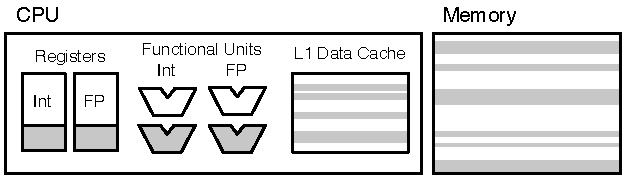
\includegraphics[width=\columnwidth]{figs/hwmodel.pdf}
      \caption{Hardware model assumed in our system. Shaded areas indicate
        components that support approximation.
        Registers and the data cache have SRAM storage cells that
        can be made approximate by decreasing supply voltage.
        Functional units support approximation via supply voltage
        reduction. Floating point functional units also support approximation
        via smaller
        mantissas. Main memory (DRAM) supports approximation by reducing
        refresh rate.\label{enerj:fig:hwmodel}}
\end{figure}

An instruction stream may have a mix of approximate and precise
instructions. Precise instructions have the same guarantees as
instructions in today's ISAs. Note that an approximate instruction is
simply a ``hint'' to the architecture that it may apply a variety of
energy-saving approximations when executing the given instruction. The
particular approximations employed by a given architecture are not
exposed to the program; a processor supporting no approximations just
executes approximate instructions precisely and saves no
energy. An approximation-aware ISA thus allows a single
binary to benefit from new approximations as they are
implemented in future microarchitectures.

\paragraph{Layout of approximate data.} Our hardware model supports
approximate memory data at a cache line granularity, in which software
can configure any line as approximate. This can be supported by having a
bit per line in each page that indicates whether the corresponding line is
approximate. Based on that bit, a cache controller determines
the supply voltage of a line (lower for approximate lines), and the
refresh rate for regions of DRAM\@. This bitmap needs to be kept
precise. With a typical cache line size of 64 bytes, this is less
than 0.2\% overhead. Note that both selective supply voltage for
caches~\cite{drowsycaches} and selective refresh rate for
DRAM~\cite{smartrefresh} are hardware techniques that have been
proposed in the past.

Setting approximation on a cache line basis requires the runtime
system to segregate approximate and precise data in different
cache lines. We propose the following simple
technique for laying out objects with both approximate and precise
fields. First, lay out the precise portion of the object (including
the \texttt{vtable} pointer) contiguously. Each cache line containing at least
one precise field is marked as precise. Then, lay out the approximate
fields after the end of the precise data. Some of this data may
be placed in a precise line (that is, a line containing some precise
data already); in this case, the approximate data stays precise and
saves no memory energy.
(Note that wasting space in the precise line in order to place the
data in an approximate line would use more memory and thus more
energy.)
The remaining approximate fields that do not
fit in the last precise line can be placed in approximate lines.

Fields in superclasses may not be reordered in subclasses.
Thus, a subclass of a class with approximate data may waste space in
an approximate line in order to place precise fields of the subclass
in a precise line.

While we simulate the artifacts of this layout scheme for our evaluation,
a finer granularity of approximate memory storage would mitigate or
eliminate the resulting loss of approximation.
More sophisticated layout algorithms could also improve energy savings;
this is a target for compile-time optimization.
Note that
even if an approximate field ends up stored in precise memory, it will
still be loaded into approximate registers and be subject to
approximate operations and algorithms.

The layout problem is much simpler for arrays of approximate primitive
types. The first line, which
contains the length and type information, must be precise, with all remaining
lines approximate.


\subsection{Hardware Techniques for Saving Energy }
\label{enerj:strategies}

% http://static.googleusercontent.com/external_content/untrusted_dlcp/research.google.com/en/us/archive/power_provisioning.pdf
%% Server
% processor: 80W, memory: 36W == ~ 54% total

%% smartphone
% http://ertos.nicta.com.au/publications/papers/Carroll_Heiser_10.pdf
% 16 cpu + 4 RAM == ~20% total. radio dominates.

%%laptop http://www.google.com/url?sa=t&source=web&cd=1&sqi=2&ved=0CBMQFjAA&url=http%3A%2F%2Fciteseerx.ist.psu.edu%2Fviewdoc%2Fdownload%3Fdoi%3D10.1.1.87.5604%26rep%3Drep1%26type%3Dpdf&ei=c5vPTMbRJIOisAPQloWqAw&usg=AFQjCNG8xSBDhqYtF9jopXkA80vVLnnEZQ


% http://www.eecs.umich.edu/~taustin/papers/TVLSI09-subliminal.pdf
% http://www.eecs.umich.edu/~taustin/papers/MICRO36-Razor.pdf
% http://passat.crhc.illinois.edu/rakeshk/hpca10_cam.pdf
There are many strategies for saving energy with approximate
storage and data operations. This section discusses some of the
techniques explored in prior research. We assume these techniques in
our simulations, which we describe later. The techniques are summarized
in Table~\ref{enerj:table:approximations}.


\paragraph{Voltage scaling in logic circuits.} Aggressive voltage
scaling can result in over $30\%$ energy reduction with
$\sim \! 1\%$ error rate~\cite{razor} and $22\%$ reduction with
$\sim \! 0.01\%$ error rate.  Recent work~\cite{hpca10cam,relax} proposed to
expose the errors to applications that can tolerate it and saw similar
results. In our model, we assume aggressive voltage scaling for the
processor units executing approximate instructions,
including integer and floating-point operations. As for an
error model, the choices are single bit flip, last value, and random
value. We consider all three but our evaluation mainly depicts the
random-value assumption, which is the most realistic.

\paragraph{Width reduction in floating point operations.}
A direct approach to approximate arithmetic operations on floating point values
is to ignore part of the mantissa in the operands. As observed in
\cite{bitwidthred}, many applications do not need the full mantissa.
According to their model,
a floating-point multiplier using 8-bit mantissas uses 78\% less
energy per operation than a full 24-bit multiplier.

% http://lca.ece.utexas.edu/pubs/isen_micro09.pdf
% leverages freed regions to lower refresh rate.

% http://www.cs.utah.edu/~rajeev/pubs/isca10.pdf

% ftp://ftp.computer.org/press/outgoing/proceedings/Patrick/ADI/sc10%20usb%20drive/data/0000a193.pdf

\paragraph{DRAM refresh rate.}
Reducing the refresh rate of dynamic RAM leads to potential data decay
but can substantially reduce power consumption with a low error rate.
As proposed by Liu et al.~\cite{flikker}, an approximation-aware DRAM system
might reduce the refresh rate on lines containing approximate data. As in
that work, we assume that reducing the refresh rate to 1~Hz
reduces power by about 20\%.
In a study performed by Bhalodia~\cite{dramthesis}, a DRAM cell not
refreshed for 10 seconds experiences a failure with per-bit
probability approximately $10^{-5}$. We conservatively assume this error
rate for the reduced refresh rate of 1~Hz.

\paragraph{SRAM supply voltage.}
Registers and data caches consist of static RAM (SRAM)
cells. Reducing the supply voltage to SRAM cells lowers the leakage
current of the cells but decreases the data integrity~\cite{drowsycaches}. As
examined by Kumar~\cite{sramthesis}, these
errors are dominated by \emph{read upsets} and \emph{write failures},
which occur when a bit is read or written. A read upset occurs when
the stored bit is flipped while it is read; a write failure occurs when the
wrong bit is written.
Reducing SRAM supply voltage by 80\% results in
read upset and write failure probabilities of $10^{-7.4}$ and
$10^{-4.94}$ respectively.
\emph{Soft failures}, bit flips in
stored data due to cosmic rays and other events, are comparatively
rare and depend less on the supply voltage.

\medskip
\noindent
Section~\ref{enerj:energymodel} describes the model we use to combine these
various potential energy savings into an overall CPU/memory system energy
reduction.
To put the potential energy savings in perspective, according to
recent studies~\cite{googlepower, aqeel}, the CPU and memory together account
for well over 50\% of the overall system power in servers as well as
notebooks. In a smartphone, CPU and memory account for about 20\% and
the radio typically close to 50\% of the overall
power~\cite{carroll2010}.


% uarch power breakdown -- server, PPro, old.
% http://www.eecs.harvard.edu/~dbrooks/isca2000.pdf
% cache: 12%, reg file: 23%, int unit: 15%, fp unit: 8%.


% http://cseweb.ucsd.edu/users/tullsen/micro09b.pdf
% http://www.cs.utexas.edu/~skeckler/pubs/islped03.ps


\begin{table}
\small
\begin{centering}
\begin{tabular}{ p{1.4in} c c c}
 & Mild & Medium & Aggressive \\
\hline \\[-2ex]
DRAM refresh: per-second bit flip probability
& $10^{-9}$ & $10^{-5}$ & $10^{-3}$ \\
Memory power saved
& 17\% & 22\% & 24\% \\[2ex]

SRAM read upset probability
& $10^{-16.7}$ & $10^{-7.4}$ & $10^{-3}$ \\
SRAM write failure probability
& $10^{-5.59}$ & $10^{-4.94}$ & $10^{-3}$ \\
Supply power saved
& 70\% & 80\% & 90\%* \\[2ex]

\texttt{float} mantissa bits
& $16$ & $8$ & $4$ \\
\texttt{double} mantissa bits
& $32$ & $16$ & $8$ \\
Energy saved per operation
& 32\% & 78\% & 85\%* \\[2ex]

Arithmetic timing error probability
& $10^{-6}$ & $10^{-4}$ & $10^{-2}$ \\
Energy saved per operation
& 12\%* & 22\% & 30\% \\
\end{tabular}

\end{centering}
\caption{Approximation strategies simulated in our evaluation.
Numbers marked with * are educated guesses by the authors; the others
are taken from the sources described in Section~\ref{enerj:strategies}. Note that
all values for the Medium level are taken from the literature.}
\label{enerj:table:approximations}
\end{table}




\section{Implementation}
\label{enerj:sec:impl}

We implement EnerJ as an extension to the Java
programming language based on the
pluggable type mechanism proposed by Papi et al.~\cite{pap2008}.
EnerJ is implemented using the
Checker Framework\footnote{\url{http://types.cs.washington.edu/checker-framework/}}
infrastructure,
which builds on the
JSR~308\footnote{\url{http://types.cs.washington.edu/jsr308/}}
extension to Java's annotation facility. JSR~308 permits annotations on
any explicit type in the program.
The EnerJ type checker extends the rules from Section~\ref{enerj:semantics} to all of
Java, including arrays and generics.
% WMD removed the following. We implemented more than just the rules
% in \ref{enerj:semantics}.
% We implement a checker that verifies the typing rules described in
% Section~\ref{enerj:semantics} using JSR~308's associated Checker Framework
% infrastructure.
% Turning off this footnote for now for anonymity, but we should put it
% back for the final version. --ALDS
% \footnote{Checker Framework:
% http://types.cs.washington.edu/checker-framework/}
We also implement a simulation infrastructure that emulates an
approximate computing architecture as described in Section~\ref{enerj:sec:execution}.
\footnote{The EnerJ type checker and simulator
are available from
our website:
\url{http://sampa.cs.washington.edu/sampa/EnerJ}
}

\subsection{Type Checker}
\label{enerj:checker}
EnerJ provides the type qualifiers listed
in Table~\ref{enerj:table:language}---\ilcode{@Approx}, \ilcode{@Precise},
\ilcode{@Top}, and \ilcode{@Context}---as JSR~308 type annotations.
The default type qualifier for unannotated types is \ilcode{@Precise}, meaning
that any Java program may be compiled as an EnerJ program with no change in
semantics. The programmer can add approximations to the
program incrementally.

% The \ilcode{@Approximable} annotation on classes is used by
% our type checker to decide the annotation of the \ilcode{this} reference.
% We decided to use the \ilcode{\_APPROX} naming convention to implement
% algorithmic approximation to stay compatible with JSR~308, which does
% not allow overloading methods that differ only in type qualifiers.

% ALDS: I'm not sure if this paragraph is necessary. First, we've already talked
% about why we need @Approximable and its discussion feels a little out of place
% here. Also, the _APPROX naming convention is not just because overloading on
% qualifiers is impossible: it's because we need to overload on the *receiver*
% type, which is not possible in general.

While reference types may be annotated as \ilcode{@Approx}, this only affects
the meaning of \ilcode{@Context} annotations in the class definition and
method binding on the receiver. Our implementation never
approximates pointers.
% \TODO{Don't we already say that somewhere? It seems strange here.}
% ALDS: It's an important implementation point that we never simulate any
% approximate storage or computation of pointers. It's implied by what's
% mentioned earlier, but it bears repeating here.


\subsection{Simulator}
To evaluate our system, we implement a compiler and runtime
system that executes EnerJ code as if it were running on an
approximation-aware architecture
as described in Section~\ref{enerj:sec:execution}. We instrument method calls,
object creation and destruction, arithmetic operators, and memory
accesses to collect statistics and inject faults.
The runtime system is implemented as a Java library and is invoked by the
instrumentation calls.
It records memory-footprint and arithmetic-operation statistics
while simultaneously injecting transient faults to emulate approximate
execution.

% strategies can be achieved with perfect granularity. For instance, we assume
% that the SRAM can store an approximate byte adjacent to a precise byte. In a
% real implementation of approximate hardware, coarser granularities of
% approximation may necessitate changes to memory layout as described on Section~\ref{enerj:sec:isa}, but this paper does not
% focus on such an implementation.
To avoid spurious errors due to approximation, our simulated
approximate functional units never raise divide-by-zero exceptions. Approximate
floating-point division by zero returns the NaN value;
approximate integer divide-by-zero returns zero.


% Maybe move this to future work.
% Aside from evaluating the feasibility of our system, this simulator would be
% useful as a testing tool for EnerJ applications. Because it simulates faults in
% software, it could (for instance) be used to test the limits of an application's
% error resilience by injecting faults far more frequently than would be
% realistic. The same technique could be applied to debugging for approximate
% applications. Similarly, the system could be used to prototype the tradeoffs
% involved in a proposed new hardware approximation.

\subsection{Approximations}
Our simulator implements the approximation strategies described in
Section~\ref{enerj:strategies}. Table~\ref{enerj:table:approximations} summarizes the
approximations used, their associated error probabilities, and their
estimated energy savings.

Floating-point bit-width reduction is performed when executing Java's
arithmetic operators on operands that are approximate \ilcode{float}
and \ilcode{double} values. SRAM read upsets and write failures are
simulated by flipping each bit read or written with a constant
probability. For DRAM refresh reduction, every bit also has an
independent probability of inversion; here, the probability is
proportional to the amount of time since the last access to the bit.

For the purposes of our evaluation, we distinguish SRAM and DRAM data using the
following rough approximation: data on the heap is considered to be stored
in DRAM; stack data is considered SRAM\@. Future evaluations not constrained by
the abstraction of the JVM could explore a more nuanced model.

\subsection{Energy Model}
\label{enerj:energymodel}
To summarize the effectiveness of EnerJ's energy-saving properties, we estimate
the potential overall savings of the processor/memory system when executing
each benchmark approximately. To do so, we consider a simplified model with
three components to the system's energy consumption: instruction execution,
SRAM storage (registers and cache), and DRAM storage.
Our model omits overheads of implementing or switching to approximate hardware.
For example, we do not model any latency in scaling the voltage on the logic
units. For this reason, our results can be considered optimistic; future work
should model approximate hardware in more detail.

To estimate the savings for instruction execution, we assign abstract energy
units to arithmetic operations. Integer operations take 37 units and floating point
operations take 40 units; of each of these, 22 units are consumed by the
instruction fetch and decode stage and may not be reduced by approximation
strategies. These estimations are based on three studies of architectural
power consumption~\cite{mcpat,burger2003,wattch}.
We calculate energy savings in instruction execution by scaling the
non-fetch, non-decode component of integer and floating-point instructions.

We assume that SRAM storage and instructions that access it account
for approximately 35\% of the microarchitecture's power consumption;
instruction execution logic consumes the remainder. To compute the
total CPU power savings, then, we scale the savings from SRAM storage
by 0.35 and the instruction power savings, described above, by 0.65.

Finally, we add the savings from DRAM storage to get an energy number for the
entire processor/memory system. For this, we consider a server-like setting,
where DRAM accounts for 45\% of the power and CPU 55\% \cite{googlepower}. Note
that in a mobile setting, memory consumes only 25\% of power so power savings in
the CPU will be more important \cite{carroll2010}.
% \TODO{At the end of Section 4 we have ``In a smartphone, CPU and
%  memory account for about 20\%'' and cite the same paper. This is
%  inconsistent or confusing.}
% ALDS: The earlier numbers were for CPU/memory relative to the full system.
% The current numbers are for memory relative to CPU/memory. I think this is
% pretty clear from the context (although admittedly not if you put the
% sentences side-by-side) -- but if you still think it needs clarifying, we can
% do something about it.

\section{Results}
\label{enerj:sec:res}

We evaluate EnerJ by annotating a variety of existing Java
programs. Table~\ref{enerj:table:applications} describes the applications we
used; they have been selected to be relevant in both mobile and server
settings. %, as energy is an important constraint in both
          %environments. %% Already said in intro.

\begin{table}
\small
\begin{center}

\begin{tabular}{l >{\raggedright}p{1.35in} >{\raggedright}p{1.25in} r r r r r}
& & & \multicolumn{1}{c}{Lines} & \multicolumn{1}{c}{Proportion} &
\multicolumn{1}{c}{Total} & \multicolumn{1}{c}{Annotated} &
\multicolumn{1}{c}{Endorse-} \tabularnewline
Application & Description & Error metric &
\multicolumn{1}{c}{of code} & \multicolumn{1}{c}{FP} &
\multicolumn{1}{c}{decls.} &
\multicolumn{1}{c}{decls.} & \multicolumn{1}{c}{ments} \tabularnewline
\hline
FFT & \multirow{5}{1.5in}{Scientific kernels from the SciMark2 benchmark} & Mean entry difference  & 168 & 38.2\% & 85 & 33\% & 2 \tabularnewline
SOR & & Mean entry difference  & 36 & 55.2\% & 28 & 25\% & 0 \tabularnewline
MonteCarlo & & Normalized difference  & 59 & 22.9\% & 15 & 20\% & 1 \tabularnewline
SparseMatMult & & Mean normalized difference  & 38 & 39.7\% & 29 & 14\% & 0 \tabularnewline
LU & & Mean entry difference  & 283 & 31.4\% & 150 & 23\% & 3 \tabularnewline[1.5ex]
ZXing & Smartphone bar code decoder & 1 if incorrect, 0 if correct  & 26171 & 1.7\% & 11506 & 4\% & 247 \tabularnewline
jMonkeyEngine & Mobile/desktop game engine & Fraction of correct decisions normalized to 0.5  & 5962 & 44.3\% & 2104 & 19\% & 63 \tabularnewline
ImageJ & Raster image manipulation & Mean pixel difference  & 156 & 0.0\% & 118 & 34\% & 18 \tabularnewline
Raytracer & 3D image renderer & Mean pixel difference  & 174 & 68.4\% & 92 & 33\% & 10 \tabularnewline
\end{tabular}

\vspace{-1ex}
\end{center}
\caption{Applications used in our evaluation,
application-specific metrics for quality of service, and
metrics of annotation density. ``Proportion FP''
indicates the percentage of dynamic arithmetic instructions observed that were
floating-point (as opposed to integer) operations.
}
\label{enerj:table:applications}
\end{table}

\paragraph{Applications.} We evaluate the FPU-heavy kernels of the SciMark2 benchmark suite to
reflect scientific workloads.\footnote{SciMark2:
  \url{http://math.nist.gov/scimark2/}} ZXing is a bar code reader library
targeted for mobile devices based on the Android operating
system.\footnote{ZXing: \url{http://code.google.com/p/zxing/}} Our workload
decodes QR Code two-dimensional bar code images. jMonkeyEngine is a 2D
and 3D game engine for both desktop and mobile
environments.\footnote{jMonkeyEngine: \url{http://www.jmonkeyengine.com/}}
We run a workload that consists of many 3D triangle intersection
problems, an algorithm frequently used for collision detection in
games.

ImageJ is an image-manipulation program; our workload executes a flood fill
operation.\footnote{ImageJ: \url{http://rsbweb.nih.gov/ij/}} This workload was
selected as representative of error-resilient algorithms with primarily
integer---rather than floating point---data.
Because the code already includes extensive
safety precautions such as bounds checking, our annotation for ImageJ is
extremely aggressive: even pixel coordinates are marked as approximate.
Raytracer is a simple 3D renderer; our workload executes
ray plane intersection on a simple scene.\footnote{Raytracer:
\url{http://www.planet-source-code.com/vb/scripts/ShowCode.asp?txtCodeId=5590&lngWId=2}}

\paragraph{Annotation approach.} We annotated each application
manually. While many possible
annotations exist for a given program, we attempted to strike a
balance between reliability and energy savings. As a rule, however, we
attempted to annotate the programs in a way that never causes
them to crash (or throw an unhandled exception); it is important to
show that EnerJ allows programmers to write approximate programs that
never fail catastrophically. In our experiments, each benchmark produces
an output on every run. This is in contrast to approximation techniques
that do not attempt to prevent crashes \cite{flikker, wong-selse06, li07}.
Naturally, we focused our effort on code where most of the
time is spent.
% ALDS: Past tense is appropriate for procedural descriptions.

Three of the authors ported the applications used in our
evaluation. In every case, we were unfamiliar with the codebase
beforehand, so our annotations did not depend on extensive domain
knowledge. The annotations were not labor intensive.


\paragraph{QoS metrics.} For each application, we measure the
degradation in output quality of approximate executions with respect
to the precise executions. To do so, we define application-specific
quality of service (QoS) metrics. Defining our own ad-hoc QoS metrics
is necessary to compare output degradation across applications.
A number of similar studies of
application-level tolerance to transient faults have also taken this
approach \cite{qosprof, green, dekruijf-selse09, ersa, wong-selse06,
  softcomputing}. The third column in
Table~\ref{enerj:table:applications} shows our metric for each application.

Output error ranges from $0$ (indicating output identical to the
precise version) to $1$ (indicating completely meaningless output). For
applications that produce lists of numbers (e.g., SparseMatMult's output
matrix), we compute the error as the mean entry-wise difference between the
pristine output and the degraded output. Each numerical difference is limited
by $1$, so if an entry in the output is \ilcode{NaN},
that entry contributes an error of $1$. For benchmarks where the output is not
numeric (i.e., ZXing, which outputs a string), the error is $0$ when the output
is correct and $1$ otherwise. %when it is incorrect.


\subsection{Energy Savings}

\begin{figure}
% Created by tikzDevice version 0.5.2 on 2011-03-14 15:14:42
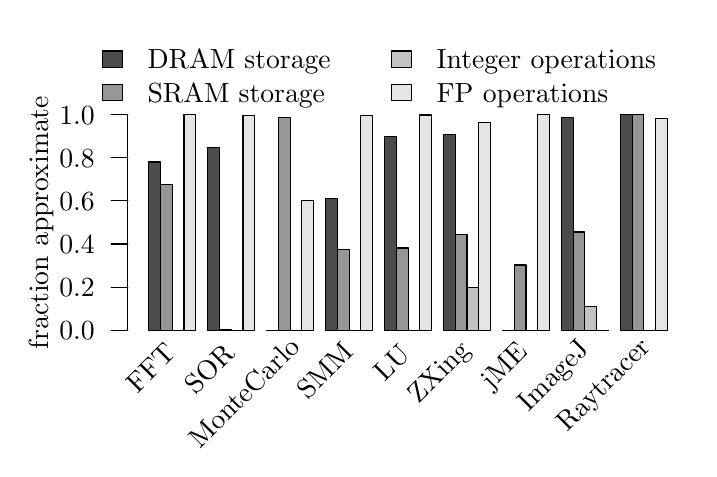
\begin{tikzpicture}[x=1pt,y=1pt]
\draw[color=white,opacity=0] (0,0) rectangle (238.49,151.77);
\begin{scope}
\path[clip] (  0.00,  0.00) rectangle (238.49,151.77);
\definecolor[named]{drawColor}{rgb}{0.18,0.00,0.42}
\definecolor[named]{fillColor}{rgb}{0.45,0.45,0.18}
\definecolor[named]{drawColor}{rgb}{0.00,0.00,0.00}
\definecolor[named]{fillColor}{rgb}{0.30,0.30,0.30}

\draw[color=drawColor,line cap=round,line join=round,fill=fillColor,] ( 43.50, 42.60) rectangle ( 47.76,103.42);
\definecolor[named]{fillColor}{rgb}{0.59,0.59,0.59}

\draw[color=drawColor,line cap=round,line join=round,fill=fillColor,] ( 47.76, 42.60) rectangle ( 52.02, 95.34);
\definecolor[named]{fillColor}{rgb}{0.76,0.76,0.76}

\draw[color=drawColor,line cap=round,line join=round,fill=fillColor,] ( 52.02, 42.60) rectangle ( 56.28, 42.60);
\definecolor[named]{fillColor}{rgb}{0.90,0.90,0.90}

\draw[color=drawColor,line cap=round,line join=round,fill=fillColor,] ( 56.28, 42.60) rectangle ( 60.54,120.53);
\definecolor[named]{fillColor}{rgb}{0.30,0.30,0.30}

\draw[color=drawColor,line cap=round,line join=round,fill=fillColor,] ( 64.81, 42.60) rectangle ( 69.07,108.72);
\definecolor[named]{fillColor}{rgb}{0.59,0.59,0.59}

\draw[color=drawColor,line cap=round,line join=round,fill=fillColor,] ( 69.07, 42.60) rectangle ( 73.33, 42.71);
\definecolor[named]{fillColor}{rgb}{0.76,0.76,0.76}

\draw[color=drawColor,line cap=round,line join=round,fill=fillColor,] ( 73.33, 42.60) rectangle ( 77.59, 42.60);
\definecolor[named]{fillColor}{rgb}{0.90,0.90,0.90}

\draw[color=drawColor,line cap=round,line join=round,fill=fillColor,] ( 77.59, 42.60) rectangle ( 81.85,120.36);
\definecolor[named]{fillColor}{rgb}{0.30,0.30,0.30}

\draw[color=drawColor,line cap=round,line join=round,fill=fillColor,] ( 86.11, 42.60) rectangle ( 90.37, 42.60);
\definecolor[named]{fillColor}{rgb}{0.59,0.59,0.59}

\draw[color=drawColor,line cap=round,line join=round,fill=fillColor,] ( 90.37, 42.60) rectangle ( 94.63,119.67);
\definecolor[named]{fillColor}{rgb}{0.76,0.76,0.76}

\draw[color=drawColor,line cap=round,line join=round,fill=fillColor,] ( 94.63, 42.60) rectangle ( 98.89, 42.60);
\definecolor[named]{fillColor}{rgb}{0.90,0.90,0.90}

\draw[color=drawColor,line cap=round,line join=round,fill=fillColor,] ( 98.89, 42.60) rectangle (103.16, 89.36);
\definecolor[named]{fillColor}{rgb}{0.30,0.30,0.30}

\draw[color=drawColor,line cap=round,line join=round,fill=fillColor,] (107.42, 42.60) rectangle (111.68, 90.22);
\definecolor[named]{fillColor}{rgb}{0.59,0.59,0.59}

\draw[color=drawColor,line cap=round,line join=round,fill=fillColor,] (111.68, 42.60) rectangle (115.94, 71.94);
\definecolor[named]{fillColor}{rgb}{0.76,0.76,0.76}

\draw[color=drawColor,line cap=round,line join=round,fill=fillColor,] (115.94, 42.60) rectangle (120.20, 42.60);
\definecolor[named]{fillColor}{rgb}{0.90,0.90,0.90}

\draw[color=drawColor,line cap=round,line join=round,fill=fillColor,] (120.20, 42.60) rectangle (124.46,120.09);
\definecolor[named]{fillColor}{rgb}{0.30,0.30,0.30}

\draw[color=drawColor,line cap=round,line join=round,fill=fillColor,] (128.72, 42.60) rectangle (132.98,112.64);
\definecolor[named]{fillColor}{rgb}{0.59,0.59,0.59}

\draw[color=drawColor,line cap=round,line join=round,fill=fillColor,] (132.98, 42.60) rectangle (137.25, 72.35);
\definecolor[named]{fillColor}{rgb}{0.76,0.76,0.76}

\draw[color=drawColor,line cap=round,line join=round,fill=fillColor,] (137.25, 42.60) rectangle (141.51, 42.60);
\definecolor[named]{fillColor}{rgb}{0.90,0.90,0.90}

\draw[color=drawColor,line cap=round,line join=round,fill=fillColor,] (141.51, 42.60) rectangle (145.77,120.43);
\definecolor[named]{fillColor}{rgb}{0.30,0.30,0.30}

\draw[color=drawColor,line cap=round,line join=round,fill=fillColor,] (150.03, 42.60) rectangle (154.29,113.43);
\definecolor[named]{fillColor}{rgb}{0.59,0.59,0.59}

\draw[color=drawColor,line cap=round,line join=round,fill=fillColor,] (154.29, 42.60) rectangle (158.55, 77.24);
\definecolor[named]{fillColor}{rgb}{0.76,0.76,0.76}

\draw[color=drawColor,line cap=round,line join=round,fill=fillColor,] (158.55, 42.60) rectangle (162.81, 57.99);
\definecolor[named]{fillColor}{rgb}{0.90,0.90,0.90}

\draw[color=drawColor,line cap=round,line join=round,fill=fillColor,] (162.81, 42.60) rectangle (167.07,117.78);
\definecolor[named]{fillColor}{rgb}{0.30,0.30,0.30}

\draw[color=drawColor,line cap=round,line join=round,fill=fillColor,] (171.33, 42.60) rectangle (175.60, 42.66);
\definecolor[named]{fillColor}{rgb}{0.59,0.59,0.59}

\draw[color=drawColor,line cap=round,line join=round,fill=fillColor,] (175.60, 42.60) rectangle (179.86, 66.20);
\definecolor[named]{fillColor}{rgb}{0.76,0.76,0.76}

\draw[color=drawColor,line cap=round,line join=round,fill=fillColor,] (179.86, 42.60) rectangle (184.12, 42.60);
\definecolor[named]{fillColor}{rgb}{0.90,0.90,0.90}

\draw[color=drawColor,line cap=round,line join=round,fill=fillColor,] (184.12, 42.60) rectangle (188.38,120.57);
\definecolor[named]{fillColor}{rgb}{0.30,0.30,0.30}

\draw[color=drawColor,line cap=round,line join=round,fill=fillColor,] (192.64, 42.60) rectangle (196.90,119.37);
\definecolor[named]{fillColor}{rgb}{0.59,0.59,0.59}

\draw[color=drawColor,line cap=round,line join=round,fill=fillColor,] (196.90, 42.60) rectangle (201.16, 78.13);
\definecolor[named]{fillColor}{rgb}{0.76,0.76,0.76}

\draw[color=drawColor,line cap=round,line join=round,fill=fillColor,] (201.16, 42.60) rectangle (205.42, 51.17);
\definecolor[named]{fillColor}{rgb}{0.90,0.90,0.90}

\draw[color=drawColor,line cap=round,line join=round,fill=fillColor,] (205.42, 42.60) rectangle (209.69, 42.60);
\definecolor[named]{fillColor}{rgb}{0.30,0.30,0.30}

\draw[color=drawColor,line cap=round,line join=round,fill=fillColor,] (213.95, 42.60) rectangle (218.21,120.55);
\definecolor[named]{fillColor}{rgb}{0.59,0.59,0.59}

\draw[color=drawColor,line cap=round,line join=round,fill=fillColor,] (218.21, 42.60) rectangle (222.47,120.56);
\definecolor[named]{fillColor}{rgb}{0.76,0.76,0.76}

\draw[color=drawColor,line cap=round,line join=round,fill=fillColor,] (222.47, 42.60) rectangle (226.73, 42.60);
\definecolor[named]{fillColor}{rgb}{0.90,0.90,0.90}

\draw[color=drawColor,line cap=round,line join=round,fill=fillColor,] (226.73, 42.60) rectangle (230.99,119.07);
\end{scope}
\begin{scope}
\path[clip] (  0.00,  0.00) rectangle (238.49,151.77);
\definecolor[named]{drawColor}{rgb}{0.18,0.00,0.42}
\definecolor[named]{fillColor}{rgb}{0.45,0.45,0.18}
\definecolor[named]{drawColor}{rgb}{0.00,0.00,0.00}

\draw[color=drawColor,line cap=round,line join=round,fill opacity=0.00,] ( 36.00, 42.60) -- ( 36.00,120.57);

\draw[color=drawColor,line cap=round,line join=round,fill opacity=0.00,] ( 36.00, 42.60) -- ( 30.00, 42.60);

\draw[color=drawColor,line cap=round,line join=round,fill opacity=0.00,] ( 36.00, 58.19) -- ( 30.00, 58.19);

\draw[color=drawColor,line cap=round,line join=round,fill opacity=0.00,] ( 36.00, 73.79) -- ( 30.00, 73.79);

\draw[color=drawColor,line cap=round,line join=round,fill opacity=0.00,] ( 36.00, 89.38) -- ( 30.00, 89.38);

\draw[color=drawColor,line cap=round,line join=round,fill opacity=0.00,] ( 36.00,104.97) -- ( 30.00,104.97);

\draw[color=drawColor,line cap=round,line join=round,fill opacity=0.00,] ( 36.00,120.57) -- ( 30.00,120.57);

\node[color=drawColor,anchor=base east,inner sep=0pt, outer sep=0pt, scale=  1.00] at ( 24.00, 39.16) {0.0%
};

\node[color=drawColor,anchor=base east,inner sep=0pt, outer sep=0pt, scale=  1.00] at ( 24.00, 54.75) {0.2%
};

\node[color=drawColor,anchor=base east,inner sep=0pt, outer sep=0pt, scale=  1.00] at ( 24.00, 70.34) {0.4%
};

\node[color=drawColor,anchor=base east,inner sep=0pt, outer sep=0pt, scale=  1.00] at ( 24.00, 85.94) {0.6%
};

\node[color=drawColor,anchor=base east,inner sep=0pt, outer sep=0pt, scale=  1.00] at ( 24.00,101.53) {0.8%
};

\node[color=drawColor,anchor=base east,inner sep=0pt, outer sep=0pt, scale=  1.00] at ( 24.00,117.12) {1.0%
};

\node[rotate= 90.00,color=drawColor,anchor=base,inner sep=0pt, outer sep=0pt, scale=  1.00] at (  7.20, 81.58) {fraction approximate%
};
\end{scope}
\begin{scope}
\path[clip] (  0.00,  0.00) rectangle (238.49,151.77);
\definecolor[named]{drawColor}{rgb}{0.18,0.00,0.42}
\definecolor[named]{fillColor}{rgb}{0.45,0.45,0.18}
\definecolor[named]{drawColor}{rgb}{0.00,0.00,0.00}
\definecolor[named]{fillColor}{rgb}{0.30,0.30,0.30}

\draw[color=drawColor,line cap=round,line join=round,fill=fillColor,] ( 26.93,143.53) rectangle ( 34.13,137.53);
\definecolor[named]{fillColor}{rgb}{0.59,0.59,0.59}

\draw[color=drawColor,line cap=round,line join=round,fill=fillColor,] ( 26.93,131.53) rectangle ( 34.13,125.53);
\definecolor[named]{fillColor}{rgb}{0.76,0.76,0.76}

\draw[color=drawColor,line cap=round,line join=round,fill=fillColor,] (131.39,143.53) rectangle (138.59,137.53);
\definecolor[named]{fillColor}{rgb}{0.90,0.90,0.90}

\draw[color=drawColor,line cap=round,line join=round,fill=fillColor,] (131.39,131.53) rectangle (138.59,125.53);

\node[color=drawColor,anchor=base west,inner sep=0pt, outer sep=0pt, scale=  1.00] at ( 43.13,137.09) {DRAM storage%
};

\node[color=drawColor,anchor=base west,inner sep=0pt, outer sep=0pt, scale=  1.00] at ( 43.13,125.09) {SRAM storage%
};

\node[color=drawColor,anchor=base west,inner sep=0pt, outer sep=0pt, scale=  1.00] at (147.59,137.09) {Integer operations%
};

\node[color=drawColor,anchor=base west,inner sep=0pt, outer sep=0pt, scale=  1.00] at (147.59,125.09) {FP operations%
};

\node[rotate= 45.00,color=drawColor,anchor=base east,inner sep=0pt, outer sep=0pt, scale=  1.00] at ( 53.76, 33.80) {FFT%
};

\node[rotate= 45.00,color=drawColor,anchor=base east,inner sep=0pt, outer sep=0pt, scale=  1.00] at ( 75.10, 33.83) {SOR%
};

\node[rotate= 45.00,color=drawColor,anchor=base east,inner sep=0pt, outer sep=0pt, scale=  1.00] at ( 98.59, 36.02) {MonteCarlo%
};

\node[rotate= 45.00,color=drawColor,anchor=base east,inner sep=0pt, outer sep=0pt, scale=  1.00] at (117.93, 34.06) {SMM%
};

\node[rotate= 45.00,color=drawColor,anchor=base east,inner sep=0pt, outer sep=0pt, scale=  1.00] at (138.52, 33.34) {LU%
};

\node[rotate= 45.00,color=drawColor,anchor=base east,inner sep=0pt, outer sep=0pt, scale=  1.00] at (160.07, 34.96) {ZXing%
};

\node[rotate= 45.00,color=drawColor,anchor=base east,inner sep=0pt, outer sep=0pt, scale=  1.00] at (180.82, 34.40) {jME%
};

\node[rotate= 45.00,color=drawColor,anchor=base east,inner sep=0pt, outer sep=0pt, scale=  1.00] at (203.01, 35.28) {ImageJ%
};

\node[rotate= 45.00,color=drawColor,anchor=base east,inner sep=0pt, outer sep=0pt, scale=  1.00] at (225.12, 36.09) {Raytracer%
};
\end{scope}
\end{tikzpicture}

\vspace{-4ex} % mysterious gap\
\caption{Proportion of approximate storage and computation in each benchmark.
For storage (SRAM and DRAM) measurements, the bars
show the fraction of byte-seconds used in storing approximate data.
For functional unit operations, we show the fraction of dynamic operations
that were executed approximately.}
\label{enerj:fig:approximateness}
\end{figure}

\begin{figure}
% Created by tikzDevice version 0.6.2 on 2012-11-10 18:33:02
% !TEX encoding = UTF-8 Unicode
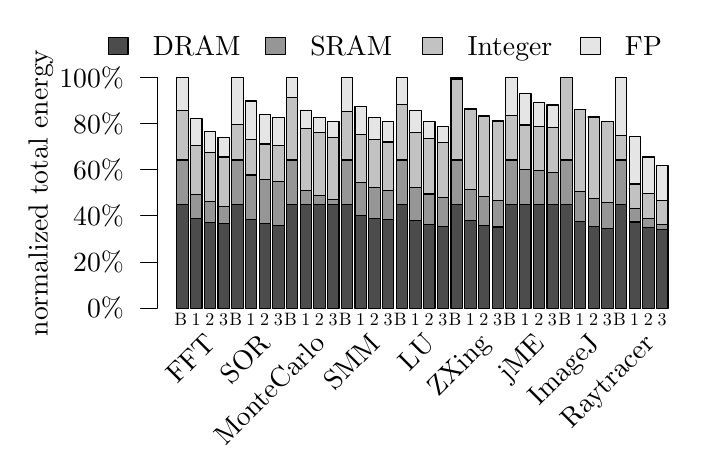
\begin{tikzpicture}[x=1pt,y=1pt]
\definecolor[named]{drawColor}{rgb}{0.00,0.00,0.00}
\definecolor[named]{fillColor}{rgb}{1.00,1.00,1.00}
\fill[color=fillColor,fill opacity=0.00,] (0,0) rectangle (238.49,151.77);
\begin{scope}
\path[clip] (  0.00,  0.00) rectangle (238.49,151.77);
\definecolor[named]{drawColor}{rgb}{0.00,0.00,0.00}
\definecolor[named]{fillColor}{rgb}{0.30,0.30,0.30}

\draw[color=drawColor,line cap=round,line join=round,fill=fillColor,] ( 53.90, 50.40) rectangle ( 58.03, 87.92);
\definecolor[named]{fillColor}{rgb}{0.59,0.59,0.59}

\draw[color=drawColor,line cap=round,line join=round,fill=fillColor,] ( 53.90, 87.92) rectangle ( 58.03,103.96);
\definecolor[named]{fillColor}{rgb}{0.76,0.76,0.76}

\draw[color=drawColor,line cap=round,line join=round,fill=fillColor,] ( 53.90,103.96) rectangle ( 58.03,121.82);
\definecolor[named]{fillColor}{rgb}{0.90,0.90,0.90}

\draw[color=drawColor,line cap=round,line join=round,fill=fillColor,] ( 53.90,121.82) rectangle ( 58.03,133.77);
\definecolor[named]{fillColor}{rgb}{0.30,0.30,0.30}

\draw[color=drawColor,line cap=round,line join=round,fill=fillColor,] ( 58.85, 50.40) rectangle ( 62.98, 82.94);
\definecolor[named]{fillColor}{rgb}{0.59,0.59,0.59}

\draw[color=drawColor,line cap=round,line join=round,fill=fillColor,] ( 58.85, 82.94) rectangle ( 62.98, 91.39);
\definecolor[named]{fillColor}{rgb}{0.76,0.76,0.76}

\draw[color=drawColor,line cap=round,line join=round,fill=fillColor,] ( 58.85, 91.39) rectangle ( 62.98,109.24);
\definecolor[named]{fillColor}{rgb}{0.90,0.90,0.90}

\draw[color=drawColor,line cap=round,line join=round,fill=fillColor,] ( 58.85,109.24) rectangle ( 62.98,119.03);
\definecolor[named]{fillColor}{rgb}{0.30,0.30,0.30}

\draw[color=drawColor,line cap=round,line join=round,fill=fillColor,] ( 63.81, 50.40) rectangle ( 67.93, 81.48);
\definecolor[named]{fillColor}{rgb}{0.59,0.59,0.59}

\draw[color=drawColor,line cap=round,line join=round,fill=fillColor,] ( 63.81, 81.48) rectangle ( 67.93, 88.84);
\definecolor[named]{fillColor}{rgb}{0.76,0.76,0.76}

\draw[color=drawColor,line cap=round,line join=round,fill=fillColor,] ( 63.81, 88.84) rectangle ( 67.93,106.70);
\definecolor[named]{fillColor}{rgb}{0.90,0.90,0.90}

\draw[color=drawColor,line cap=round,line join=round,fill=fillColor,] ( 63.81,106.70) rectangle ( 67.93,114.19);
\definecolor[named]{fillColor}{rgb}{0.30,0.30,0.30}

\draw[color=drawColor,line cap=round,line join=round,fill=fillColor,] ( 68.76, 50.40) rectangle ( 72.89, 80.89);
\definecolor[named]{fillColor}{rgb}{0.59,0.59,0.59}

\draw[color=drawColor,line cap=round,line join=round,fill=fillColor,] ( 68.76, 80.89) rectangle ( 72.89, 87.17);
\definecolor[named]{fillColor}{rgb}{0.76,0.76,0.76}

\draw[color=drawColor,line cap=round,line join=round,fill=fillColor,] ( 68.76, 87.17) rectangle ( 72.89,105.02);
\definecolor[named]{fillColor}{rgb}{0.90,0.90,0.90}

\draw[color=drawColor,line cap=round,line join=round,fill=fillColor,] ( 68.76,105.02) rectangle ( 72.89,112.16);
\definecolor[named]{fillColor}{rgb}{0.30,0.30,0.30}

\draw[color=drawColor,line cap=round,line join=round,fill=fillColor,] ( 73.71, 50.40) rectangle ( 77.84, 87.92);
\definecolor[named]{fillColor}{rgb}{0.59,0.59,0.59}

\draw[color=drawColor,line cap=round,line join=round,fill=fillColor,] ( 73.71, 87.92) rectangle ( 77.84,103.96);
\definecolor[named]{fillColor}{rgb}{0.76,0.76,0.76}

\draw[color=drawColor,line cap=round,line join=round,fill=fillColor,] ( 73.71,103.96) rectangle ( 77.84,116.73);
\definecolor[named]{fillColor}{rgb}{0.90,0.90,0.90}

\draw[color=drawColor,line cap=round,line join=round,fill=fillColor,] ( 73.71,116.73) rectangle ( 77.84,133.77);
\definecolor[named]{fillColor}{rgb}{0.30,0.30,0.30}

\draw[color=drawColor,line cap=round,line join=round,fill=fillColor,] ( 78.67, 50.40) rectangle ( 82.79, 82.51);
\definecolor[named]{fillColor}{rgb}{0.59,0.59,0.59}

\draw[color=drawColor,line cap=round,line join=round,fill=fillColor,] ( 78.67, 82.51) rectangle ( 82.79, 98.54);
\definecolor[named]{fillColor}{rgb}{0.76,0.76,0.76}

\draw[color=drawColor,line cap=round,line join=round,fill=fillColor,] ( 78.67, 98.54) rectangle ( 82.79,111.31);
\definecolor[named]{fillColor}{rgb}{0.90,0.90,0.90}

\draw[color=drawColor,line cap=round,line join=round,fill=fillColor,] ( 78.67,111.31) rectangle ( 82.79,125.27);
\definecolor[named]{fillColor}{rgb}{0.30,0.30,0.30}

\draw[color=drawColor,line cap=round,line join=round,fill=fillColor,] ( 83.62, 50.40) rectangle ( 87.75, 80.92);
\definecolor[named]{fillColor}{rgb}{0.59,0.59,0.59}

\draw[color=drawColor,line cap=round,line join=round,fill=fillColor,] ( 83.62, 80.92) rectangle ( 87.75, 96.95);
\definecolor[named]{fillColor}{rgb}{0.76,0.76,0.76}

\draw[color=drawColor,line cap=round,line join=round,fill=fillColor,] ( 83.62, 96.95) rectangle ( 87.75,109.72);
\definecolor[named]{fillColor}{rgb}{0.90,0.90,0.90}

\draw[color=drawColor,line cap=round,line join=round,fill=fillColor,] ( 83.62,109.72) rectangle ( 87.75,120.42);
\definecolor[named]{fillColor}{rgb}{0.30,0.30,0.30}

\draw[color=drawColor,line cap=round,line join=round,fill=fillColor,] ( 88.57, 50.40) rectangle ( 92.70, 80.28);
\definecolor[named]{fillColor}{rgb}{0.59,0.59,0.59}

\draw[color=drawColor,line cap=round,line join=round,fill=fillColor,] ( 88.57, 80.28) rectangle ( 92.70, 96.31);
\definecolor[named]{fillColor}{rgb}{0.76,0.76,0.76}

\draw[color=drawColor,line cap=round,line join=round,fill=fillColor,] ( 88.57, 96.31) rectangle ( 92.70,109.08);
\definecolor[named]{fillColor}{rgb}{0.90,0.90,0.90}

\draw[color=drawColor,line cap=round,line join=round,fill=fillColor,] ( 88.57,109.08) rectangle ( 92.70,119.27);
\definecolor[named]{fillColor}{rgb}{0.30,0.30,0.30}

\draw[color=drawColor,line cap=round,line join=round,fill=fillColor,] ( 93.53, 50.40) rectangle ( 97.65, 87.92);
\definecolor[named]{fillColor}{rgb}{0.59,0.59,0.59}

\draw[color=drawColor,line cap=round,line join=round,fill=fillColor,] ( 93.53, 87.92) rectangle ( 97.65,103.96);
\definecolor[named]{fillColor}{rgb}{0.76,0.76,0.76}

\draw[color=drawColor,line cap=round,line join=round,fill=fillColor,] ( 93.53,103.96) rectangle ( 97.65,126.52);
\definecolor[named]{fillColor}{rgb}{0.90,0.90,0.90}

\draw[color=drawColor,line cap=round,line join=round,fill=fillColor,] ( 93.53,126.52) rectangle ( 97.65,133.77);
\definecolor[named]{fillColor}{rgb}{0.30,0.30,0.30}

\draw[color=drawColor,line cap=round,line join=round,fill=fillColor,] ( 98.48, 50.40) rectangle (102.61, 87.92);
\definecolor[named]{fillColor}{rgb}{0.59,0.59,0.59}

\draw[color=drawColor,line cap=round,line join=round,fill=fillColor,] ( 98.48, 87.92) rectangle (102.61, 92.86);
\definecolor[named]{fillColor}{rgb}{0.76,0.76,0.76}

\draw[color=drawColor,line cap=round,line join=round,fill=fillColor,] ( 98.48, 92.86) rectangle (102.61,115.41);
\definecolor[named]{fillColor}{rgb}{0.90,0.90,0.90}

\draw[color=drawColor,line cap=round,line join=round,fill=fillColor,] ( 98.48,115.41) rectangle (102.61,121.88);
\definecolor[named]{fillColor}{rgb}{0.30,0.30,0.30}

\draw[color=drawColor,line cap=round,line join=round,fill=fillColor,] (103.43, 50.40) rectangle (107.56, 87.92);
\definecolor[named]{fillColor}{rgb}{0.59,0.59,0.59}

\draw[color=drawColor,line cap=round,line join=round,fill=fillColor,] (103.43, 87.92) rectangle (107.56, 91.27);
\definecolor[named]{fillColor}{rgb}{0.76,0.76,0.76}

\draw[color=drawColor,line cap=round,line join=round,fill=fillColor,] (103.43, 91.27) rectangle (107.56,113.83);
\definecolor[named]{fillColor}{rgb}{0.90,0.90,0.90}

\draw[color=drawColor,line cap=round,line join=round,fill=fillColor,] (103.43,113.83) rectangle (107.56,119.45);
\definecolor[named]{fillColor}{rgb}{0.30,0.30,0.30}

\draw[color=drawColor,line cap=round,line join=round,fill=fillColor,] (108.39, 50.40) rectangle (112.51, 87.92);
\definecolor[named]{fillColor}{rgb}{0.59,0.59,0.59}

\draw[color=drawColor,line cap=round,line join=round,fill=fillColor,] (108.39, 87.92) rectangle (112.51, 89.69);
\definecolor[named]{fillColor}{rgb}{0.76,0.76,0.76}

\draw[color=drawColor,line cap=round,line join=round,fill=fillColor,] (108.39, 89.69) rectangle (112.51,112.24);
\definecolor[named]{fillColor}{rgb}{0.90,0.90,0.90}

\draw[color=drawColor,line cap=round,line join=round,fill=fillColor,] (108.39,112.24) rectangle (112.51,117.74);
\definecolor[named]{fillColor}{rgb}{0.30,0.30,0.30}

\draw[color=drawColor,line cap=round,line join=round,fill=fillColor,] (113.34, 50.40) rectangle (117.47, 87.92);
\definecolor[named]{fillColor}{rgb}{0.59,0.59,0.59}

\draw[color=drawColor,line cap=round,line join=round,fill=fillColor,] (113.34, 87.92) rectangle (117.47,103.96);
\definecolor[named]{fillColor}{rgb}{0.76,0.76,0.76}

\draw[color=drawColor,line cap=round,line join=round,fill=fillColor,] (113.34,103.96) rectangle (117.47,121.39);
\definecolor[named]{fillColor}{rgb}{0.90,0.90,0.90}

\draw[color=drawColor,line cap=round,line join=round,fill=fillColor,] (113.34,121.39) rectangle (117.47,133.77);
\definecolor[named]{fillColor}{rgb}{0.30,0.30,0.30}

\draw[color=drawColor,line cap=round,line join=round,fill=fillColor,] (118.29, 50.40) rectangle (122.42, 84.02);
\definecolor[named]{fillColor}{rgb}{0.59,0.59,0.59}

\draw[color=drawColor,line cap=round,line join=round,fill=fillColor,] (118.29, 84.02) rectangle (122.42, 95.84);
\definecolor[named]{fillColor}{rgb}{0.76,0.76,0.76}

\draw[color=drawColor,line cap=round,line join=round,fill=fillColor,] (118.29, 95.84) rectangle (122.42,113.27);
\definecolor[named]{fillColor}{rgb}{0.90,0.90,0.90}

\draw[color=drawColor,line cap=round,line join=round,fill=fillColor,] (118.29,113.27) rectangle (122.42,123.42);
\definecolor[named]{fillColor}{rgb}{0.30,0.30,0.30}

\draw[color=drawColor,line cap=round,line join=round,fill=fillColor,] (123.25, 50.40) rectangle (127.37, 82.87);
\definecolor[named]{fillColor}{rgb}{0.59,0.59,0.59}

\draw[color=drawColor,line cap=round,line join=round,fill=fillColor,] (123.25, 82.87) rectangle (127.37, 94.09);
\definecolor[named]{fillColor}{rgb}{0.76,0.76,0.76}

\draw[color=drawColor,line cap=round,line join=round,fill=fillColor,] (123.25, 94.09) rectangle (127.37,111.52);
\definecolor[named]{fillColor}{rgb}{0.90,0.90,0.90}

\draw[color=drawColor,line cap=round,line join=round,fill=fillColor,] (123.25,111.52) rectangle (127.37,119.31);
\definecolor[named]{fillColor}{rgb}{0.30,0.30,0.30}

\draw[color=drawColor,line cap=round,line join=round,fill=fillColor,] (128.20, 50.40) rectangle (132.33, 82.42);
\definecolor[named]{fillColor}{rgb}{0.59,0.59,0.59}

\draw[color=drawColor,line cap=round,line join=round,fill=fillColor,] (128.20, 82.42) rectangle (132.33, 93.03);
\definecolor[named]{fillColor}{rgb}{0.76,0.76,0.76}

\draw[color=drawColor,line cap=round,line join=round,fill=fillColor,] (128.20, 93.03) rectangle (132.33,110.45);
\definecolor[named]{fillColor}{rgb}{0.90,0.90,0.90}

\draw[color=drawColor,line cap=round,line join=round,fill=fillColor,] (128.20,110.45) rectangle (132.33,117.88);
\definecolor[named]{fillColor}{rgb}{0.30,0.30,0.30}

\draw[color=drawColor,line cap=round,line join=round,fill=fillColor,] (133.15, 50.40) rectangle (137.28, 87.92);
\definecolor[named]{fillColor}{rgb}{0.59,0.59,0.59}

\draw[color=drawColor,line cap=round,line join=round,fill=fillColor,] (133.15, 87.92) rectangle (137.28,103.96);
\definecolor[named]{fillColor}{rgb}{0.76,0.76,0.76}

\draw[color=drawColor,line cap=round,line join=round,fill=fillColor,] (133.15,103.96) rectangle (137.28,123.89);
\definecolor[named]{fillColor}{rgb}{0.90,0.90,0.90}

\draw[color=drawColor,line cap=round,line join=round,fill=fillColor,] (133.15,123.89) rectangle (137.28,133.77);
\definecolor[named]{fillColor}{rgb}{0.30,0.30,0.30}

\draw[color=drawColor,line cap=round,line join=round,fill=fillColor,] (138.11, 50.40) rectangle (142.23, 82.19);
\definecolor[named]{fillColor}{rgb}{0.59,0.59,0.59}

\draw[color=drawColor,line cap=round,line join=round,fill=fillColor,] (138.11, 82.19) rectangle (142.23, 93.95);
\definecolor[named]{fillColor}{rgb}{0.76,0.76,0.76}

\draw[color=drawColor,line cap=round,line join=round,fill=fillColor,] (138.11, 93.95) rectangle (142.23,113.87);
\definecolor[named]{fillColor}{rgb}{0.90,0.90,0.90}

\draw[color=drawColor,line cap=round,line join=round,fill=fillColor,] (138.11,113.87) rectangle (142.23,121.97);
\definecolor[named]{fillColor}{rgb}{0.30,0.30,0.30}

\draw[color=drawColor,line cap=round,line join=round,fill=fillColor,] (143.06, 50.40) rectangle (147.19, 80.50);
\definecolor[named]{fillColor}{rgb}{0.59,0.59,0.59}

\draw[color=drawColor,line cap=round,line join=round,fill=fillColor,] (143.06, 80.50) rectangle (147.19, 91.65);
\definecolor[named]{fillColor}{rgb}{0.76,0.76,0.76}

\draw[color=drawColor,line cap=round,line join=round,fill=fillColor,] (143.06, 91.65) rectangle (147.19,111.58);
\definecolor[named]{fillColor}{rgb}{0.90,0.90,0.90}

\draw[color=drawColor,line cap=round,line join=round,fill=fillColor,] (143.06,111.58) rectangle (147.19,117.78);
\definecolor[named]{fillColor}{rgb}{0.30,0.30,0.30}

\draw[color=drawColor,line cap=round,line join=round,fill=fillColor,] (148.01, 50.40) rectangle (152.14, 79.83);
\definecolor[named]{fillColor}{rgb}{0.59,0.59,0.59}

\draw[color=drawColor,line cap=round,line join=round,fill=fillColor,] (148.01, 79.83) rectangle (152.14, 90.36);
\definecolor[named]{fillColor}{rgb}{0.76,0.76,0.76}

\draw[color=drawColor,line cap=round,line join=round,fill=fillColor,] (148.01, 90.36) rectangle (152.14,110.29);
\definecolor[named]{fillColor}{rgb}{0.90,0.90,0.90}

\draw[color=drawColor,line cap=round,line join=round,fill=fillColor,] (148.01,110.29) rectangle (152.14,116.20);
\definecolor[named]{fillColor}{rgb}{0.30,0.30,0.30}

\draw[color=drawColor,line cap=round,line join=round,fill=fillColor,] (152.96, 50.40) rectangle (157.09, 87.92);
\definecolor[named]{fillColor}{rgb}{0.59,0.59,0.59}

\draw[color=drawColor,line cap=round,line join=round,fill=fillColor,] (152.96, 87.92) rectangle (157.09,103.96);
\definecolor[named]{fillColor}{rgb}{0.76,0.76,0.76}

\draw[color=drawColor,line cap=round,line join=round,fill=fillColor,] (152.96,103.96) rectangle (157.09,133.23);
\definecolor[named]{fillColor}{rgb}{0.90,0.90,0.90}

\draw[color=drawColor,line cap=round,line join=round,fill=fillColor,] (152.96,133.23) rectangle (157.09,133.77);
\definecolor[named]{fillColor}{rgb}{0.30,0.30,0.30}

\draw[color=drawColor,line cap=round,line join=round,fill=fillColor,] (157.92, 50.40) rectangle (162.05, 82.12);
\definecolor[named]{fillColor}{rgb}{0.59,0.59,0.59}

\draw[color=drawColor,line cap=round,line join=round,fill=fillColor,] (157.92, 82.12) rectangle (162.05, 93.18);
\definecolor[named]{fillColor}{rgb}{0.76,0.76,0.76}

\draw[color=drawColor,line cap=round,line join=round,fill=fillColor,] (157.92, 93.18) rectangle (162.05,122.16);
\definecolor[named]{fillColor}{rgb}{0.90,0.90,0.90}

\draw[color=drawColor,line cap=round,line join=round,fill=fillColor,] (157.92,122.16) rectangle (162.05,122.61);
\definecolor[named]{fillColor}{rgb}{0.30,0.30,0.30}

\draw[color=drawColor,line cap=round,line join=round,fill=fillColor,] (162.87, 50.40) rectangle (167.00, 80.42);
\definecolor[named]{fillColor}{rgb}{0.59,0.59,0.59}

\draw[color=drawColor,line cap=round,line join=round,fill=fillColor,] (162.87, 80.42) rectangle (167.00, 90.76);
\definecolor[named]{fillColor}{rgb}{0.76,0.76,0.76}

\draw[color=drawColor,line cap=round,line join=round,fill=fillColor,] (162.87, 90.76) rectangle (167.00,119.51);
\definecolor[named]{fillColor}{rgb}{0.90,0.90,0.90}

\draw[color=drawColor,line cap=round,line join=round,fill=fillColor,] (162.87,119.51) rectangle (167.00,119.86);
\definecolor[named]{fillColor}{rgb}{0.30,0.30,0.30}

\draw[color=drawColor,line cap=round,line join=round,fill=fillColor,] (167.82, 50.40) rectangle (171.95, 79.74);
\definecolor[named]{fillColor}{rgb}{0.59,0.59,0.59}

\draw[color=drawColor,line cap=round,line join=round,fill=fillColor,] (167.82, 79.74) rectangle (171.95, 89.37);
\definecolor[named]{fillColor}{rgb}{0.76,0.76,0.76}

\draw[color=drawColor,line cap=round,line join=round,fill=fillColor,] (167.82, 89.37) rectangle (171.95,117.93);
\definecolor[named]{fillColor}{rgb}{0.90,0.90,0.90}

\draw[color=drawColor,line cap=round,line join=round,fill=fillColor,] (167.82,117.93) rectangle (171.95,118.26);
\definecolor[named]{fillColor}{rgb}{0.30,0.30,0.30}

\draw[color=drawColor,line cap=round,line join=round,fill=fillColor,] (172.78, 50.40) rectangle (176.91, 87.92);
\definecolor[named]{fillColor}{rgb}{0.59,0.59,0.59}

\draw[color=drawColor,line cap=round,line join=round,fill=fillColor,] (172.78, 87.92) rectangle (176.91,103.96);
\definecolor[named]{fillColor}{rgb}{0.76,0.76,0.76}

\draw[color=drawColor,line cap=round,line join=round,fill=fillColor,] (172.78,103.96) rectangle (176.91,119.99);
\definecolor[named]{fillColor}{rgb}{0.90,0.90,0.90}

\draw[color=drawColor,line cap=round,line join=round,fill=fillColor,] (172.78,119.99) rectangle (176.91,133.77);
\definecolor[named]{fillColor}{rgb}{0.30,0.30,0.30}

\draw[color=drawColor,line cap=round,line join=round,fill=fillColor,] (177.73, 50.40) rectangle (181.86, 87.91);
\definecolor[named]{fillColor}{rgb}{0.59,0.59,0.59}

\draw[color=drawColor,line cap=round,line join=round,fill=fillColor,] (177.73, 87.91) rectangle (181.86,100.56);
\definecolor[named]{fillColor}{rgb}{0.76,0.76,0.76}

\draw[color=drawColor,line cap=round,line join=round,fill=fillColor,] (177.73,100.56) rectangle (181.86,116.59);
\definecolor[named]{fillColor}{rgb}{0.90,0.90,0.90}

\draw[color=drawColor,line cap=round,line join=round,fill=fillColor,] (177.73,116.59) rectangle (181.86,127.87);
\definecolor[named]{fillColor}{rgb}{0.30,0.30,0.30}

\draw[color=drawColor,line cap=round,line join=round,fill=fillColor,] (182.68, 50.40) rectangle (186.81, 87.91);
\definecolor[named]{fillColor}{rgb}{0.59,0.59,0.59}

\draw[color=drawColor,line cap=round,line join=round,fill=fillColor,] (182.68, 87.91) rectangle (186.81,100.07);
\definecolor[named]{fillColor}{rgb}{0.76,0.76,0.76}

\draw[color=drawColor,line cap=round,line join=round,fill=fillColor,] (182.68,100.07) rectangle (186.81,116.10);
\definecolor[named]{fillColor}{rgb}{0.90,0.90,0.90}

\draw[color=drawColor,line cap=round,line join=round,fill=fillColor,] (182.68,116.10) rectangle (186.81,124.74);
\definecolor[named]{fillColor}{rgb}{0.30,0.30,0.30}

\draw[color=drawColor,line cap=round,line join=round,fill=fillColor,] (187.64, 50.40) rectangle (191.77, 87.91);
\definecolor[named]{fillColor}{rgb}{0.59,0.59,0.59}

\draw[color=drawColor,line cap=round,line join=round,fill=fillColor,] (187.64, 87.91) rectangle (191.77, 99.58);
\definecolor[named]{fillColor}{rgb}{0.76,0.76,0.76}

\draw[color=drawColor,line cap=round,line join=round,fill=fillColor,] (187.64, 99.58) rectangle (191.77,115.61);
\definecolor[named]{fillColor}{rgb}{0.90,0.90,0.90}

\draw[color=drawColor,line cap=round,line join=round,fill=fillColor,] (187.64,115.61) rectangle (191.77,123.84);
\definecolor[named]{fillColor}{rgb}{0.30,0.30,0.30}

\draw[color=drawColor,line cap=round,line join=round,fill=fillColor,] (192.59, 50.40) rectangle (196.72, 87.92);
\definecolor[named]{fillColor}{rgb}{0.59,0.59,0.59}

\draw[color=drawColor,line cap=round,line join=round,fill=fillColor,] (192.59, 87.92) rectangle (196.72,103.96);
\definecolor[named]{fillColor}{rgb}{0.76,0.76,0.76}

\draw[color=drawColor,line cap=round,line join=round,fill=fillColor,] (192.59,103.96) rectangle (196.72,133.77);
\definecolor[named]{fillColor}{rgb}{0.90,0.90,0.90}

\draw[color=drawColor,line cap=round,line join=round,fill=fillColor,] (192.59,133.77) rectangle (196.72,133.77);
\definecolor[named]{fillColor}{rgb}{0.30,0.30,0.30}

\draw[color=drawColor,line cap=round,line join=round,fill=fillColor,] (197.54, 50.40) rectangle (201.67, 81.64);
\definecolor[named]{fillColor}{rgb}{0.59,0.59,0.59}

\draw[color=drawColor,line cap=round,line join=round,fill=fillColor,] (197.54, 81.64) rectangle (201.67, 92.57);
\definecolor[named]{fillColor}{rgb}{0.76,0.76,0.76}

\draw[color=drawColor,line cap=round,line join=round,fill=fillColor,] (197.54, 92.57) rectangle (201.67,122.21);
\definecolor[named]{fillColor}{rgb}{0.90,0.90,0.90}

\draw[color=drawColor,line cap=round,line join=round,fill=fillColor,] (197.54,122.21) rectangle (201.67,122.21);
\definecolor[named]{fillColor}{rgb}{0.30,0.30,0.30}

\draw[color=drawColor,line cap=round,line join=round,fill=fillColor,] (202.50, 50.40) rectangle (206.63, 79.79);
\definecolor[named]{fillColor}{rgb}{0.59,0.59,0.59}

\draw[color=drawColor,line cap=round,line join=round,fill=fillColor,] (202.50, 79.79) rectangle (206.63, 89.99);
\definecolor[named]{fillColor}{rgb}{0.76,0.76,0.76}

\draw[color=drawColor,line cap=round,line join=round,fill=fillColor,] (202.50, 89.99) rectangle (206.63,119.50);
\definecolor[named]{fillColor}{rgb}{0.90,0.90,0.90}

\draw[color=drawColor,line cap=round,line join=round,fill=fillColor,] (202.50,119.50) rectangle (206.63,119.50);
\definecolor[named]{fillColor}{rgb}{0.30,0.30,0.30}

\draw[color=drawColor,line cap=round,line join=round,fill=fillColor,] (207.45, 50.40) rectangle (211.58, 79.05);
\definecolor[named]{fillColor}{rgb}{0.59,0.59,0.59}

\draw[color=drawColor,line cap=round,line join=round,fill=fillColor,] (207.45, 79.05) rectangle (211.58, 88.52);
\definecolor[named]{fillColor}{rgb}{0.76,0.76,0.76}

\draw[color=drawColor,line cap=round,line join=round,fill=fillColor,] (207.45, 88.52) rectangle (211.58,117.92);
\definecolor[named]{fillColor}{rgb}{0.90,0.90,0.90}

\draw[color=drawColor,line cap=round,line join=round,fill=fillColor,] (207.45,117.92) rectangle (211.58,117.92);
\definecolor[named]{fillColor}{rgb}{0.30,0.30,0.30}

\draw[color=drawColor,line cap=round,line join=round,fill=fillColor,] (212.40, 50.40) rectangle (216.53, 87.92);
\definecolor[named]{fillColor}{rgb}{0.59,0.59,0.59}

\draw[color=drawColor,line cap=round,line join=round,fill=fillColor,] (212.40, 87.92) rectangle (216.53,103.96);
\definecolor[named]{fillColor}{rgb}{0.76,0.76,0.76}

\draw[color=drawColor,line cap=round,line join=round,fill=fillColor,] (212.40,103.96) rectangle (216.53,112.89);
\definecolor[named]{fillColor}{rgb}{0.90,0.90,0.90}

\draw[color=drawColor,line cap=round,line join=round,fill=fillColor,] (212.40,112.89) rectangle (216.53,133.77);
\definecolor[named]{fillColor}{rgb}{0.30,0.30,0.30}

\draw[color=drawColor,line cap=round,line join=round,fill=fillColor,] (217.36, 50.40) rectangle (221.48, 81.54);
\definecolor[named]{fillColor}{rgb}{0.59,0.59,0.59}

\draw[color=drawColor,line cap=round,line join=round,fill=fillColor,] (217.36, 81.54) rectangle (221.48, 86.35);
\definecolor[named]{fillColor}{rgb}{0.76,0.76,0.76}

\draw[color=drawColor,line cap=round,line join=round,fill=fillColor,] (217.36, 86.35) rectangle (221.48, 95.29);
\definecolor[named]{fillColor}{rgb}{0.90,0.90,0.90}

\draw[color=drawColor,line cap=round,line join=round,fill=fillColor,] (217.36, 95.29) rectangle (221.48,112.46);
\definecolor[named]{fillColor}{rgb}{0.30,0.30,0.30}

\draw[color=drawColor,line cap=round,line join=round,fill=fillColor,] (222.31, 50.40) rectangle (226.44, 79.66);
\definecolor[named]{fillColor}{rgb}{0.59,0.59,0.59}

\draw[color=drawColor,line cap=round,line join=round,fill=fillColor,] (222.31, 79.66) rectangle (226.44, 82.87);
\definecolor[named]{fillColor}{rgb}{0.76,0.76,0.76}

\draw[color=drawColor,line cap=round,line join=round,fill=fillColor,] (222.31, 82.87) rectangle (226.44, 91.81);
\definecolor[named]{fillColor}{rgb}{0.90,0.90,0.90}

\draw[color=drawColor,line cap=round,line join=round,fill=fillColor,] (222.31, 91.81) rectangle (226.44,105.05);
\definecolor[named]{fillColor}{rgb}{0.30,0.30,0.30}

\draw[color=drawColor,line cap=round,line join=round,fill=fillColor,] (227.26, 50.40) rectangle (231.39, 78.91);
\definecolor[named]{fillColor}{rgb}{0.59,0.59,0.59}

\draw[color=drawColor,line cap=round,line join=round,fill=fillColor,] (227.26, 78.91) rectangle (231.39, 80.52);
\definecolor[named]{fillColor}{rgb}{0.76,0.76,0.76}

\draw[color=drawColor,line cap=round,line join=round,fill=fillColor,] (227.26, 80.52) rectangle (231.39, 89.45);
\definecolor[named]{fillColor}{rgb}{0.90,0.90,0.90}

\draw[color=drawColor,line cap=round,line join=round,fill=fillColor,] (227.26, 89.45) rectangle (231.39,102.08);
\end{scope}
\begin{scope}
\path[clip] (  0.00,  0.00) rectangle (238.49,151.77);
\definecolor[named]{drawColor}{rgb}{0.00,0.00,0.00}

\node[rotate= 90.00,color=drawColor,anchor=base,inner sep=0pt, outer sep=0pt, scale=  1.00] at (  7.20, 92.08) {normalized total energy};

\draw[color=drawColor,line cap=round,line join=round,fill opacity=0.00,] ( 46.80, 50.40) -- ( 46.80,133.77);

\draw[color=drawColor,line cap=round,line join=round,fill opacity=0.00,] ( 46.80, 50.40) -- ( 40.80, 50.40);

\draw[color=drawColor,line cap=round,line join=round,fill opacity=0.00,] ( 46.80, 67.07) -- ( 40.80, 67.07);

\draw[color=drawColor,line cap=round,line join=round,fill opacity=0.00,] ( 46.80, 83.75) -- ( 40.80, 83.75);

\draw[color=drawColor,line cap=round,line join=round,fill opacity=0.00,] ( 46.80,100.42) -- ( 40.80,100.42);

\draw[color=drawColor,line cap=round,line join=round,fill opacity=0.00,] ( 46.80,117.09) -- ( 40.80,117.09);

\draw[color=drawColor,line cap=round,line join=round,fill opacity=0.00,] ( 46.80,133.77) -- ( 40.80,133.77);

\node[color=drawColor,anchor=base east,inner sep=0pt, outer sep=0pt, scale=  1.00] at ( 34.80, 46.96) {0\%};

\node[color=drawColor,anchor=base east,inner sep=0pt, outer sep=0pt, scale=  1.00] at ( 34.80, 63.63) {20\%};

\node[color=drawColor,anchor=base east,inner sep=0pt, outer sep=0pt, scale=  1.00] at ( 34.80, 80.30) {40\%};

\node[color=drawColor,anchor=base east,inner sep=0pt, outer sep=0pt, scale=  1.00] at ( 34.80, 96.98) {60\%};

\node[color=drawColor,anchor=base east,inner sep=0pt, outer sep=0pt, scale=  1.00] at ( 34.80,113.65) {80\%};

\node[color=drawColor,anchor=base east,inner sep=0pt, outer sep=0pt, scale=  1.00] at ( 34.80,130.32) {100\%};
\end{scope}
\begin{scope}
\path[clip] (  0.00,  0.00) rectangle (238.49,151.77);
\definecolor[named]{drawColor}{rgb}{0.00,0.00,0.00}
\definecolor[named]{fillColor}{rgb}{0.30,0.30,0.30}

\draw[color=drawColor,line cap=round,line join=round,fill=fillColor,] ( 29.05,148.11) rectangle ( 36.25,142.11);
\definecolor[named]{fillColor}{rgb}{0.59,0.59,0.59}

\draw[color=drawColor,line cap=round,line join=round,fill=fillColor,] ( 85.91,148.11) rectangle ( 93.11,142.11);
\definecolor[named]{fillColor}{rgb}{0.76,0.76,0.76}

\draw[color=drawColor,line cap=round,line join=round,fill=fillColor,] (142.77,148.11) rectangle (149.97,142.11);
\definecolor[named]{fillColor}{rgb}{0.90,0.90,0.90}

\draw[color=drawColor,line cap=round,line join=round,fill=fillColor,] (199.63,148.11) rectangle (206.83,142.11);

\node[color=drawColor,anchor=base west,inner sep=0pt, outer sep=0pt, scale=  1.00] at ( 45.25,141.67) {DRAM};

\node[color=drawColor,anchor=base west,inner sep=0pt, outer sep=0pt, scale=  1.00] at (102.11,141.67) {SRAM};

\node[color=drawColor,anchor=base west,inner sep=0pt, outer sep=0pt, scale=  1.00] at (158.97,141.67) {Integer};

\node[color=drawColor,anchor=base west,inner sep=0pt, outer sep=0pt, scale=  1.00] at (215.83,141.67) {FP};

\node[color=drawColor,anchor=base east,inner sep=0pt, outer sep=0pt, scale=  0.65] at ( 57.66, 43.99) {B};

\node[color=drawColor,anchor=base east,inner sep=0pt, outer sep=0pt, scale=  0.65] at ( 62.48, 44.15) {1};

\node[color=drawColor,anchor=base east,inner sep=0pt, outer sep=0pt, scale=  0.65] at ( 67.43, 44.15) {2};

\node[color=drawColor,anchor=base east,inner sep=0pt, outer sep=0pt, scale=  0.65] at ( 72.39, 44.15) {3};

\node[color=drawColor,anchor=base east,inner sep=0pt, outer sep=0pt, scale=  0.65] at ( 77.48, 43.99) {B};

\node[color=drawColor,anchor=base east,inner sep=0pt, outer sep=0pt, scale=  0.65] at ( 82.29, 44.15) {1};

\node[color=drawColor,anchor=base east,inner sep=0pt, outer sep=0pt, scale=  0.65] at ( 87.25, 44.15) {2};

\node[color=drawColor,anchor=base east,inner sep=0pt, outer sep=0pt, scale=  0.65] at ( 92.20, 44.15) {3};

\node[color=drawColor,anchor=base east,inner sep=0pt, outer sep=0pt, scale=  0.65] at ( 97.29, 43.99) {B};

\node[color=drawColor,anchor=base east,inner sep=0pt, outer sep=0pt, scale=  0.65] at (102.11, 44.15) {1};

\node[color=drawColor,anchor=base east,inner sep=0pt, outer sep=0pt, scale=  0.65] at (107.06, 44.15) {2};

\node[color=drawColor,anchor=base east,inner sep=0pt, outer sep=0pt, scale=  0.65] at (112.01, 44.15) {3};

\node[color=drawColor,anchor=base east,inner sep=0pt, outer sep=0pt, scale=  0.65] at (117.10, 43.99) {B};

\node[color=drawColor,anchor=base east,inner sep=0pt, outer sep=0pt, scale=  0.65] at (121.92, 44.15) {1};

\node[color=drawColor,anchor=base east,inner sep=0pt, outer sep=0pt, scale=  0.65] at (126.87, 44.15) {2};

\node[color=drawColor,anchor=base east,inner sep=0pt, outer sep=0pt, scale=  0.65] at (131.83, 44.15) {3};

\node[color=drawColor,anchor=base east,inner sep=0pt, outer sep=0pt, scale=  0.65] at (136.91, 43.99) {B};

\node[color=drawColor,anchor=base east,inner sep=0pt, outer sep=0pt, scale=  0.65] at (141.73, 44.15) {1};

\node[color=drawColor,anchor=base east,inner sep=0pt, outer sep=0pt, scale=  0.65] at (146.69, 44.15) {2};

\node[color=drawColor,anchor=base east,inner sep=0pt, outer sep=0pt, scale=  0.65] at (151.64, 44.15) {3};

\node[color=drawColor,anchor=base east,inner sep=0pt, outer sep=0pt, scale=  0.65] at (156.73, 43.99) {B};

\node[color=drawColor,anchor=base east,inner sep=0pt, outer sep=0pt, scale=  0.65] at (161.55, 44.15) {1};

\node[color=drawColor,anchor=base east,inner sep=0pt, outer sep=0pt, scale=  0.65] at (166.50, 44.15) {2};

\node[color=drawColor,anchor=base east,inner sep=0pt, outer sep=0pt, scale=  0.65] at (171.45, 44.15) {3};

\node[color=drawColor,anchor=base east,inner sep=0pt, outer sep=0pt, scale=  0.65] at (176.54, 43.99) {B};

\node[color=drawColor,anchor=base east,inner sep=0pt, outer sep=0pt, scale=  0.65] at (181.36, 44.15) {1};

\node[color=drawColor,anchor=base east,inner sep=0pt, outer sep=0pt, scale=  0.65] at (186.31, 44.15) {2};

\node[color=drawColor,anchor=base east,inner sep=0pt, outer sep=0pt, scale=  0.65] at (191.26, 44.15) {3};

\node[color=drawColor,anchor=base east,inner sep=0pt, outer sep=0pt, scale=  0.65] at (196.35, 43.99) {B};

\node[color=drawColor,anchor=base east,inner sep=0pt, outer sep=0pt, scale=  0.65] at (201.17, 44.15) {1};

\node[color=drawColor,anchor=base east,inner sep=0pt, outer sep=0pt, scale=  0.65] at (206.12, 44.15) {2};

\node[color=drawColor,anchor=base east,inner sep=0pt, outer sep=0pt, scale=  0.65] at (211.08, 44.15) {3};

\node[color=drawColor,anchor=base east,inner sep=0pt, outer sep=0pt, scale=  0.65] at (216.17, 43.99) {B};

\node[color=drawColor,anchor=base east,inner sep=0pt, outer sep=0pt, scale=  0.65] at (220.98, 44.15) {1};

\node[color=drawColor,anchor=base east,inner sep=0pt, outer sep=0pt, scale=  0.65] at (225.94, 44.15) {2};

\node[color=drawColor,anchor=base east,inner sep=0pt, outer sep=0pt, scale=  0.65] at (230.89, 44.15) {3};

\node[rotate= 45.00,color=drawColor,anchor=base east,inner sep=0pt, outer sep=0pt, scale=  1.00] at ( 68.35, 37.06) {FFT};

\node[rotate= 45.00,color=drawColor,anchor=base east,inner sep=0pt, outer sep=0pt, scale=  1.00] at ( 88.16, 37.06) {SOR};

\node[rotate= 45.00,color=drawColor,anchor=base east,inner sep=0pt, outer sep=0pt, scale=  1.00] at (107.97, 37.06) {MonteCarlo};

\node[rotate= 45.00,color=drawColor,anchor=base east,inner sep=0pt, outer sep=0pt, scale=  1.00] at (127.79, 37.06) {SMM};

\node[rotate= 45.00,color=drawColor,anchor=base east,inner sep=0pt, outer sep=0pt, scale=  1.00] at (147.60, 37.06) {LU};

\node[rotate= 45.00,color=drawColor,anchor=base east,inner sep=0pt, outer sep=0pt, scale=  1.00] at (167.41, 37.06) {ZXing};

\node[rotate= 45.00,color=drawColor,anchor=base east,inner sep=0pt, outer sep=0pt, scale=  1.00] at (187.22, 37.06) {jME};

\node[rotate= 45.00,color=drawColor,anchor=base east,inner sep=0pt, outer sep=0pt, scale=  1.00] at (207.04, 37.06) {ImageJ};

\node[rotate= 45.00,color=drawColor,anchor=base east,inner sep=0pt, outer sep=0pt, scale=  1.00] at (226.85, 37.06) {Raytracer};
\end{scope}
\end{tikzpicture}

\vspace{-4ex} % mysterious gap
\caption{Estimated CPU/memory system energy consumed for
each benchmark. The bar labeled ``B'' represents the baseline value:
the energy consumption for the program running without approximation.
The numbered bars correspond to the Mild, Medium, and Aggressive
configurations in Table~\ref{enerj:table:approximations}.}
\label{enerj:fig:energy}
\end{figure}

Figure~\ref{enerj:fig:approximateness} divides the execution of each
benchmark into DRAM storage, SRAM storage, integer operations, and FP
operations and shows what fraction of each was approximated. For
many of the FP-centric applications we simulated, including the
jMonkeyEngine and Raytracer as well as most of the SciMark
applications, nearly all of the floating point operations were
approximate. This reflects the inherent imprecision of FP
representations; many FP-dominated algorithms are inherently resilient
to rounding effects.
The same applications typically exhibit very little or no
approximate integer operations. The frequency of loop induction
variable increments and other precise control-flow code limits our
ability to approximate integer computation. ImageJ is the only
exception with a significant fraction of integer approximation; this is
because it uses integers to represent pixel values, which are amenable
to approximation.

DRAM and SRAM approximation is measured in byte-seconds.
The data shows that
both storage types are frequently used in approximate
mode. Many applications have DRAM approximation rates
of 80\% or higher; it is common to store large data
structures (often arrays) that can tolerate approximation. MonteCarlo and
jMonkeyEngine, in contrast, have very little approximate DRAM data;
this is because both applications keep their principal data in local
variables (i.e., on the stack).

The results depicted assume approximation at the granularity of a
64-byte cache line. As Section~\ref{enerj:sec:isa} discusses, this
reduces the number of object fields that can be stored
approximately. The impact of this constraint on our
results is small, in part because much of the approximate data is
in large arrays. Finer-grain approximate memory could yield a
higher proportion of approximate storage.

% u-Arch Model. Power breakdown:  cache: 12%, reg file: 23%, int unit: 15%, fp unit: 8%.
% all abstract units, but can be used for ratios.
% intALU instructions = 22 + 15
% fpALU instructions =  22 + 8
% ld = 22
% st = 22

% server: mem/cpu 45/55
% mobilde: mem/cpu 25/75

% power model based on:
% http://www.eecs.harvard.edu/~dbrooks/isca2000.pdf
% http://cseweb.ucsd.edu/users/tullsen/micro09b.pdf
% http://www.cs.utexas.edu/~skeckler/pubs/islped03.ps
% http://static.googleusercontent.com/external_content/untrusted_dlcp/research.google.com/en/us/archive/power_provisioning.pdf
% http://ertos.nicta.com.au/publications/papers/Carroll_Heiser_10.pdf

To give a sense of the energy savings afforded by our proposed
approximation strategies, we translate the rates of approximation depicted
above into an estimated energy consumption. Figure~\ref{enerj:fig:energy}
shows the estimated energy consumption for each benchmark running on
approximate hardware relative to fully precise execution.
The energy calculation is based on the model
described in Section~\ref{enerj:energymodel}. These simulations apply
all of the approximation strategies described in
Section~\ref{enerj:strategies} simultaneously at their three levels of
aggressiveness. As expected, the total energy saved increases both with
the amount of approximation in the application (depicted in
Figure~\ref{enerj:fig:approximateness}) and with
the aggressiveness of approximation used.

Overall, we observe energy savings from 7\% (SOR in the Mild
configuration) to 38\% (Raytracer in the Aggressive
configuration). The three levels of approximation do not vary greatly
in the amount of energy saved---the three configurations yield average
energy savings of 14\%, 19\%, and 21\% respectively. The majority of
the energy savings come from the transition from zero approximation to
mild approximation. As discussed in the next section, the least
aggressive configuration results in very small losses in output
fidelity across all applications studied.
% This suggests that medium is the preferred approximation degree.
% Actually, I think it suggests that Mild is the preferred aproximation
% degree! This is discussed in the next subsection. --ALDS

The fifth column of Table~\ref{enerj:table:applications} shows the proportion of
floating point arithmetic in each application. In general, applications with
principally integer computation (e.g., ZXing and ImageJ) exhibit less
opportunity for approximation than do floating-point applications (e.g.,
Raytracer). Not only do floating-point instructions offer more energy savings
potential in our model, but applications that use them are typically resilient
to their inherent imprecision.

\subsection{Quality-of-Service Tradeoff}
\begin{figure}
% Created by tikzDevice version 0.5.2 on 2011-03-14 15:14:43
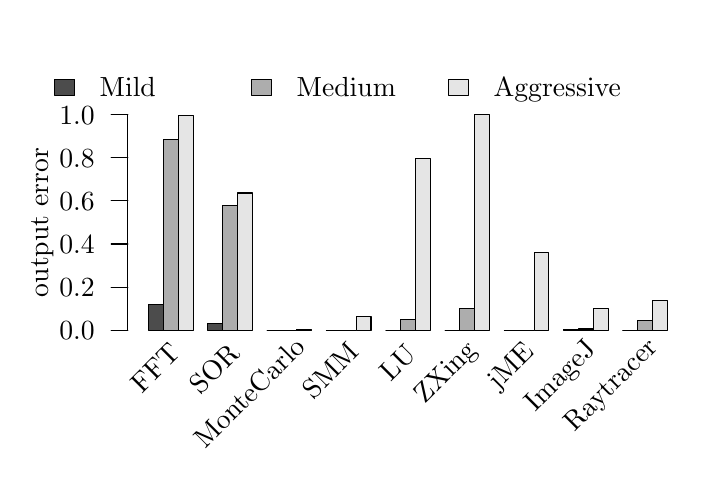
\begin{tikzpicture}[x=1pt,y=1pt]
\draw[color=white,opacity=0] (0,0) rectangle (238.49,151.77);
\begin{scope}
\path[clip] (  0.00,  0.00) rectangle (238.49,151.77);
\definecolor[named]{drawColor}{rgb}{0.18,0.00,0.42}
\definecolor[named]{fillColor}{rgb}{0.45,0.45,0.18}
\definecolor[named]{drawColor}{rgb}{0.00,0.00,0.00}
\definecolor[named]{fillColor}{rgb}{0.30,0.30,0.30}

\draw[color=drawColor,line cap=round,line join=round,fill=fillColor,] ( 43.50, 42.60) rectangle ( 48.86, 51.92);
\definecolor[named]{fillColor}{rgb}{0.68,0.68,0.68}

\draw[color=drawColor,line cap=round,line join=round,fill=fillColor,] ( 48.86, 42.60) rectangle ( 54.21,111.42);
\definecolor[named]{fillColor}{rgb}{0.90,0.90,0.90}

\draw[color=drawColor,line cap=round,line join=round,fill=fillColor,] ( 54.21, 42.60) rectangle ( 59.57,120.23);
\definecolor[named]{fillColor}{rgb}{0.30,0.30,0.30}

\draw[color=drawColor,line cap=round,line join=round,fill=fillColor,] ( 64.93, 42.60) rectangle ( 70.28, 45.09);
\definecolor[named]{fillColor}{rgb}{0.68,0.68,0.68}

\draw[color=drawColor,line cap=round,line join=round,fill=fillColor,] ( 70.28, 42.60) rectangle ( 75.64, 87.67);
\definecolor[named]{fillColor}{rgb}{0.90,0.90,0.90}

\draw[color=drawColor,line cap=round,line join=round,fill=fillColor,] ( 75.64, 42.60) rectangle ( 81.00, 92.21);
\definecolor[named]{fillColor}{rgb}{0.30,0.30,0.30}

\draw[color=drawColor,line cap=round,line join=round,fill=fillColor,] ( 86.35, 42.60) rectangle ( 91.71, 42.60);
\definecolor[named]{fillColor}{rgb}{0.68,0.68,0.68}

\draw[color=drawColor,line cap=round,line join=round,fill=fillColor,] ( 91.71, 42.60) rectangle ( 97.07, 42.61);
\definecolor[named]{fillColor}{rgb}{0.90,0.90,0.90}

\draw[color=drawColor,line cap=round,line join=round,fill=fillColor,] ( 97.07, 42.60) rectangle (102.43, 42.85);
\definecolor[named]{fillColor}{rgb}{0.30,0.30,0.30}

\draw[color=drawColor,line cap=round,line join=round,fill=fillColor,] (107.78, 42.60) rectangle (113.14, 42.60);
\definecolor[named]{fillColor}{rgb}{0.68,0.68,0.68}

\draw[color=drawColor,line cap=round,line join=round,fill=fillColor,] (113.14, 42.60) rectangle (118.50, 42.60);
\definecolor[named]{fillColor}{rgb}{0.90,0.90,0.90}

\draw[color=drawColor,line cap=round,line join=round,fill=fillColor,] (118.50, 42.60) rectangle (123.85, 47.53);
\definecolor[named]{fillColor}{rgb}{0.30,0.30,0.30}

\draw[color=drawColor,line cap=round,line join=round,fill=fillColor,] (129.21, 42.60) rectangle (134.57, 42.60);
\definecolor[named]{fillColor}{rgb}{0.68,0.68,0.68}

\draw[color=drawColor,line cap=round,line join=round,fill=fillColor,] (134.57, 42.60) rectangle (139.92, 46.64);
\definecolor[named]{fillColor}{rgb}{0.90,0.90,0.90}

\draw[color=drawColor,line cap=round,line join=round,fill=fillColor,] (139.92, 42.60) rectangle (145.28,104.67);
\definecolor[named]{fillColor}{rgb}{0.30,0.30,0.30}

\draw[color=drawColor,line cap=round,line join=round,fill=fillColor,] (150.64, 42.60) rectangle (155.99, 42.60);
\definecolor[named]{fillColor}{rgb}{0.68,0.68,0.68}

\draw[color=drawColor,line cap=round,line join=round,fill=fillColor,] (155.99, 42.60) rectangle (161.35, 50.40);
\definecolor[named]{fillColor}{rgb}{0.90,0.90,0.90}

\draw[color=drawColor,line cap=round,line join=round,fill=fillColor,] (161.35, 42.60) rectangle (166.71,120.57);
\definecolor[named]{fillColor}{rgb}{0.30,0.30,0.30}

\draw[color=drawColor,line cap=round,line join=round,fill=fillColor,] (172.07, 42.60) rectangle (177.42, 42.60);
\definecolor[named]{fillColor}{rgb}{0.68,0.68,0.68}

\draw[color=drawColor,line cap=round,line join=round,fill=fillColor,] (177.42, 42.60) rectangle (182.78, 42.60);
\definecolor[named]{fillColor}{rgb}{0.90,0.90,0.90}

\draw[color=drawColor,line cap=round,line join=round,fill=fillColor,] (182.78, 42.60) rectangle (188.14, 70.78);
\definecolor[named]{fillColor}{rgb}{0.30,0.30,0.30}

\draw[color=drawColor,line cap=round,line join=round,fill=fillColor,] (193.49, 42.60) rectangle (198.85, 42.85);
\definecolor[named]{fillColor}{rgb}{0.68,0.68,0.68}

\draw[color=drawColor,line cap=round,line join=round,fill=fillColor,] (198.85, 42.60) rectangle (204.21, 43.07);
\definecolor[named]{fillColor}{rgb}{0.90,0.90,0.90}

\draw[color=drawColor,line cap=round,line join=round,fill=fillColor,] (204.21, 42.60) rectangle (209.56, 50.54);
\definecolor[named]{fillColor}{rgb}{0.30,0.30,0.30}

\draw[color=drawColor,line cap=round,line join=round,fill=fillColor,] (214.92, 42.60) rectangle (220.28, 42.61);
\definecolor[named]{fillColor}{rgb}{0.68,0.68,0.68}

\draw[color=drawColor,line cap=round,line join=round,fill=fillColor,] (220.28, 42.60) rectangle (225.63, 46.15);
\definecolor[named]{fillColor}{rgb}{0.90,0.90,0.90}

\draw[color=drawColor,line cap=round,line join=round,fill=fillColor,] (225.63, 42.60) rectangle (230.99, 53.23);
\end{scope}
\begin{scope}
\path[clip] (  0.00,  0.00) rectangle (238.49,151.77);
\definecolor[named]{drawColor}{rgb}{0.18,0.00,0.42}
\definecolor[named]{fillColor}{rgb}{0.45,0.45,0.18}
\definecolor[named]{drawColor}{rgb}{0.00,0.00,0.00}

\draw[color=drawColor,line cap=round,line join=round,fill opacity=0.00,] ( 36.00, 42.60) -- ( 36.00,120.57);

\draw[color=drawColor,line cap=round,line join=round,fill opacity=0.00,] ( 36.00, 42.60) -- ( 30.00, 42.60);

\draw[color=drawColor,line cap=round,line join=round,fill opacity=0.00,] ( 36.00, 58.19) -- ( 30.00, 58.19);

\draw[color=drawColor,line cap=round,line join=round,fill opacity=0.00,] ( 36.00, 73.79) -- ( 30.00, 73.79);

\draw[color=drawColor,line cap=round,line join=round,fill opacity=0.00,] ( 36.00, 89.38) -- ( 30.00, 89.38);

\draw[color=drawColor,line cap=round,line join=round,fill opacity=0.00,] ( 36.00,104.97) -- ( 30.00,104.97);

\draw[color=drawColor,line cap=round,line join=round,fill opacity=0.00,] ( 36.00,120.57) -- ( 30.00,120.57);

\node[color=drawColor,anchor=base east,inner sep=0pt, outer sep=0pt, scale=  1.00] at ( 24.00, 39.16) {0.0%
};

\node[color=drawColor,anchor=base east,inner sep=0pt, outer sep=0pt, scale=  1.00] at ( 24.00, 54.75) {0.2%
};

\node[color=drawColor,anchor=base east,inner sep=0pt, outer sep=0pt, scale=  1.00] at ( 24.00, 70.34) {0.4%
};

\node[color=drawColor,anchor=base east,inner sep=0pt, outer sep=0pt, scale=  1.00] at ( 24.00, 85.94) {0.6%
};

\node[color=drawColor,anchor=base east,inner sep=0pt, outer sep=0pt, scale=  1.00] at ( 24.00,101.53) {0.8%
};

\node[color=drawColor,anchor=base east,inner sep=0pt, outer sep=0pt, scale=  1.00] at ( 24.00,117.12) {1.0%
};

\node[rotate= 90.00,color=drawColor,anchor=base,inner sep=0pt, outer sep=0pt, scale=  1.00] at (  7.20, 81.58) {output error%
};
\end{scope}
\begin{scope}
\path[clip] (  0.00,  0.00) rectangle (238.49,151.77);
\definecolor[named]{drawColor}{rgb}{0.18,0.00,0.42}
\definecolor[named]{fillColor}{rgb}{0.45,0.45,0.18}
\definecolor[named]{drawColor}{rgb}{0.00,0.00,0.00}
\definecolor[named]{fillColor}{rgb}{0.30,0.30,0.30}

\draw[color=drawColor,line cap=round,line join=round,fill=fillColor,] (  9.64,133.40) rectangle ( 16.84,127.40);
\definecolor[named]{fillColor}{rgb}{0.68,0.68,0.68}

\draw[color=drawColor,line cap=round,line join=round,fill=fillColor,] ( 80.81,133.40) rectangle ( 88.01,127.40);
\definecolor[named]{fillColor}{rgb}{0.90,0.90,0.90}

\draw[color=drawColor,line cap=round,line join=round,fill=fillColor,] (151.97,133.40) rectangle (159.17,127.40);

\node[color=drawColor,anchor=base west,inner sep=0pt, outer sep=0pt, scale=  1.00] at ( 25.84,126.95) {Mild%
};

\node[color=drawColor,anchor=base west,inner sep=0pt, outer sep=0pt, scale=  1.00] at ( 97.01,126.95) {Medium%
};

\node[color=drawColor,anchor=base west,inner sep=0pt, outer sep=0pt, scale=  1.00] at (168.17,126.95) {Aggressive%
};

\node[rotate= 45.00,color=drawColor,anchor=base east,inner sep=0pt, outer sep=0pt, scale=  1.00] at ( 55.40, 33.80) {FFT%
};

\node[rotate= 45.00,color=drawColor,anchor=base east,inner sep=0pt, outer sep=0pt, scale=  1.00] at ( 76.86, 33.83) {SOR%
};

\node[rotate= 45.00,color=drawColor,anchor=base east,inner sep=0pt, outer sep=0pt, scale=  1.00] at (100.48, 36.02) {MonteCarlo%
};

\node[rotate= 45.00,color=drawColor,anchor=base east,inner sep=0pt, outer sep=0pt, scale=  1.00] at (119.94, 34.06) {SMM%
};

\node[rotate= 45.00,color=drawColor,anchor=base east,inner sep=0pt, outer sep=0pt, scale=  1.00] at (140.65, 33.34) {LU%
};

\node[rotate= 45.00,color=drawColor,anchor=base east,inner sep=0pt, outer sep=0pt, scale=  1.00] at (162.33, 34.96) {ZXing%
};

\node[rotate= 45.00,color=drawColor,anchor=base east,inner sep=0pt, outer sep=0pt, scale=  1.00] at (183.19, 34.40) {jME%
};

\node[rotate= 45.00,color=drawColor,anchor=base east,inner sep=0pt, outer sep=0pt, scale=  1.00] at (205.50, 35.28) {ImageJ%
};

\node[rotate= 45.00,color=drawColor,anchor=base east,inner sep=0pt, outer sep=0pt, scale=  1.00] at (227.74, 36.09) {Raytracer%
};
\end{scope}
\end{tikzpicture}

\vspace{-4ex} % mysterious gap
\caption{Output error for three different levels of approximation varied
together. Each bar represents the mean error over 20 runs.}
\label{enerj:fig:sensitivity}
\end{figure}

Figure~\ref{enerj:fig:sensitivity} presents the sensitivity of each
annotated application to the full suite of approximations
explored. This quality-of-service reduction is the tradeoff for the
energy savings shown in Figure~\ref{enerj:fig:energy}.

While most applications show negligible error for the Mild level of
approximation, applications' sensitivity to error varies greatly for the Medium
and Aggressive configurations. Notably, MonteCarlo, SparseMatMult, ImageJ, and
Raytracer exhibit
very little output degradation under any configuration whereas FFT and SOR lose
significant output fidelity even under the Medium configuration.
This variation suggests that an approximate execution substrate for EnerJ
could benefit from tuning to the characteristics of each application,
either offline via profiling or online via continuous QoS measurement
as in Green \cite{green}.
However, even the
conservative Mild configuration offers significant energy savings.

Qualitatively, the approximated applications exhibit gradual degradation of
perceptible output quality. For instance, Raytracer always outputs an image
resembling its precise output, but the amount of random pixel ``noise''
increases with the aggressiveness of approximation. Under the Mild
configuration, it is difficult to distinguish the approximated image from the
precise one.

We also measured the relative impact of various approximation
strategies by running our benchmark suite with each optimization enabled in
isolation. DRAM errors have a nearly negligible impact on application output;
floating-point bit width reduction similarly results in at most 12\% QoS loss
in the Aggressive configuration. SRAM write errors are much more detrimental to
output quality than read upsets. Functional unit voltage reduction had the
greatest impact on correctness. We considered three possibilities for error
modes in
functional units: the output has a single bit flip; the last value computed is
returned; or a random value is returned. The former two models resulted in
significantly less QoS loss than the random-value model (25\% vs.~40\%).
However, we consider the random-value model to be the most realistic, so we use it for
the results shown in Figure~\ref{enerj:fig:sensitivity}.

\subsection{Annotation Effort}
\label{enerj:effort}
Table~\ref{enerj:table:applications} lists the number of qualifiers and
endorsements used in our annotations.
Only a fraction of the types in each program must be annotated: at most 34\% of
the possible annotation sites are used.
Note that most of the applications are short programs implementing a
single algorithm (the table shows the lines of code in
each program). Our largest application, ZXing, has about 26,000 lines
of code and only 4\% of its declarations are annotated.
These rates suggest that the principal data
amenable to approximation is concentrated in a small portion of the code,
even though approximate data typically dominates the program's dynamic behavior.

Endorsements are also rare, even though our system requires one for every
approximate condition value. The outlier is ZXing, which exhibits a higher
number of endorsements due to its frequency of approximate conditions. This is
because ZXing's control flow
frequently depends on whether a particular pixel is black.

Qualitatively, we found EnerJ's annotations easy to insert. The programmer
can typically select a small set of data to approximate and then, guided by type
checking errors, ascertain associated data that must also be marked as
approximate. The requirements that conditions and array indices be precise
helped quickly distinguish data that was likely to be sensitive to error. In
some cases, such as jMonkeyEngine and Raytracer, annotation was so
straightforward that it could have been largely automated: for certain methods,
every \ilcode{float} declaration was replaced indiscriminately with an
\ilcode{@Approx float} declaration.

Classes that closely represent data are perfect candidates for
\ilcode{@Approximable} annotations. For instance, ZXing contains
\ilcode{BitArray} and \ilcode{BitMatrix} classes that are thin wrappers over
binary data. It is useful to have approximate bit matrices in some settings (e.g.,
during image processing) but precise matrices in other settings (e.g., in
checksum calculation). Similarly, the jMonkeyEngine benchmark uses a
\ilcode{Vector3f} class for much of its computation, which we marked
as approximable.
In this setting, approximate vector declarations
(\ilcode{@Approx Vector3f v})
are syntactically identical to
approximate primitive-value declarations (\ilcode{@Approx int i}).

We found that the \ilcode{@Context} annotation helped us to approach program
annotation incrementally. A commonly-used class that is a target for
approximation can be marked with \ilcode{@Context} members instead of
\ilcode{@Approx} members. This way, all the clients of the class continue to
see precise members and no additional annotation on them is immediately
necessary. The programmer can then update the clients individually to use the
approximate version of the class rather than addressing the whole program at
once.

An opportunity for algorithmic approximation also arose in ZXing. The
\ilcode{BitArray} approximable class contains a method \ilcode{isRange} that
takes two indices and determines whether all the bits between the
two indices are set. We implemented an approximate version of the method that
checks only some of the bits in the range by skipping some loop iterations.
We believe that application domain experts would use algorithmic
approximation more frequently.

In one case, we found it convenient to introduce a slight change to increase the
fault tolerance of code dealing with approximate data. ZXing has a principally
floating-point phase that performs an image perspective transform. If the
transform tried to access a coordinate outside of the image bounds,
ZXing would catch the \ilcode{ArrayIndexOutOfBoundsException} and print a
message saying that the image transform failed. We modified the algorithm to
silently return a white pixel in this case. The result was that the image
transform became more resilient to transient faults in the transformation
coordinates. We marked these coordinates as
approximate and then endorsed them at the point they are used as array
indices.
In no case, however, does an application as we annotated it do
\emph{more} computation than the pristine version.


\section{Related Work}
\label{enerj:sec:rel}

Space constraints preclude a discussion of the vast body of compiler
or hybrid hardware/software work to improve energy efficiency.
Instead, we focus on work we are aware of that exploits approximate
computing to improve energy.

Many studies have shown that a variety of applications have a high
tolerance to transient faults \cite{dekruijf-selse09, li07, ersa,
  softcomputing, wong-selse06, qosprof}. However, certain parts of
programs are typically more fault-tolerant than others. Our work
exploits this property by allowing the programmer to distinguish
critical from non-critical computation.

Our work at the language level was influenced by previous work on
techniques for trading off correctness for power
savings. Flikker~\cite{flikker} proposes a programming model for
reducing the DRAM refresh rate on certain heap data via low-level
program annotations. Besides being limited to heap storage, Flikker does not
provide any safety guarantees. Relax~\cite{relax} is an architecture
that exposes timing faults to software as opposed to providing error
recovery automatically in hardware; its goal is to improve error
tolerance with lower power by exploiting portions of code that are
tolerant to error. While Relax focuses on error
recovery and hardware design simplicity, EnerJ emphasizes
energy-efficiency over error detectability and supports a wider range
of power-saving approximations. Moreover, Relax explores a
\emph{code-centric} approach, in which blocks of code are marked for
failure and recovery while EnerJ employs \emph{data-centric} type
annotations.

Work by Rinard et al.
proposes approximate code transformations in the compiler
\cite{perforationtr, qosprof, rinard-onward}.
Relatedly,
EnerJ's support for algorithmic approximation, the ability to write an
approximate implementation and a precise implementation of the same
functionality, bears some similarity to the Green programming
model~\cite{green}. However, Green primarily concerns itself with
online monitoring of application QoS; EnerJ's guarantees are entirely
static. Overall, EnerJ's type system makes approximation-based
approaches to energy savings general (it supports approximate
operations, storage, and algorithms) and safe (it provides static
isolation guarantees).

Using types to achieve fine-grained isolation of program
components is inspired by work on information flow types for secure
programming~\cite{infflow-survey,jif}. That body of work also influenced
the \emph{endorsement} construct for explicitly violating
non-interference.

Work by Perry et al. also focuses on static verification of fault tolerance
\cite{perry-pldi,perry-sas}. That work focuses on detection and
recovery rather than exposing transient faults.


% \section{Future Work}
% \label{enerj:sec:future}
%
% While the evaluation in this paper gives a rough picture of the potential
% energy savings offered by EnerJ and underlying approximate hardware, future
% evaluation of the EnerJ programming model should perform full-system simulation
% or experiment with real hardware.
%
% Extensions to EnerJ could explore the implications of approximation on standard
% libraries and system functions such as I/O. EnerJ reuses Java's standard class
% library in an entirely approximate way; there may be opportunity for energy
% savings in I/O, storage, and other platform functionality.
% \TODO{Aren't we using the JDK in an entirely \emph{precise} way?}
%
% As mentioned in Section~\ref{enerj:conditionals}, the present version of EnerJ
% simplifies control flow checking by requiring that all conditions on jumps be
% precise. This restriction is obviously conservative; more sophisticated
% implementations of the language could explore specialized control flow
% structures that permit approximate conditions.
%
% Our formalization of EnerJ does not model endorsement, which is
% designed to break the strict separation of approximate and precise
% program segments. A more complex formalization might provide weaker
% guarantees even in the presence of endorsement.
%
% EnerJ as presented provides an approximate/precise dichotomy with no bounds on
% \emph{how} approximate the values may be. While we have shown that even this
% simple model allows significant energy savings and reasonable safety
% guarantees, future work may explore a continuum from fully approximate data to
% fully precise data. More work could also guarantee approximation bounds: each
% variable could be guaranteed not to vary from its precise value by more than a
% certain bound as described in \cite{stanleymarbell}.
%
% EnerJ's framework for general approximation permits a wide variety of
% approximation strategies; here, we only explore a few of them. In particular,
% unsound compiler transformations as advocated in \cite{rinard-onward} may be
% well-suited to EnerJ programs.
%
% The simulation infrastructure used in the evaluation of EnerJ can inject
% arbitrary errors into storage and computation. As such, by permuting the
% location and magnitude of simulated faults, the infrastructure could be used to
% automatically discover the portions of an application that are amenable to
% approximation. This amounts to a ``quality-of-service profiler'' as proposed in
% \cite{qosprof} but discovers fault tolerance at a level more granular than
% loops.


\section{Conclusion}
\label{enerj:sec:conc}

Approximate computing is a very promising way of saving energy in
large classes of applications running on a wide range of systems, from
embedded systems to mobile phones to servers. We propose to use
a type system based on information-flow tracking ideas: variables and
objects can be declared as approximate or precise; approximate data can
be processed more cheaply and less reliably; and we can statically
prove that approximate data does not unexpectedly affect the precise
state of a program.
Our type system provides a general way of using approximation:
we can use approximate storage by mapping data to cheaper memory,
cache, and registers; we can use approximate operations by generating
code with cheaper, approximate instructions; and we can use method
overloading and class parameterization to enable algorithmic
approximation.

We implement our type system on top of Java and experiment with
several applications, from scientific computing to image processing to
games. Our results show that annotations are easy to insert:
only a fraction of declarations must be annotated and endorsements are
rare. Once a program is annotated for approximation, the runtime
system or architecture can choose several approximate execution
techniques. Our hardware-based model shows potential energy savings
between 7\% and 38\%.
